\documentclass{report}

%%%%%%%%%%%%%%%%%%%%%%%%%%%%%%%%%
% PACKAGE IMPORTS
%%%%%%%%%%%%%%%%%%%%%%%%%%%%%%%%%


\usepackage[tmargin=2cm,rmargin=1in,lmargin=1in,margin=0.85in,bmargin=2cm,footskip=.2in]{geometry}
\usepackage{amsmath,amsfonts,amsthm,amssymb,mathtools}
\usepackage[varbb]{newpxmath}
\usepackage{xfrac}
\usepackage[makeroom]{cancel}
\usepackage{mathtools}
\usepackage{bookmark}
\usepackage{enumitem}
\usepackage{hyperref,theoremref}
\hypersetup{
	pdftitle={Assignment},
	colorlinks=true, linkcolor=doc!90,
	bookmarksnumbered=true,
	bookmarksopen=true
}
\usepackage[most,many,breakable]{tcolorbox}
\usepackage{xcolor}
\usepackage{varwidth}
\usepackage{varwidth}
\usepackage{etoolbox}
%\usepackage{authblk}
\usepackage{nameref}
\usepackage{multicol,array}
\usepackage{tikz-cd}
\usepackage[ruled,vlined,linesnumbered]{algorithm2e}
\usepackage{comment} % enables the use of multi-line comments (\ifx \fi) 
\usepackage{import}
\usepackage{xifthen}
\usepackage{pdfpages}
\usepackage{transparent}

\newcommand\mycommfont[1]{\footnotesize\ttfamily\textcolor{blue}{#1}}
\SetCommentSty{mycommfont}
\newcommand{\incfig}[1]{%
    \def\svgwidth{\columnwidth}
    \import{./figures/}{#1.pdf_tex}
}

\usepackage{tikzsymbols}
\renewcommand\qedsymbol{$\Laughey$}


%\usepackage{import}
%\usepackage{xifthen}
%\usepackage{pdfpages}
%\usepackage{transparent}


%%%%%%%%%%%%%%%%%%%%%%%%%%%%%%
% SELF MADE COLORS
%%%%%%%%%%%%%%%%%%%%%%%%%%%%%%



\definecolor{myg}{RGB}{56, 140, 70}
\definecolor{myb}{RGB}{45, 111, 177}
\definecolor{myr}{RGB}{199, 68, 64}
\definecolor{mytheorembg}{HTML}{F2F2F9}
\definecolor{mytheoremfr}{HTML}{00007B}
\definecolor{mylenmabg}{HTML}{FFFAF8}
\definecolor{mylenmafr}{HTML}{983b0f}
\definecolor{mypropbg}{HTML}{f2fbfc}
\definecolor{mypropfr}{HTML}{191971}
\definecolor{myexamplebg}{HTML}{F2FBF8}
\definecolor{myexamplefr}{HTML}{88D6D1}
\definecolor{myexampleti}{HTML}{2A7F7F}
\definecolor{mydefinitbg}{HTML}{E5E5FF}
\definecolor{mydefinitfr}{HTML}{3F3FA3}
\definecolor{notesgreen}{RGB}{0,162,0}
\definecolor{myp}{RGB}{197, 92, 212}
\definecolor{mygr}{HTML}{2C3338}
\definecolor{myred}{RGB}{127,0,0}
\definecolor{myyellow}{RGB}{169,121,69}
\definecolor{myexercisebg}{HTML}{F2FBF8}
\definecolor{myexercisefg}{HTML}{88D6D1}


%%%%%%%%%%%%%%%%%%%%%%%%%%%%
% TCOLORBOX SETUPS
%%%%%%%%%%%%%%%%%%%%%%%%%%%%

\setlength{\parindent}{1cm}
%================================
% THEOREM BOX
%================================

\tcbuselibrary{theorems,skins,hooks}
\newtcbtheorem[number within=section]{Theorem}{Theorem}
{%
	enhanced,
	breakable,
	colback = mytheorembg,
	frame hidden,
	boxrule = 0sp,
	borderline west = {2pt}{0pt}{mytheoremfr},
	sharp corners,
	detach title,
	before upper = \tcbtitle\par\smallskip,
	coltitle = mytheoremfr,
	fonttitle = \bfseries\sffamily,
	description font = \mdseries,
	separator sign none,
	segmentation style={solid, mytheoremfr},
}
{th}

\tcbuselibrary{theorems,skins,hooks}
\newtcbtheorem[number within=chapter]{theorem}{Theorem}
{%
	enhanced,
	breakable,
	colback = mytheorembg,
	frame hidden,
	boxrule = 0sp,
	borderline west = {2pt}{0pt}{mytheoremfr},
	sharp corners,
	detach title,
	before upper = \tcbtitle\par\smallskip,
	coltitle = mytheoremfr,
	fonttitle = \bfseries\sffamily,
	description font = \mdseries,
	separator sign none,
	segmentation style={solid, mytheoremfr},
}
{th}


\tcbuselibrary{theorems,skins,hooks}
\newtcolorbox{Theoremcon}
{%
	enhanced
	,breakable
	,colback = mytheorembg
	,frame hidden
	,boxrule = 0sp
	,borderline west = {2pt}{0pt}{mytheoremfr}
	,sharp corners
	,description font = \mdseries
	,separator sign none
}

%================================
% Corollery
%================================
\tcbuselibrary{theorems,skins,hooks}
\newtcbtheorem[number within=section]{Corollary}{Corollary}
{%
	enhanced
	,breakable
	,colback = myp!10
	,frame hidden
	,boxrule = 0sp
	,borderline west = {2pt}{0pt}{myp!85!black}
	,sharp corners
	,detach title
	,before upper = \tcbtitle\par\smallskip
	,coltitle = myp!85!black
	,fonttitle = \bfseries\sffamily
	,description font = \mdseries
	,separator sign none
	,segmentation style={solid, myp!85!black}
}
{th}
\tcbuselibrary{theorems,skins,hooks}
\newtcbtheorem[number within=chapter]{corollary}{Corollary}
{%
	enhanced
	,breakable
	,colback = myp!10
	,frame hidden
	,boxrule = 0sp
	,borderline west = {2pt}{0pt}{myp!85!black}
	,sharp corners
	,detach title
	,before upper = \tcbtitle\par\smallskip
	,coltitle = myp!85!black
	,fonttitle = \bfseries\sffamily
	,description font = \mdseries
	,separator sign none
	,segmentation style={solid, myp!85!black}
}
{th}


%================================
% LENMA
%================================

\tcbuselibrary{theorems,skins,hooks}
\newtcbtheorem[number within=section]{Lenma}{Lenma}
{%
	enhanced,
	breakable,
	colback = mylenmabg,
	frame hidden,
	boxrule = 0sp,
	borderline west = {2pt}{0pt}{mylenmafr},
	sharp corners,
	detach title,
	before upper = \tcbtitle\par\smallskip,
	coltitle = mylenmafr,
	fonttitle = \bfseries\sffamily,
	description font = \mdseries,
	separator sign none,
	segmentation style={solid, mylenmafr},
}
{th}

\tcbuselibrary{theorems,skins,hooks}
\newtcbtheorem[number within=chapter]{lenma}{Lenma}
{%
	enhanced,
	breakable,
	colback = mylenmabg,
	frame hidden,
	boxrule = 0sp,
	borderline west = {2pt}{0pt}{mylenmafr},
	sharp corners,
	detach title,
	before upper = \tcbtitle\par\smallskip,
	coltitle = mylenmafr,
	fonttitle = \bfseries\sffamily,
	description font = \mdseries,
	separator sign none,
	segmentation style={solid, mylenmafr},
}
{th}


%================================
% PROPOSITION
%================================

\tcbuselibrary{theorems,skins,hooks}
\newtcbtheorem[number within=section]{Prop}{Proposition}
{%
	enhanced,
	breakable,
	colback = mypropbg,
	frame hidden,
	boxrule = 0sp,
	borderline west = {2pt}{0pt}{mypropfr},
	sharp corners,
	detach title,
	before upper = \tcbtitle\par\smallskip,
	coltitle = mypropfr,
	fonttitle = \bfseries\sffamily,
	description font = \mdseries,
	separator sign none,
	segmentation style={solid, mypropfr},
}
{th}

\tcbuselibrary{theorems,skins,hooks}
\newtcbtheorem[number within=chapter]{prop}{Proposition}
{%
	enhanced,
	breakable,
	colback = mypropbg,
	frame hidden,
	boxrule = 0sp,
	borderline west = {2pt}{0pt}{mypropfr},
	sharp corners,
	detach title,
	before upper = \tcbtitle\par\smallskip,
	coltitle = mypropfr,
	fonttitle = \bfseries\sffamily,
	description font = \mdseries,
	separator sign none,
	segmentation style={solid, mypropfr},
}
{th}


%================================
% CLAIM
%================================

\tcbuselibrary{theorems,skins,hooks}
\newtcbtheorem[number within=section]{claim}{Claim}
{%
	enhanced
	,breakable
	,colback = myg!10
	,frame hidden
	,boxrule = 0sp
	,borderline west = {2pt}{0pt}{myg}
	,sharp corners
	,detach title
	,before upper = \tcbtitle\par\smallskip
	,coltitle = myg!85!black
	,fonttitle = \bfseries\sffamily
	,description font = \mdseries
	,separator sign none
	,segmentation style={solid, myg!85!black}
}
{th}



%================================
% Exercise
%================================

\tcbuselibrary{theorems,skins,hooks}
\newtcbtheorem[number within=section]{Exercise}{Exercise}
{%
	enhanced,
	breakable,
	colback = myexercisebg,
	frame hidden,
	boxrule = 0sp,
	borderline west = {2pt}{0pt}{myexercisefg},
	sharp corners,
	detach title,
	before upper = \tcbtitle\par\smallskip,
	coltitle = myexercisefg,
	fonttitle = \bfseries\sffamily,
	description font = \mdseries,
	separator sign none,
	segmentation style={solid, myexercisefg},
}
{th}

\tcbuselibrary{theorems,skins,hooks}
\newtcbtheorem[number within=chapter]{exercise}{Exercise}
{%
	enhanced,
	breakable,
	colback = myexercisebg,
	frame hidden,
	boxrule = 0sp,
	borderline west = {2pt}{0pt}{myexercisefg},
	sharp corners,
	detach title,
	before upper = \tcbtitle\par\smallskip,
	coltitle = myexercisefg,
	fonttitle = \bfseries\sffamily,
	description font = \mdseries,
	separator sign none,
	segmentation style={solid, myexercisefg},
}
{th}

%================================
% EXAMPLE BOX
%================================

\newtcbtheorem[number within=section]{Example}{Example}
{%
	colback = myexamplebg
	,breakable
	,colframe = myexamplefr
	,coltitle = myexampleti
	,boxrule = 1pt
	,sharp corners
	,detach title
	,before upper=\tcbtitle\par\smallskip
	,fonttitle = \bfseries
	,description font = \mdseries
	,separator sign none
	,description delimiters parenthesis
}
{ex}

\newtcbtheorem[number within=chapter]{example}{Example}
{%
	colback = myexamplebg
	,breakable
	,colframe = myexamplefr
	,coltitle = myexampleti
	,boxrule = 1pt
	,sharp corners
	,detach title
	,before upper=\tcbtitle\par\smallskip
	,fonttitle = \bfseries
	,description font = \mdseries
	,separator sign none
	,description delimiters parenthesis
}
{ex}

%================================
% DEFINITION BOX
%================================

\newtcbtheorem[number within=section]{Definition}{Definition}{enhanced,
	before skip=2mm,after skip=2mm, colback=red!5,colframe=red!80!black,boxrule=0.5mm,
	attach boxed title to top left={xshift=1cm,yshift*=1mm-\tcboxedtitleheight}, varwidth boxed title*=-3cm,
	boxed title style={frame code={
					\path[fill=tcbcolback]
					([yshift=-1mm,xshift=-1mm]frame.north west)
					arc[start angle=0,end angle=180,radius=1mm]
					([yshift=-1mm,xshift=1mm]frame.north east)
					arc[start angle=180,end angle=0,radius=1mm];
					\path[left color=tcbcolback!60!black,right color=tcbcolback!60!black,
						middle color=tcbcolback!80!black]
					([xshift=-2mm]frame.north west) -- ([xshift=2mm]frame.north east)
					[rounded corners=1mm]-- ([xshift=1mm,yshift=-1mm]frame.north east)
					-- (frame.south east) -- (frame.south west)
					-- ([xshift=-1mm,yshift=-1mm]frame.north west)
					[sharp corners]-- cycle;
				},interior engine=empty,
		},
	fonttitle=\bfseries,
	title={#2},#1}{def}
\newtcbtheorem[number within=chapter]{definition}{Definition}{enhanced,
	before skip=2mm,after skip=2mm, colback=red!5,colframe=red!80!black,boxrule=0.5mm,
	attach boxed title to top left={xshift=1cm,yshift*=1mm-\tcboxedtitleheight}, varwidth boxed title*=-3cm,
	boxed title style={frame code={
					\path[fill=tcbcolback]
					([yshift=-1mm,xshift=-1mm]frame.north west)
					arc[start angle=0,end angle=180,radius=1mm]
					([yshift=-1mm,xshift=1mm]frame.north east)
					arc[start angle=180,end angle=0,radius=1mm];
					\path[left color=tcbcolback!60!black,right color=tcbcolback!60!black,
						middle color=tcbcolback!80!black]
					([xshift=-2mm]frame.north west) -- ([xshift=2mm]frame.north east)
					[rounded corners=1mm]-- ([xshift=1mm,yshift=-1mm]frame.north east)
					-- (frame.south east) -- (frame.south west)
					-- ([xshift=-1mm,yshift=-1mm]frame.north west)
					[sharp corners]-- cycle;
				},interior engine=empty,
		},
	fonttitle=\bfseries,
	title={#2},#1}{def}



%================================
% Solution BOX
%================================

\makeatletter
\newtcbtheorem{question}{Question}{enhanced,
	breakable,
	colback=white,
	colframe=myb!80!black,
	attach boxed title to top left={yshift*=-\tcboxedtitleheight},
	fonttitle=\bfseries,
	title={#2},
	boxed title size=title,
	boxed title style={%
			sharp corners,
			rounded corners=northwest,
			colback=tcbcolframe,
			boxrule=0pt,
		},
	underlay boxed title={%
			\path[fill=tcbcolframe] (title.south west)--(title.south east)
			to[out=0, in=180] ([xshift=5mm]title.east)--
			(title.center-|frame.east)
			[rounded corners=\kvtcb@arc] |-
			(frame.north) -| cycle;
		},
	#1
}{def}
\makeatother

%================================
% SOLUTION BOX
%================================

\makeatletter
\newtcolorbox{solution}{enhanced,
	breakable,
	colback=white,
	colframe=myg!80!black,
	attach boxed title to top left={yshift*=-\tcboxedtitleheight},
	title=Solution,
	boxed title size=title,
	boxed title style={%
			sharp corners,
			rounded corners=northwest,
			colback=tcbcolframe,
			boxrule=0pt,
		},
	underlay boxed title={%
			\path[fill=tcbcolframe] (title.south west)--(title.south east)
			to[out=0, in=180] ([xshift=5mm]title.east)--
			(title.center-|frame.east)
			[rounded corners=\kvtcb@arc] |-
			(frame.north) -| cycle;
		},
}
\makeatother

%================================
% Question BOX
%================================

\makeatletter
\newtcbtheorem{qstion}{Question}{enhanced,
	breakable,
	colback=white,
	colframe=mygr,
	attach boxed title to top left={yshift*=-\tcboxedtitleheight},
	fonttitle=\bfseries,
	title={#2},
	boxed title size=title,
	boxed title style={%
			sharp corners,
			rounded corners=northwest,
			colback=tcbcolframe,
			boxrule=0pt,
		},
	underlay boxed title={%
			\path[fill=tcbcolframe] (title.south west)--(title.south east)
			to[out=0, in=180] ([xshift=5mm]title.east)--
			(title.center-|frame.east)
			[rounded corners=\kvtcb@arc] |-
			(frame.north) -| cycle;
		},
	#1
}{def}
\makeatother

\newtcbtheorem[number within=chapter]{wconc}{Wrong Concept}{
	breakable,
	enhanced,
	colback=white,
	colframe=myr,
	arc=0pt,
	outer arc=0pt,
	fonttitle=\bfseries\sffamily\large,
	colbacktitle=myr,
	attach boxed title to top left={},
	boxed title style={
			enhanced,
			skin=enhancedfirst jigsaw,
			arc=3pt,
			bottom=0pt,
			interior style={fill=myr}
		},
	#1
}{def}



%================================
% NOTE BOX
%================================

\usetikzlibrary{arrows,calc,shadows.blur}
\tcbuselibrary{skins}
\newtcolorbox{note}[1][]{%
	enhanced jigsaw,
	colback=gray!20!white,%
	colframe=gray!80!black,
	size=small,
	boxrule=1pt,
	title=\textbf{Note:},
	halign title=flush center,
	coltitle=black,
	breakable,
	drop shadow=black!50!white,
	attach boxed title to top left={xshift=1cm,yshift=-\tcboxedtitleheight/2,yshifttext=-\tcboxedtitleheight/2},
	minipage boxed title=1.5cm,
	boxed title style={%
			colback=white,
			size=fbox,
			boxrule=1pt,
			boxsep=2pt,
			underlay={%
					\coordinate (dotA) at ($(interior.west) + (-0.5pt,0)$);
					\coordinate (dotB) at ($(interior.east) + (0.5pt,0)$);
					\begin{scope}
						\clip (interior.north west) rectangle ([xshift=3ex]interior.east);
						\filldraw [white, blur shadow={shadow opacity=60, shadow yshift=-.75ex}, rounded corners=2pt] (interior.north west) rectangle (interior.south east);
					\end{scope}
					\begin{scope}[gray!80!black]
						\fill (dotA) circle (2pt);
						\fill (dotB) circle (2pt);
					\end{scope}
				},
		},
	#1,
}

%%%%%%%%%%%%%%%%%%%%%%%%%%%%%%
% SELF MADE COMMANDS
%%%%%%%%%%%%%%%%%%%%%%%%%%%%%%


\newcommand{\thm}[2]{\begin{Theorem}{#1}{}#2\end{Theorem}}
\newcommand{\cor}[2]{\begin{Corollary}{#1}{}#2\end{Corollary}}
\newcommand{\mlenma}[2]{\begin{Lenma}{#1}{}#2\end{Lenma}}
\newcommand{\mprop}[2]{\begin{Prop}{#1}{}#2\end{Prop}}
\newcommand{\clm}[3]{\begin{claim}{#1}{#2}#3\end{claim}}
\newcommand{\wc}[2]{\begin{wconc}{#1}{}\setlength{\parindent}{1cm}#2\end{wconc}}
\newcommand{\thmcon}[1]{\begin{Theoremcon}{#1}\end{Theoremcon}}
\newcommand{\ex}[2]{\begin{Example}{#1}{}#2\end{Example}}
\newcommand{\dfn}[2]{\begin{Definition}[colbacktitle=red!75!black]{#1}{}#2\end{Definition}}
\newcommand{\dfnc}[2]{\begin{definition}[colbacktitle=red!75!black]{#1}{}#2\end{definition}}
\newcommand{\qs}[2]{\begin{question}{#1}{}#2\end{question}}
\newcommand{\pf}[2]{\begin{myproof}[#1]#2\end{myproof}}
\newcommand{\nt}[1]{\begin{note}#1\end{note}}

\newcommand*\circled[1]{\tikz[baseline=(char.base)]{
		\node[shape=circle,draw,inner sep=1pt] (char) {#1};}}
\newcommand\getcurrentref[1]{%
	\ifnumequal{\value{#1}}{0}
	{??}
	{\the\value{#1}}%
}
\newcommand{\getCurrentSectionNumber}{\getcurrentref{section}}
\newenvironment{myproof}[1][\proofname]{%
	\proof[\bfseries #1: ]%
}{\endproof}

\newcommand{\mclm}[2]{\begin{myclaim}[#1]#2\end{myclaim}}
\newenvironment{myclaim}[1][\claimname]{\proof[\bfseries #1: ]}{}

\newcounter{mylabelcounter}

\makeatletter
\newcommand{\setword}[2]{%
	\phantomsection
	#1\def\@currentlabel{\unexpanded{#1}}\label{#2}%
}
\makeatother




\tikzset{
	symbol/.style={
			draw=none,
			every to/.append style={
					edge node={node [sloped, allow upside down, auto=false]{$#1$}}}
		}
}


% deliminators
\DeclarePairedDelimiter{\abs}{\lvert}{\rvert}
\DeclarePairedDelimiter{\norm}{\lVert}{\rVert}

\DeclarePairedDelimiter{\ceil}{\lceil}{\rceil}
\DeclarePairedDelimiter{\floor}{\lfloor}{\rfloor}
\DeclarePairedDelimiter{\round}{\lfloor}{\rceil}

\newsavebox\diffdbox
\newcommand{\slantedromand}{{\mathpalette\makesl{d}}}
\newcommand{\makesl}[2]{%
\begingroup
\sbox{\diffdbox}{$\mathsurround=0pt#1\mathrm{#2}$}%
\pdfsave
\pdfsetmatrix{1 0 0.2 1}%
\rlap{\usebox{\diffdbox}}%
\pdfrestore
\hskip\wd\diffdbox
\endgroup
}
\newcommand{\dd}[1][]{\ensuremath{\mathop{}\!\ifstrempty{#1}{%
\slantedromand\@ifnextchar^{\hspace{0.2ex}}{\hspace{0.1ex}}}%
{\slantedromand\hspace{0.2ex}^{#1}}}}
\ProvideDocumentCommand\dv{o m g}{%
  \ensuremath{%
    \IfValueTF{#3}{%
      \IfNoValueTF{#1}{%
        \frac{\dd #2}{\dd #3}%
      }{%
        \frac{\dd^{#1} #2}{\dd #3^{#1}}%
      }%
    }{%
      \IfNoValueTF{#1}{%
        \frac{\dd}{\dd #2}%
      }{%
        \frac{\dd^{#1}}{\dd #2^{#1}}%
      }%
    }%
  }%
}
\providecommand*{\pdv}[3][]{\frac{\partial^{#1}#2}{\partial#3^{#1}}}
%  - others
\DeclareMathOperator{\Lap}{\mathcal{L}}
\DeclareMathOperator{\Var}{Var} % varience
\DeclareMathOperator{\Cov}{Cov} % covarience
\DeclareMathOperator{\E}{E} % expected

% Since the amsthm package isn't loaded

% I prefer the slanted \leq
\let\oldleq\leq % save them in case they're every wanted
\let\oldgeq\geq
\renewcommand{\leq}{\leqslant}
\renewcommand{\geq}{\geqslant}

% % redefine matrix env to allow for alignment, use r as default
% \renewcommand*\env@matrix[1][r]{\hskip -\arraycolsep
%     \let\@ifnextchar\new@ifnextchar
%     \array{*\c@MaxMatrixCols #1}}


%\usepackage{framed}
%\usepackage{titletoc}
%\usepackage{etoolbox}
%\usepackage{lmodern}


%\patchcmd{\tableofcontents}{\contentsname}{\sffamily\contentsname}{}{}

%\renewenvironment{leftbar}
%{\def\FrameCommand{\hspace{6em}%
%		{\color{myyellow}\vrule width 2pt depth 6pt}\hspace{1em}}%
%	\MakeFramed{\parshape 1 0cm \dimexpr\textwidth-6em\relax\FrameRestore}\vskip2pt%
%}
%{\endMakeFramed}

%\titlecontents{chapter}
%[0em]{\vspace*{2\baselineskip}}
%{\parbox{4.5em}{%
%		\hfill\Huge\sffamily\bfseries\color{myred}\thecontentspage}%
%	\vspace*{-2.3\baselineskip}\leftbar\textsc{\small\chaptername~\thecontentslabel}\\\sffamily}
%{}{\endleftbar}
%\titlecontents{section}
%[8.4em]
%{\sffamily\contentslabel{3em}}{}{}
%{\hspace{0.5em}\nobreak\itshape\color{myred}\contentspage}
%\titlecontents{subsection}
%[8.4em]
%{\sffamily\contentslabel{3em}}{}{}  
%{\hspace{0.5em}\nobreak\itshape\color{myred}\contentspage}



%%%%%%%%%%%%%%%%%%%%%%%%%%%%%%%%%%%%%%%%%%%
% TABLE OF CONTENTS
%%%%%%%%%%%%%%%%%%%%%%%%%%%%%%%%%%%%%%%%%%%

\usepackage{tikz}
\definecolor{doc}{RGB}{0,60,110}
\usepackage{titletoc}
\contentsmargin{0cm}
\titlecontents{chapter}[3.7pc]
{\addvspace{30pt}%
	\begin{tikzpicture}[remember picture, overlay]%
		\draw[fill=doc!60,draw=doc!60] (-7,-.1) rectangle (-0.9,.5);%
		\pgftext[left,x=-3.5cm,y=0.2cm]{\color{white}\Large\sc\bfseries Chapter\ \thecontentslabel};%
	\end{tikzpicture}\color{doc!60}\large\sc\bfseries}%
{}
{}
{\;\titlerule\;\large\sc\bfseries Page \thecontentspage
	\begin{tikzpicture}[remember picture, overlay]
		\draw[fill=doc!60,draw=doc!60] (2pt,0) rectangle (4,0.1pt);
	\end{tikzpicture}}%
\titlecontents{section}[3.7pc]
{\addvspace{2pt}}
{\contentslabel[\thecontentslabel]{2pc}}
{}
{\hfill\small \thecontentspage}
[]
\titlecontents*{subsection}[3.7pc]
{\addvspace{-1pt}\small}
{}
{}
{\ --- \small\thecontentspage}
[ \textbullet\ ][]

\makeatletter
\renewcommand{\tableofcontents}{%
	\chapter*{%
	  \vspace*{-20\p@}%
	  \begin{tikzpicture}[remember picture, overlay]%
		  \pgftext[right,x=15cm,y=0.2cm]{\color{doc!60}\Huge\sc\bfseries \contentsname};%
		  \draw[fill=doc!60,draw=doc!60] (13,-.75) rectangle (20,1);%
		  \clip (13,-.75) rectangle (20,1);
		  \pgftext[right,x=15cm,y=0.2cm]{\color{white}\Huge\sc\bfseries \contentsname};%
	  \end{tikzpicture}}%
	\@starttoc{toc}}
\makeatother


% My commands %
\newcommand{\innerproduct}[2]{\langle #1, #2 \rangle}
\newcommand{\generators}[1]{\langle #1 \rangle}

%From M275 "Topology" at SJSU
\newcommand{\id}{\mathrm{id}}
\newcommand{\taking}[1]{\xrightarrow{#1}}
\newcommand{\inv}{^{-1}}

%From M170 "Introduction to Graph Theory" at SJSU
\DeclareMathOperator{\diam}{diam}
\DeclareMathOperator{\ord}{ord}
\newcommand{\defeq}{\overset{\mathrm{def}}{=}}

%From the USAMO .tex files
\newcommand{\ts}{\textsuperscript}
\newcommand{\dg}{^\circ}
\newcommand{\ii}{\item}

% % From Math 55 and Math 145 at Harvard
% \newenvironment{subproof}[1][Proof]{%
% \begin{proof}[#1] \renewcommand{\qedsymbol}{$\blacksquare$}}%
% {\end{proof}}

\newcommand{\liff}{\leftrightarrow}
\newcommand{\lthen}{\rightarrow}
\newcommand{\opname}{\operatorname}
\newcommand{\surjto}{\twoheadrightarrow}
\newcommand{\injto}{\hookrightarrow}
\newcommand{\On}{\mathrm{On}} % ordinals
\DeclareMathOperator{\img}{im} % Image
\DeclareMathOperator{\Img}{Im} % Image
\DeclareMathOperator{\coker}{coker} % Cokernel
\DeclareMathOperator{\Coker}{Coker} % Cokernel
\DeclareMathOperator{\Ker}{Ker} % Kernel
\DeclareMathOperator{\rank}{rank}
\DeclareMathOperator{\Spec}{Spec} % spectrum
\DeclareMathOperator{\Tr}{Tr} % trace
\DeclareMathOperator{\pr}{pr} % projection
\DeclareMathOperator{\ext}{ext} % extension
\DeclareMathOperator{\pred}{pred} % predecessor
\DeclareMathOperator{\dom}{dom} % domain
\DeclareMathOperator{\ran}{ran} % range
\DeclareMathOperator{\Hom}{Hom} % homomorphism
\DeclareMathOperator{\Mor}{Mor} % morphisms
\DeclareMathOperator{\End}{End} % endomorphism

\newcommand{\eps}{\epsilon}
\newcommand{\veps}{\varepsilon}
\newcommand{\ol}{\overline}
\newcommand{\ul}{\underline}
\newcommand{\wt}{\widetilde}
\newcommand{\wh}{\widehat}
\newcommand{\vocab}[1]{\textbf{\color{blue} #1}}
\providecommand{\half}{\frac{1}{2}}
\newcommand{\dang}{\measuredangle} %% Directed angle
\newcommand{\ray}[1]{\overrightarrow{#1}}
\newcommand{\seg}[1]{\overline{#1}}
\newcommand{\arc}[1]{\wideparen{#1}}
\DeclareMathOperator{\cis}{cis}
\DeclareMathOperator*{\lcm}{lcm}
\DeclareMathOperator*{\argmin}{arg min}
\DeclareMathOperator*{\argmax}{arg max}
\newcommand{\cycsum}{\sum_{\mathrm{cyc}}}
\newcommand{\symsum}{\sum_{\mathrm{sym}}}
\newcommand{\cycprod}{\prod_{\mathrm{cyc}}}
\newcommand{\symprod}{\prod_{\mathrm{sym}}}
\newcommand{\Qed}{\begin{flushright}\qed\end{flushright}}
\newcommand{\parinn}{\setlength{\parindent}{1cm}}
\newcommand{\parinf}{\setlength{\parindent}{0cm}}
% \newcommand{\norm}{\|\cdot\|}
\newcommand{\inorm}{\norm_{\infty}}
\newcommand{\opensets}{\{V_{\alpha}\}_{\alpha\in I}}
\newcommand{\oset}{V_{\alpha}}
\newcommand{\opset}[1]{V_{\alpha_{#1}}}
\newcommand{\lub}{\text{lub}}
\newcommand{\del}[2]{\frac{\partial #1}{\partial #2}}
\newcommand{\Del}[3]{\frac{\partial^{#1} #2}{\partial^{#1} #3}}
\newcommand{\deld}[2]{\dfrac{\partial #1}{\partial #2}}
\newcommand{\Deld}[3]{\dfrac{\partial^{#1} #2}{\partial^{#1} #3}}
\newcommand{\lm}{\lambda}
\newcommand{\uin}{\mathbin{\rotatebox[origin=c]{90}{$\in$}}}
\newcommand{\usubset}{\mathbin{\rotatebox[origin=c]{90}{$\subset$}}}
\newcommand{\lt}{\left}
\newcommand{\rt}{\right}
\newcommand{\bs}[1]{\boldsymbol{#1}}
\newcommand{\exs}{\exists}
\newcommand{\st}{\strut}
\newcommand{\dps}[1]{\displaystyle{#1}}

\newcommand{\sol}{\setlength{\parindent}{0cm}\textbf{\textit{Solution:}}\setlength{\parindent}{1cm} }
\newcommand{\solve}[1]{\setlength{\parindent}{0cm}\textbf{\textit{Solution: }}\setlength{\parindent}{1cm}#1 \Qed}

% Things Lie
\newcommand{\kb}{\mathfrak b}
\newcommand{\kg}{\mathfrak g}
\newcommand{\kh}{\mathfrak h}
\newcommand{\kn}{\mathfrak n}
\newcommand{\ku}{\mathfrak u}
\newcommand{\kz}{\mathfrak z}
\DeclareMathOperator{\Ext}{Ext} % Ext functor
\DeclareMathOperator{\Tor}{Tor} % Tor functor
\newcommand{\gl}{\opname{\mathfrak{gl}}} % frak gl group
\renewcommand{\sl}{\opname{\mathfrak{sl}}} % frak sl group chktex 6

% More script letters etc.
\newcommand{\SA}{\mathcal A}
\newcommand{\SB}{\mathcal B}
\newcommand{\SC}{\mathcal C}
\newcommand{\SF}{\mathcal F}
\newcommand{\SG}{\mathcal G}
\newcommand{\SH}{\mathcal H}
\newcommand{\OO}{\mathcal O}

\newcommand{\SCA}{\mathscr A}
\newcommand{\SCB}{\mathscr B}
\newcommand{\SCC}{\mathscr C}
\newcommand{\SCD}{\mathscr D}
\newcommand{\SCE}{\mathscr E}
\newcommand{\SCF}{\mathscr F}
\newcommand{\SCG}{\mathscr G}
\newcommand{\SCH}{\mathscr H}

% Mathfrak primes
\newcommand{\km}{\mathfrak m}
\newcommand{\kp}{\mathfrak p}
\newcommand{\kq}{\mathfrak q}

% number sets
\newcommand{\RR}[1][]{\ensuremath{\ifstrempty{#1}{\mathbb{R}}{\mathbb{R}^{#1}}}}
\newcommand{\NN}[1][]{\ensuremath{\ifstrempty{#1}{\mathbb{N}}{\mathbb{N}^{#1}}}}
\newcommand{\ZZ}[1][]{\ensuremath{\ifstrempty{#1}{\mathbb{Z}}{\mathbb{Z}^{#1}}}}
\newcommand{\QQ}[1][]{\ensuremath{\ifstrempty{#1}{\mathbb{Q}}{\mathbb{Q}^{#1}}}}
\newcommand{\CC}[1][]{\ensuremath{\ifstrempty{#1}{\mathbb{C}}{\mathbb{C}^{#1}}}}
\newcommand{\PP}[1][]{\ensuremath{\ifstrempty{#1}{\mathbb{P}}{\mathbb{P}^{#1}}}}
\newcommand{\HH}[1][]{\ensuremath{\ifstrempty{#1}{\mathbb{H}}{\mathbb{H}^{#1}}}}
\newcommand{\FF}[1][]{\ensuremath{\ifstrempty{#1}{\mathbb{F}}{\mathbb{F}^{#1}}}}
% expected value
\newcommand{\EE}{\ensuremath{\mathbb{E}}}
\newcommand{\charin}{\text{ char }}
\DeclareMathOperator{\sign}{sign}
\DeclareMathOperator{\Aut}{Aut}
\DeclareMathOperator{\Inn}{Inn}
\DeclareMathOperator{\Syl}{Syl}
\DeclareMathOperator{\Gal}{Gal}
\DeclareMathOperator{\GL}{GL} % General linear group
\DeclareMathOperator{\SL}{SL} % Special linear group

%---------------------------------------
% BlackBoard Math Fonts :-
%---------------------------------------

%Captital Letters
\newcommand{\bbA}{\mathbb{A}}	\newcommand{\bbB}{\mathbb{B}}
\newcommand{\bbC}{\mathbb{C}}	\newcommand{\bbD}{\mathbb{D}}
\newcommand{\bbE}{\mathbb{E}}	\newcommand{\bbF}{\mathbb{F}}
\newcommand{\bbG}{\mathbb{G}}	\newcommand{\bbH}{\mathbb{H}}
\newcommand{\bbI}{\mathbb{I}}	\newcommand{\bbJ}{\mathbb{J}}
\newcommand{\bbK}{\mathbb{K}}	\newcommand{\bbL}{\mathbb{L}}
\newcommand{\bbM}{\mathbb{M}}	\newcommand{\bbN}{\mathbb{N}}
\newcommand{\bbO}{\mathbb{O}}	\newcommand{\bbP}{\mathbb{P}}
\newcommand{\bbQ}{\mathbb{Q}}	\newcommand{\bbR}{\mathbb{R}}
\newcommand{\bbS}{\mathbb{S}}	\newcommand{\bbT}{\mathbb{T}}
\newcommand{\bbU}{\mathbb{U}}	\newcommand{\bbV}{\mathbb{V}}
\newcommand{\bbW}{\mathbb{W}}	\newcommand{\bbX}{\mathbb{X}}
\newcommand{\bbY}{\mathbb{Y}}	\newcommand{\bbZ}{\mathbb{Z}}

%---------------------------------------
% MathCal Fonts :-
%---------------------------------------

%Captital Letters
\newcommand{\mcA}{\mathcal{A}}	\newcommand{\mcB}{\mathcal{B}}
\newcommand{\mcC}{\mathcal{C}}	\newcommand{\mcD}{\mathcal{D}}
\newcommand{\mcE}{\mathcal{E}}	\newcommand{\mcF}{\mathcal{F}}
\newcommand{\mcG}{\mathcal{G}}	\newcommand{\mcH}{\mathcal{H}}
\newcommand{\mcI}{\mathcal{I}}	\newcommand{\mcJ}{\mathcal{J}}
\newcommand{\mcK}{\mathcal{K}}	\newcommand{\mcL}{\mathcal{L}}
\newcommand{\mcM}{\mathcal{M}}	\newcommand{\mcN}{\mathcal{N}}
\newcommand{\mcO}{\mathcal{O}}	\newcommand{\mcP}{\mathcal{P}}
\newcommand{\mcQ}{\mathcal{Q}}	\newcommand{\mcR}{\mathcal{R}}
\newcommand{\mcS}{\mathcal{S}}	\newcommand{\mcT}{\mathcal{T}}
\newcommand{\mcU}{\mathcal{U}}	\newcommand{\mcV}{\mathcal{V}}
\newcommand{\mcW}{\mathcal{W}}	\newcommand{\mcX}{\mathcal{X}}
\newcommand{\mcY}{\mathcal{Y}}	\newcommand{\mcZ}{\mathcal{Z}}


%---------------------------------------
% Bold Math Fonts :-
%---------------------------------------

%Captital Letters
\newcommand{\bmA}{\boldsymbol{A}}	\newcommand{\bmB}{\boldsymbol{B}}
\newcommand{\bmC}{\boldsymbol{C}}	\newcommand{\bmD}{\boldsymbol{D}}
\newcommand{\bmE}{\boldsymbol{E}}	\newcommand{\bmF}{\boldsymbol{F}}
\newcommand{\bmG}{\boldsymbol{G}}	\newcommand{\bmH}{\boldsymbol{H}}
\newcommand{\bmI}{\boldsymbol{I}}	\newcommand{\bmJ}{\boldsymbol{J}}
\newcommand{\bmK}{\boldsymbol{K}}	\newcommand{\bmL}{\boldsymbol{L}}
\newcommand{\bmM}{\boldsymbol{M}}	\newcommand{\bmN}{\boldsymbol{N}}
\newcommand{\bmO}{\boldsymbol{O}}	\newcommand{\bmP}{\boldsymbol{P}}
\newcommand{\bmQ}{\boldsymbol{Q}}	\newcommand{\bmR}{\boldsymbol{R}}
\newcommand{\bmS}{\boldsymbol{S}}	\newcommand{\bmT}{\boldsymbol{T}}
\newcommand{\bmU}{\boldsymbol{U}}	\newcommand{\bmV}{\boldsymbol{V}}
\newcommand{\bmW}{\boldsymbol{W}}	\newcommand{\bmX}{\boldsymbol{X}}
\newcommand{\bmY}{\boldsymbol{Y}}	\newcommand{\bmZ}{\boldsymbol{Z}}
%Small Letters
\newcommand{\bma}{\boldsymbol{a}}	\newcommand{\bmb}{\boldsymbol{b}}
\newcommand{\bmc}{\boldsymbol{c}}	\newcommand{\bmd}{\boldsymbol{d}}
\newcommand{\bme}{\boldsymbol{e}}	\newcommand{\bmf}{\boldsymbol{f}}
\newcommand{\bmg}{\boldsymbol{g}}	\newcommand{\bmh}{\boldsymbol{h}}
\newcommand{\bmi}{\boldsymbol{i}}	\newcommand{\bmj}{\boldsymbol{j}}
\newcommand{\bmk}{\boldsymbol{k}}	\newcommand{\bml}{\boldsymbol{l}}
\newcommand{\bmm}{\boldsymbol{m}}	\newcommand{\bmn}{\boldsymbol{n}}
\newcommand{\bmo}{\boldsymbol{o}}	\newcommand{\bmp}{\boldsymbol{p}}
\newcommand{\bmq}{\boldsymbol{q}}	\newcommand{\bmr}{\boldsymbol{r}}
\newcommand{\bms}{\boldsymbol{s}}	\newcommand{\bmt}{\boldsymbol{t}}
\newcommand{\bmu}{\boldsymbol{u}}	\newcommand{\bmv}{\boldsymbol{v}}
\newcommand{\bmw}{\boldsymbol{w}}	\newcommand{\bmx}{\boldsymbol{x}}
\newcommand{\bmy}{\boldsymbol{y}}	\newcommand{\bmz}{\boldsymbol{z}}

%---------------------------------------
% Scr Math Fonts :-
%---------------------------------------

\newcommand{\sA}{{\mathscr{A}}}   \newcommand{\sB}{{\mathscr{B}}}
\newcommand{\sC}{{\mathscr{C}}}   \newcommand{\sD}{{\mathscr{D}}}
\newcommand{\sE}{{\mathscr{E}}}   \newcommand{\sF}{{\mathscr{F}}}
\newcommand{\sG}{{\mathscr{G}}}   \newcommand{\sH}{{\mathscr{H}}}
\newcommand{\sI}{{\mathscr{I}}}   \newcommand{\sJ}{{\mathscr{J}}}
\newcommand{\sK}{{\mathscr{K}}}   \newcommand{\sL}{{\mathscr{L}}}
\newcommand{\sM}{{\mathscr{M}}}   \newcommand{\sN}{{\mathscr{N}}}
\newcommand{\sO}{{\mathscr{O}}}   \newcommand{\sP}{{\mathscr{P}}}
\newcommand{\sQ}{{\mathscr{Q}}}   \newcommand{\sR}{{\mathscr{R}}}
\newcommand{\sS}{{\mathscr{S}}}   \newcommand{\sT}{{\mathscr{T}}}
\newcommand{\sU}{{\mathscr{U}}}   \newcommand{\sV}{{\mathscr{V}}}
\newcommand{\sW}{{\mathscr{W}}}   \newcommand{\sX}{{\mathscr{X}}}
\newcommand{\sY}{{\mathscr{Y}}}   \newcommand{\sZ}{{\mathscr{Z}}}


%---------------------------------------
% Math Fraktur Font
%---------------------------------------

%Captital Letters
\newcommand{\mfA}{\mathfrak{A}}	\newcommand{\mfB}{\mathfrak{B}}
\newcommand{\mfC}{\mathfrak{C}}	\newcommand{\mfD}{\mathfrak{D}}
\newcommand{\mfE}{\mathfrak{E}}	\newcommand{\mfF}{\mathfrak{F}}
\newcommand{\mfG}{\mathfrak{G}}	\newcommand{\mfH}{\mathfrak{H}}
\newcommand{\mfI}{\mathfrak{I}}	\newcommand{\mfJ}{\mathfrak{J}}
\newcommand{\mfK}{\mathfrak{K}}	\newcommand{\mfL}{\mathfrak{L}}
\newcommand{\mfM}{\mathfrak{M}}	\newcommand{\mfN}{\mathfrak{N}}
\newcommand{\mfO}{\mathfrak{O}}	\newcommand{\mfP}{\mathfrak{P}}
\newcommand{\mfQ}{\mathfrak{Q}}	\newcommand{\mfR}{\mathfrak{R}}
\newcommand{\mfS}{\mathfrak{S}}	\newcommand{\mfT}{\mathfrak{T}}
\newcommand{\mfU}{\mathfrak{U}}	\newcommand{\mfV}{\mathfrak{V}}
\newcommand{\mfW}{\mathfrak{W}}	\newcommand{\mfX}{\mathfrak{X}}
\newcommand{\mfY}{\mathfrak{Y}}	\newcommand{\mfZ}{\mathfrak{Z}}
%Small Letters
\newcommand{\mfa}{\mathfrak{a}}	\newcommand{\mfb}{\mathfrak{b}}
\newcommand{\mfc}{\mathfrak{c}}	\newcommand{\mfd}{\mathfrak{d}}
\newcommand{\mfe}{\mathfrak{e}}	\newcommand{\mff}{\mathfrak{f}}
\newcommand{\mfg}{\mathfrak{g}}	\newcommand{\mfh}{\mathfrak{h}}
\newcommand{\mfi}{\mathfrak{i}}	\newcommand{\mfj}{\mathfrak{j}}
\newcommand{\mfk}{\mathfrak{k}}	\newcommand{\mfl}{\mathfrak{l}}
\newcommand{\mfm}{\mathfrak{m}}	\newcommand{\mfn}{\mathfrak{n}}
\newcommand{\mfo}{\mathfrak{o}}	\newcommand{\mfp}{\mathfrak{p}}
\newcommand{\mfq}{\mathfrak{q}}	\newcommand{\mfr}{\mathfrak{r}}
\newcommand{\mfs}{\mathfrak{s}}	\newcommand{\mft}{\mathfrak{t}}
\newcommand{\mfu}{\mathfrak{u}}	\newcommand{\mfv}{\mathfrak{v}}
\newcommand{\mfw}{\mathfrak{w}}	\newcommand{\mfx}{\mathfrak{x}}
\newcommand{\mfy}{\mathfrak{y}}	\newcommand{\mfz}{\mathfrak{z}}


\usepackage[utf8]{inputenc}
\usepackage{tabularx}


\title{\Huge{Ottimizzazione Combinatoria}\\Appunti}
\author{\huge{Giovanni "Qua' Qua' dancer" Palma e Alex Basta}}
\date{}
\pagenumbering{gobble}

\begin{document}

\maketitle
\newpage% or \cleardoublepage
% \pdfbookmark[<level>]{<title>}{<dest>}
\pdfbookmark[section]{\contentsname}{toc}
\tableofcontents

\pagebreak

\chapter{Introduzione}
Soccia che bononia
\chapter{Introduzione alle Reti di Calcolatori}

\section{Cos'è una Rete di Calcolatori?}

\dfn{Rete di Calcolatori}{
    Un insieme di dispositivi di calcolo, autonomi e interconnessi, in grado di scambiare informazioni. L'autonomia è una caratteristica cruciale: ogni dispositivo, o \textit{host}, deve essere capace di svolgere compiti di calcolo e comunicazione in modo indipendente, senza un controllo centralizzato esterno per ogni singola operazione. Ad esempio, i terminali di una rete telefonica tradizionale non sono autonomi, e quindi non costituiscono una rete di calcolatori.
}

Le reti nascono per soddisfare esigenze fondamentali, evolutesi nel tempo:
\begin{itemize}
    \item \textbf{Supporto alla comunicazione tra utenti}: La motivazione originaria. Ha portato allo sviluppo di servizi rivoluzionari come la posta elettronica (e-mail) e il World Wide Web (WWW).
    \item \textbf{Condivisione di informazioni}: Accesso a database, pagine web e file remoti, rendendo l'informazione distribuita e universalmente accessibile.
    \item \textbf{Condivisione di risorse e dispositivi}: Permette a più utenti di utilizzare dispositivi costosi o centralizzati, come stampanti ad alte prestazioni o grandi sistemi di archiviazione (storage), ottimizzandone l'uso.
    \item \textbf{Accesso a calcolatori remoti}: Possibilità di utilizzare la potenza di calcolo di un computer senza essere fisicamente presenti.
    \item \textbf{Calcolo distribuito e sistemi scalabili}: Le reti consentono di suddividere calcoli complessi tra più macchine, eseguendoli in parallelo e aumentando enormemente le prestazioni. Questo rende possibile la creazione di sistemi scalabili.
\end{itemize}

\nt{Tutte queste reti interconnesse tra loro formano quella che oggi conosciamo come Internet, la "RETE delle RETI", un agglomerato globale di reti eterogenee che comunicano grazie a protocolli standard.}

\dfn{Sistema Scalabile}{
    Un sistema è definito \textbf{scalabile} quando i suoi tempi di risposta rimangono accettabili anche a fronte di un aumento massiccio della dimensione del problema o del numero di utenti. Internet è l'esempio per eccellenza di un sistema scalabile.
}

\section{Classificazione delle Reti}

Le reti di calcolatori possono essere classificate in base alla loro estensione geografica, ovvero l'area coperta dai dispositivi connessi.
\begin{itemize}
    \item \textbf{PAN (Personal Area Network)}: Reti personali che connettono dispositivi molto vicini, tipicamente entro una stanza o su una scrivania. Sono gestite dal singolo utente.
    \ex{Esempi di PAN}{Connessioni Bluetooth tra uno smartphone, auricolari wireless e uno smartwatch.}
    \item \textbf{LAN (Local Area Network)}: Reti locali che coprono un'area limitata come un ufficio, un edificio o un campus universitario (raggio di circa 100-200 metri). Sono generalmente gestite da un'unica organizzazione (azienda, università).
    \item \textbf{MAN (Metropolitan Area Network)}: Reti metropolitane che si estendono su un'intera area urbana, con un raggio di decine di chilometri. Sono gestite da provider di servizi di comunicazione.
    \ex{Esempio di MAN}{La rete ALMAWIFI dell'Università di Bologna, che collega diversi edifici sparsi per la città.}
    \item \textbf{WAN (Wide Area Network)}: Reti geografiche che coprono aree molto vaste, come nazioni o interi continenti. Possono utilizzare tecnologie complesse e integrate, incluse le comunicazioni satellitari.
    \item \textbf{Internet}: È la rete globale, un'interconnessione di innumerevoli PAN, LAN, MAN e WAN. La sua esistenza è resa possibile dall'adozione di un insieme comune di regole di comunicazione: i protocolli di Internet.
\end{itemize}

\section{Evoluzione e Costi di Internet}

Lo sviluppo di Internet è stato un processo incrementale, reso possibile dalla distribuzione dei costi di realizzazione e gestione tra innumerevoli entità.
\begin{itemize}
    \item \textbf{1969}: La prima rete progenitrice di Internet (ARPANET) nasce come un esperimento connettendo solo 4 calcolatori di 4 università americane. L'idea era trasmettere bit di informazione su linee telefoniche usando un dispositivo intermedio, il \textbf{MODEM} (Modulatore-Demodulatore), che converte i segnali digitali del computer in segnali analogici per la linea telefonica e viceversa.
    \item \textbf{Inizio 2003}: Internet conta già oltre 172 milioni di computer connessi.
    \item \textbf{Oggi (2020)}: Si stimano oltre 4 miliardi di dispositivi con indirizzo IP e oltre 25 miliardi includendo i dispositivi dell'Internet of Things (IoT).
    \item \textbf{Previsione 2022-2025}: Si stima che si raggiungeranno oltre 60 miliardi di dispositivi connessi.
\end{itemize}

% \begin{center}
%     \includegraphics[width=12cm]{img/internet_hosts_growth.png}
% \end{center}
\nt{Il grafico mostra una crescita esponenziale del numero di host (dispositivi con nome logico nei servizi DNS), che tende a stabilizzarsi intorno al 2017. In realtà, questa metrica non cattura l'esplosione dei dispositivi IoT, che continua a far crescere esponenzialmente il numero totale di nodi connessi.}

La gestione dei costi è distribuita su diverse scale:
\begin{itemize}
    \item \textbf{Scala Globale}: Le grandi infrastrutture (WAN, dorsali oceaniche) sono finanziate e gestite da consorzi multinazionali e grandi provider di servizi, che sostengono costi elevatissimi.
    \item \textbf{Scala Locale}: La maggior parte dell'infrastruttura capillare è costituita da piccole reti (LAN) gestite da singole aziende, enti o privati, con costi limitati e distribuiti.
    \item \textbf{Costo per l'utente}: L'utente finale paga per l'accesso alla rete, con tariffe che possono essere basate sul tempo di connessione, sulla quantità di dati scambiati ("a consumo") o forfettarie ("flat" o "tutto incluso").
\end{itemize}

\section{Prestazioni di una Rete}

Per un utente, le prestazioni di una rete sono definite principalmente da due indici fondamentali.
\begin{itemize}
    \item \textbf{Capacità di Trasmissione (Bandwidth)}: Comunemente ma impropriamente chiamata "velocità della rete", indica la quantità di dati (misurata in bit o Byte, dove 1 Byte = 8 bit) che possono essere trasmessi in un secondo. Si misura in bit/sec o byte/sec, con i relativi multipli (Kilo, Mega, Giga, Tera).
    
    \nt{Pensando a una rete come a un tubo, la capacità di trasmissione è il diametro del tubo: più è largo, più dati possono passare contemporaneamente.}

    \item \textbf{Ritardo di Collegamento (Latency)}: Indica il tempo necessario affinché un dato transiti dal mittente al destinatario. È determinato non solo dalla distanza fisica (la velocità della luce è un limite invalicabile), ma anche dai tempi di elaborazione e gestione che i dati subiscono nei nodi intermedi della rete (router, switch), a causa dei protocolli di comunicazione.
    
    \nt{Continuando l'analogia, il ritardo è il tempo che i dati impiegano per percorrere l'intera lunghezza del tubo.}
\end{itemize}

\ex{Capacità vs. Ritardo}{
    Immaginiamo di dover trasferire una grande quantità di dati (es. 1 Terabyte) da Milano a Roma.
    \begin{itemize}
        \item \textbf{Opzione A (Rete)}: Utilizzare una connessione in fibra ottica con capacità di 1 Gbit/s.
        \item \textbf{Opzione B (Furgone)}: Caricare i dati su un hard disk e trasportarlo con un furgone.
    \end{itemize}
    Il furgone ha una "capacità di trasmissione" enorme (trasporta 1 TB in un colpo solo), ma ha un ritardo molto alto (diverse ore per il viaggio). La fibra ottica ha una capacità inferiore ma un ritardo quasi istantaneo. La scelta migliore dipende dall'esigenza specifica: per applicazioni interattive (come il gaming online), un basso ritardo è cruciale.
}

Esistono anche indici di prestazione più complessi e specifici per determinate applicazioni:
\begin{itemize}
    \item \textbf{Jitter}: È la variazione statistica del ritardo di rete. Un jitter elevato significa che i pacchetti di dati arrivano a intervalli irregolari. È un parametro critico per le applicazioni di streaming (audio/video), dove un flusso costante è essenziale per evitare interruzioni o "scatti". Per compensare il jitter, i dispositivi usano un \textit{buffer di ricezione}, una memoria temporanea che immagazzina i pacchetti in arrivo e li riproduce a un ritmo costante.
    \item \textbf{RTT (Round Trip Time)}: È il tempo totale di andata e ritorno, ovvero il tempo che intercorre tra l'invio di un pacchetto e la ricezione della relativa risposta. È fondamentale nelle applicazioni interattive come i giochi online.
\end{itemize}

\ex{Importanza dell'RTT nel Gaming}{
    Due giocatori, A e B, si sfidano online.
    \begin{itemize}
        \item Il giocatore A ha un RTT di 10 ms verso il server di gioco.
        \item Il giocatore B ha un RTT di 25 ms.
    \end{itemize}
    Quando entrambi si vedono sullo schermo nello stesso momento e sparano, l'azione del giocatore A raggiunge il server 15 ms prima di quella del giocatore B. Di conseguenza, il server registrerà che A ha sparato per primo, e B "muore prima", anche se dal suo punto di vista ha sparato simultaneamente. Questo dimostra come una bassa latenza sia più importante della capacità di trasmissione in questo contesto.
}

\section{Componenti per la Connessione di Rete}

Per connettere un calcolatore a una rete sono necessari componenti hardware e software specifici.

\begin{itemize}
    \item \textbf{Dispositivo o Scheda di Rete (Hardware)}: È il componente fisico (spesso integrato nella scheda madre) che si occupa di codificare i dati digitali del computer in segnali trasmissibili sul mezzo fisico (in trasmissione) e di decodificare i segnali ricevuti in dati digitali (in ricezione).
    \item \textbf{Mezzo di Trasmissione}: È il supporto fisico attraverso cui si propagano i segnali (es. cavi di rame, fibre ottiche, onde radio). Realizza l'infrastruttura fisica della rete.
    \item \textbf{Connettore di Rete}: È l'interfaccia standard (es. la porta RJ45 per i cavi Ethernet) che collega fisicamente la scheda di rete al mezzo di trasmissione.
    \item \textbf{Protocolli di Rete (Software)}: Sono un insieme di regole e procedure, implementate a livello software (spesso nel sistema operativo), che gestiscono ogni aspetto della comunicazione per garantirne il corretto funzionamento e la compatibilità tra dispositivi diversi.
    \item \textbf{Driver (Software)}: È un software di basso livello che permette al sistema operativo di comunicare e utilizzare le funzionalità hardware della scheda di rete. Se una scheda non funziona, spesso è a causa di driver mancanti o non corretti.
\end{itemize}

\nt{La standardizzazione di connettori, schede e protocolli è ciò che garantisce la compatibilità e l'interoperabilità, permettendo a dispositivi di produttori diversi di comunicare senza problemi.}

% \begin{center}
%     \includegraphics[width=12cm]{img/componenti_rete.png}
% \end{center}

\section{Collegamenti e Infrastrutture di Rete}

\dfn{Infrastruttura di Rete}{
    L'infrastruttura di rete descrive la struttura complessiva dei collegamenti fisici tra tutti i dispositivi (host) di una rete. La comunicazione tra due host è possibile se esiste un collegamento diretto o una sequenza di collegamenti intermedi, detta \textbf{cammino}.
}
Esistono diversi schemi di connessione (infrastrutture):
\begin{itemize}
    \item \textbf{Punto a Punto}: La connessione più semplice, collega direttamente solo due host. È facile da gestire e poco costosa. Esempi comuni sono le connessioni Bluetooth o il collegamento di un modem domestico al provider.
    \item \textbf{Completamente Connessa}: Ogni host è collegato direttamente a tutti gli altri host della rete.
    \begin{itemize}
        \item \textbf{Vantaggi}: Altissima \textbf{resilienza} (se un collegamento si rompe, ne esistono molti altri alternativi), possibilità di \textbf{parallelismo} (più comunicazioni possono avvenire simultaneamente su cavi diversi, senza collisioni) e prestazioni elevate.
        \item \textbf{Svantaggi}: Estremamente \textbf{costosa} e complessa da cablare. Il numero di collegamenti cresce esponenzialmente con il numero di host.
    \end{itemize}
    \item \textbf{Parzialmente Connessa (o Minimamente Connessa)}: Esiste almeno un cammino tra ogni coppia di host, ma non tutti sono collegati direttamente. È un compromesso tra costo e connettività.
    \begin{itemize}
        \item \textbf{Vantaggi}: Costo e complessità ridotti rispetto a una rete completamente connessa.
        \item \textbf{Svantaggi}: Meno resiliente. Il guasto di un singolo collegamento critico può portare a una \textbf{partizione di rete}.
    \end{itemize}
    \item \textbf{Partizione di Rete}: Si verifica quando, a seguito di un guasto, la rete si divide in due o più sottogruppi di host isolati, incapaci di comunicare tra loro.
\end{itemize}

\nt{Per comunicare, è necessario identificare univocamente ogni scheda di rete. A questo scopo, ogni scheda possiede un indirizzo fisico unico al mondo, chiamato indirizzo \textbf{MAC (Media Access Control)}, lungo 48 bit (6 byte).}

\section{Topologie di Rete}

\dfn{Topologia di Rete}{
    La topologia descrive lo schema geometrico delle connessioni in una rete. Le topologie standard rappresentano un buon compromesso tra costo, complessità e benefici, e sono tipicamente usate in reti piccole (LAN e PAN).
}

Le principali topologie sono:
\begin{itemize}
    \item \textbf{Anello (Ring)}: Ogni host è connesso solo ai due vicini, formando un anello chiuso. I dati viaggiano in una direzione (oraria o antioraria). È più robusta di una rete minimamente connessa: se un collegamento si interrompe, i dati possono viaggiare nel verso opposto per raggiungere la destinazione, mantenendo la rete connessa.
    \item \textbf{Stella (Star)}: Tutti gli host sono collegati a un dispositivo centrale (un \textbf{hub} o uno \textbf{switch}). È la topologia più utilizzata oggi nelle LAN.
    \item \textbf{Bus}: Tutti gli host sono collegati a un unico cavo condiviso, detto bus. È una topologia semplice ed economica, ma la gestione delle collisioni è critica.
    \item \textbf{Albero (Tree)}: È una struttura gerarchica, simile a una stella estesa, dove un nodo centrale si collega ad altri nodi che, a loro volta, possono fungere da centro per altri dispositivi.
    \item \textbf{Maglia (Mesh)}: È una topologia complessa e non strutturata, tipica delle grandi reti (come Internet), dove i nodi hanno connessioni multiple e ridondanti, creando un grafo complesso.
\end{itemize}

\subsection{Dettagli sulla Topologia ad Anello e a Stella}

\paragraph{Topologia ad Anello e il Token Ring}
Per evitare collisioni in una topologia ad anello, si usa un protocollo di accesso al mezzo chiamato \textbf{Token Ring}.
\begin{itemize}
    \item Un pacchetto speciale di bit, il \textbf{token} (testimone), circola continuamente sull'anello.
    \item Solo l'host che possiede il token ha il diritto di trasmettere dati.
    \item Una volta terminata la trasmissione, l'host rilascia il token, passandolo all'host successivo.
    \item Questo meccanismo \textbf{garantisce l'assenza di collisioni}.
    \item \textbf{Svantaggio critico}: Se il token viene perso o danneggiato, nessun host può più trasmettere, paralizzando la rete.
\end{itemize}

\paragraph{Topologia a Stella: Hub vs. Switch}
Il dispositivo centrale in una topologia a stella può essere un hub o uno switch, che operano a livelli diversi e hanno comportamenti molto differenti.
\begin{itemize}
    \item \textbf{Hub (Livello 1 - Fisico)}: È un "ripetitore multiporta". Quando riceve un segnale su una porta, semplicemente lo rigenera e lo ritrasmette \textbf{a tutte le altre porte}. Tutti gli host connessi a un hub condividono lo stesso \textbf{dominio di collisione}, il che significa che se due host trasmettono contemporaneamente, si verifica una collisione.
    \item \textbf{Switch (Livello 2 - MAC/LLC)}: È un dispositivo più intelligente. Analizza i pacchetti di dati in arrivo, legge l'indirizzo MAC di destinazione e inoltra il pacchetto \textbf{solo sulla porta a cui è collegato il destinatario}.
    \begin{itemize}
        \item \textbf{Vantaggi}: Riduce drasticamente le collisioni (ogni porta è un dominio di collisione separato), aumenta le prestazioni permettendo comunicazioni multiple e simultanee (es. A può parlare con B mentre C parla con D), ed evita di congestionare la rete con traffico inutile.
        \item \textbf{Costo}: È più costoso di un hub, ma offre prestazioni notevolmente superiori.
    \end{itemize}
    \item \textbf{Criticità}: In entrambi i casi, se il dispositivo centrale (hub o switch) si guasta, l'intera rete collegata ad esso smette di funzionare.
\end{itemize}

\section{Il Mezzo Fisico di Trasmissione}

Il mezzo fisico è il canale attraverso cui viaggiano i segnali. Ne esistono tre tipi principali.
\begin{enumerate}
    \item \textbf{Cavi Metallici (es. rame)}: Trasmettono segnali elettrici (variazioni di tensione e corrente).
    \begin{itemize}
        \item \textbf{Tipi}: Doppino intrecciato (cavi Ethernet), cavo coassiale.
        \item \textbf{Caratteristiche}: È il metodo più diffuso per il buon rapporto costo/prestazioni.
        \item \textbf{Problemi}: \textbf{Attenuazione} (il segnale perde energia con la distanza) e \textbf{interferenza} da rumore elettromagnetico esterno.
    \end{itemize}
    \item \textbf{Fibre Ottiche}: Trasmettono segnali luminosi (fotoni) vincolati all'interno di sottilissime fibre di vetro.
    \begin{itemize}
        \item \textbf{Caratteristiche}: Offrono le prestazioni migliori in termini di capacità (migliaia di Gbit/s) e sono immuni alle interferenze elettromagnetiche.
        \item \textbf{Problemi}: Il costo dell'infrastruttura e soprattutto della giunzione (collegamento) delle fibre è molto elevato.
    \end{itemize}
    \item \textbf{Senza Fili (Wireless)}: Utilizzano la propagazione di onde elettromagnetiche nello spazio.
    \begin{itemize}
        \item \textbf{Tipi}: Onde radio (Wi-Fi, Bluetooth), infrarossi.
        \item \textbf{Caratteristiche}: Permettono la mobilità dei dispositivi e riducono la necessità di cablaggio.
        \item \textbf{Problemi}: Il collegamento non è sempre affidabile, la capacità è generalmente inferiore a quella cablata, la distanza di copertura è limitata e il segnale si attenua fortemente con la distanza (l'energia necessaria per raddoppiare la distanza di comunicazione quadruplica).
    \end{itemize}
\end{enumerate}

\section{Il Dispositivo di Rete (Scheda di Rete)}

\dfn{Scheda di Rete}{
    È il componente hardware che funge da intermediario tra il calcolatore e il mezzo di trasmissione. Le sue funzioni principali sono memorizzare temporaneamente i dati, codificarli in segnali per la trasmissione, decodificare i segnali in ricezione e gestire l'accesso al mezzo fisico.
}
Le sue caratteristiche principali sono:
\begin{itemize}
    \item Prende il nome dal protocollo standard che utilizza (es. scheda \textbf{Ethernet}, scheda \textbf{Wi-Fi}).
    \item Dipende strettamente dal mezzo di trasmissione a cui deve collegarsi.
    \item Possiede un indirizzo fisico univoco a livello mondiale, non modificabile, detto \textbf{indirizzo MAC (Medium Access Control)}, assegnato dal costruttore.
\end{itemize}
% \begin{center}
%     \includegraphics[width=10cm]{img/scheda_di_rete.png}
% \end{center}

\section{Canali di Comunicazione della Rete}

\dfn{Canale di Comunicazione}{
    È una visione astratta del mezzo di trasmissione, che può essere considerato come un insieme di "tubi virtuali" separati. Un singolo mezzo fisico può supportare più canali di comunicazione contemporaneamente (ad esempio, usando frequenze diverse per le onde radio).
}

Esistono due tipi fondamentali di canali:
\begin{itemize}
    \item \textbf{Canale Punto a Punto}: Un canale riservato e utilizzato esclusivamente da due dispositivi, un mittente e un destinatario. Il problema dell'arbitraggio è banale (es. "prima parlo io, poi parli tu").
    \item \textbf{Canale ad Accesso Multiplo (o Broadcast)}: Un canale condiviso su cui tutti i dispositivi connessi possono trasmettere e ricevere. È il tipo di canale più comune nelle reti locali.
\end{itemize}
I canali ad accesso multiplo introducono due problemi critici che devono essere risolti dai protocolli:
\begin{enumerate}
    \item \textbf{Rischio di Collisione}: Se due o più dispositivi trasmettono contemporaneamente sullo stesso canale, i loro segnali si sovrappongono e si "distruggono" a vicenda, rendendo l'informazione illeggibile.
    \item \textbf{Arbitraggio}: È necessario definire regole precise (protocolli) per decidere \textbf{chi} può trasmettere e \textbf{quando}, al fine di evitare o gestire le collisioni.
    \item \textbf{Indirizzamento}: Poiché tutti ricevono la trasmissione, ogni messaggio deve contenere l'indirizzo (MAC address) del destinatario specifico, in modo che solo quel dispositivo processi il messaggio e tutti gli altri lo ignorino.
\end{enumerate}

\nt{Esiste un indirizzo MAC speciale, detto \textbf{indirizzo di broadcast} (composto da tutti 1), che, se usato come destinazione, indica che il messaggio è rivolto a tutte le schede di rete connesse al canale.}

% \begin{center}
%     \includegraphics[width=12cm]{img/canali_comunicazione.png}
% \end{center}

\section{Reti a Commutazione di Circuito}
Una volta stabiliti i canali di comunicazione, si possono realizzare servizi di trasferimento dati su vasta scala secondo due modalità principali: a commutazione di circuito e a commutazione di pacchetto.

\dfn{Commutazione di Circuito}{
    Una modalità di comunicazione in cui viene stabilito e riservato un cammino fisico dedicato (un \textbf{circuito}) di canali di comunicazione punto a punto, che si estende dal mittente al destinatario, \textit{prima} che la trasmissione dei dati abbia inizio. Questo circuito rimane ad uso esclusivo dei due interlocutori per tutta la durata della comunicazione. L'esempio classico è la rete telefonica tradizionale.
}
La creazione del circuito avviene attraverso una fase iniziale di \textit{setup}, durante la quale il protocollo negozia e prenota ogni singolo canale lungo il percorso. Una volta stabilito, il circuito si comporta come se ci fosse un collegamento fisico diretto tra mittente e destinatario.

\begin{itemize}
    \item \textbf{Vantaggi}:
    \begin{itemize}
        \item \textbf{Prestazioni Garantite}: Una volta creato il circuito, non c'è rischio di collisioni o di contesa per le risorse.
        \item \textbf{Ritardo Basso e Costante}: Poiché il percorso è predefinito, i nodi intermedi non devono prendere decisioni di instradamento. I dati fluiscono senza interruzioni, garantendo una latenza minima e un jitter (variazione del ritardo) quasi nullo. Questo la rende ideale per applicazioni in tempo reale come le chiamate vocali.
        \item \textbf{Semplicità dei Dati}: Non è necessario includere indirizzi di mittente e destinatario in ogni frammento di dato, poiché il percorso è già fissato.
    \end{itemize}
    \item \textbf{Svantaggi}:
    \begin{itemize}
        \item \textbf{Ritardo Iniziale Elevato}: La fase di setup per la prenotazione del canale può richiedere un tempo significativo prima che la comunicazione possa iniziare.
        \item \textbf{Inefficienza e Spreco di Risorse}: Il canale rimane riservato e pagato per tutta la durata della connessione, anche nei momenti in cui non vengono trasmessi dati. Questo porta a un basso utilizzo delle risorse di rete.
        \item \textbf{Costo Elevato}: Tipicamente il servizio si paga in base al tempo di connessione, indipendentemente dalla quantità di dati scambiati.
    \end{itemize}
\end{itemize}

\section{Reti a Commutazione di Pacchetto}
È l'alternativa alla commutazione di circuito e costituisce la base di quasi tutte le reti di calcolatori moderne, inclusa Internet.

\dfn{Commutazione di Pacchetto}{
    Una modalità di comunicazione in cui i dati da trasmettere vengono suddivisi in blocchi di dimensioni definite, detti \textbf{pacchetti}. Ogni pacchetto è un'entità indipendente, contenente, oltre a una porzione dei dati, informazioni di controllo come l'indirizzo del mittente e del destinatario. I pacchetti vengono poi inviati sulla rete senza che venga riservato un percorso predefinito.
}
In questo modello, i canali di comunicazione (specialmente quelli ad accesso multiplo) sono condivisi tra molti utenti. I pacchetti di diverse comunicazioni vengono intercalati (\textit{multiplexati}) sullo stesso mezzo fisico, ottimizzando l'uso delle risorse.

\begin{itemize}
    \item \textbf{Vantaggi}:
    \begin{itemize}
        \item \textbf{Utilizzo Efficiente delle Risorse}: Il canale viene utilizzato solo quando c'è effettivamente un pacchetto da trasmettere, permettendo a più utenti di condividerlo simultaneamente e riducendo gli sprechi.
        \item \textbf{Costo Basato sul Consumo}: L'utente paga in base alla quantità di dati trasmessi, non per il tempo di connessione.
    \end{itemize}
    \item \textbf{Svantaggi}:
    \begin{itemize}
        \item \textbf{Ritardo Maggiore e Variabile (Jitter)}: I pacchetti possono dover attendere nei nodi intermedi (router) se la rete è congestionata, introducendo ritardi non costanti.
        \item \textbf{Nessuna Garanzia di Consegna}: I pacchetti possono essere persi (ad esempio, a causa della congestione) o arrivare a destinazione in un ordine diverso da quello di invio.
    \end{itemize}
\end{itemize}

\section{Servizi di Trasmissione a Pacchetto}
Il fatto che la commutazione di pacchetto sia intrinsecamente inaffidabile non significa che la comunicazione debba esserlo. I protocolli di rete possono costruire, al di sopra di questa infrastruttura, due tipi di servizi per l'utente.

\subsection{Servizi orientati alla connessione (Connection-Oriented)}
\dfn{Servizio Connection-Oriented}{
    Un servizio di trasmissione che \textbf{garantisce} la consegna affidabile e ordinata di tutti i pacchetti dal mittente al destinatario. Simula il comportamento di un circuito dedicato, creando un cosiddetto "circuito virtuale".
}
Per ottenere questa affidabilità, i protocolli implementano meccanismi sofisticati:
\begin{itemize}
    \item \textbf{Numerazione dei Pacchetti}: Ogni pacchetto viene etichettato con un numero di sequenza.
    \item \textbf{Riordino alla Destinazione}: Il destinatario utilizza una memoria temporanea (\textit{buffer}) per memorizzare i pacchetti ricevuti e riordinarli secondo il loro numero di sequenza, ricostruendo il messaggio originale.
    \item \textbf{Conferma di Ricezione (Acknowledgement - ACK)}: Per ogni pacchetto ricevuto correttamente, il destinatario invia al mittente un piccolo messaggio di conferma, detto ACK.
    \item \textbf{Ritrasmissione}: Il mittente avvia un timer per ogni pacchetto inviato. Se non riceve il corrispondente ACK entro la scadenza del timer (\textit{timeout}), assume che il pacchetto sia andato perso e lo \textbf{ritrasmette}.
\end{itemize}
\nt{Il protocollo per eccellenza che fornisce questo servizio su Internet è il \textbf{TCP (Transmission Control Protocol)}.}

\subsection{Servizi non orientati alla connessione (Connectionless)}
\dfn{Servizio Connectionless}{
    Un servizio di trasmissione che \textbf{non offre alcuna garanzia} sulla consegna, sull'ordine o sulla non-duplicazione dei pacchetti. Opera secondo un principio di "massimo sforzo" (\textit{best-effort}): la rete fa del suo meglio per consegnare i pacchetti, ma senza alcuna certezza. È analogo a spedire una serie di lettere con la posta ordinaria.
}
Questo servizio viene utilizzato da applicazioni che privilegiano la velocità e un basso ritardo rispetto all'affidabilità totale, come lo streaming video o audio e i giochi online, dove la perdita occasionale di un pacchetto è preferibile all'attesa di una sua ritrasmissione.

\nt{Il protocollo che fornisce questo servizio su Internet è l' \textbf{UDP (User Datagram Protocol)}.}

\dfn{Congestione di Rete}{
    La congestione si verifica quando un nodo della rete, tipicamente un router, riceve pacchetti a una velocità superiore a quella con cui può inoltrarli. Le code di attesa (buffer) del router si riempiono, e i pacchetti in arrivo vengono scartati (\textit{dropped}), causando perdita di dati.
}

\chapter{Architetture e Protocolli di Rete}
\section{L'Architettura a Livelli}
La gestione della comunicazione in una rete è un problema estremamente complesso. Per dominarlo, si adotta un approccio basato sulla \textbf{separazione delle competenze}, organizzando i protocolli in una gerarchia di \textbf{livelli} sovrapposti (\textit{stack}).
Questa architettura, detta \textit{a livelli}, si basa su alcuni principi fondamentali:
\begin{itemize}
    \item Ogni livello è progettato per risolvere una specifica classe di problemi della comunicazione.
    \item Ogni livello fornisce dei \textbf{servizi} al livello immediatamente superiore, nascondendo i dettagli di come tali servizi vengono realizzati. Ad esempio, il livello superiore non deve preoccuparsi di come i bit vengono trasformati in segnali elettrici.
    \item Ogni livello utilizza i servizi offerti dal livello immediatamente inferiore per svolgere le proprie funzioni.
    \item La comunicazione tra livelli adiacenti avviene attraverso interfacce ben definite.
\end{itemize}

\ex{Analogia della Comunicazione a Livelli}{
    Due innamorati, un italiano e una giapponese, devono comunicare superando una serie di vincoli: parlano solo la loro lingua madre, l'unico mezzo di trasmissione è un FAX e l'unica macchina da scrivere disponibile usa l'alfabeto cirillico, adatto per la lingua russa.

    Creano un'architettura a 4 livelli:
    \begin{enumerate}
        \item \textbf{Livello 4 (Dialogo)}: L'italiano formula la sua dichiarazione in italiano. Il suo unico compito è creare il messaggio.
        \item \textbf{Livello 3 (Traduzione)}: Il livello dialogo passa il messaggio al livello traduzione, chiedendo il servizio di "traduzione in russo". Questo livello si occupa solo della traduzione linguistica.
        \item \textbf{Livello 2 (Dattilografia)}: Il testo in russo viene passato al livello dattilografia, che lo scrive usando l'alfabeto cirillico sulla macchina da scrivere.
        \item \textbf{Livello 1 (FAX)}: Il foglio in cirillico viene passato al livello FAX, che si occupa della trasmissione fisica.
    \end{enumerate}
    Dal lato della ricevente, avviene il processo inverso: il livello FAX riceve i dati, il livello dattilografia li interpreta, il livello traduzione li converte in giapponese e infine il livello dialogo li presenta all'innamorata. Ad ogni livello, non ci si cura dei problemi risolti dagli altri: l'innamorato al livello 4 non sa nulla di russo, cirillico o FAX; sa solo che la sua dichiarazione arriverà a destinazione nella lingua corretta.
}

\section{Lo Standard ISO/OSI RM}
Per standardizzare le architetture di rete, l'International Organization for Standardization (ISO) ha definito l' \textbf{Open Systems Interconnection Reference Model (ISO/OSI RM)}. È un modello concettuale rigoroso che organizza i protocolli in sette livelli.
\begin{enumerate}
    \item[7.] \textbf{Livello Applicazione}: Fornisce i servizi di rete direttamente alle applicazioni dell'utente (es. browser web, client di posta). Protocolli come HTTP, SMTP operano qui.
    \item[6.] \textbf{Livello Presentazione}: Si occupa della sintassi e della semantica dei dati, gestendo la traduzione tra formati dati diversi per superare eterogeneità (es. conversione tra codifiche di caratteri o gestione dell'ordine dei byte Big/Little Endian).
    \item[5.] \textbf{Livello Sessione}: Stabilisce, gestisce e termina le sessioni di comunicazione tra applicazioni, mantenendo lo stato del dialogo.
    \item[4.] \textbf{Livello Trasporto}: Fornisce servizi di trasferimento dati end-to-end (da processo a processo). È responsabile dell'affidabilità (con protocolli come TCP) o della velocità (con UDP), del controllo di flusso e del controllo della congestione.
    \item[3.] \textbf{Livello Rete}: Gestisce l'instradamento (\textit{routing}) dei pacchetti attraverso la rete di reti (internetwork). Si occupa dell'indirizzamento logico (indirizzi IP) e della frammentazione dei pacchetti, se necessario.
    \item[2.] \textbf{Livello Data Link (Collegamento Dati)}: Suddiviso in MAC e LLC. Si occupa di trasferire dati in modo affidabile su un singolo collegamento fisico (un "salto" o "hop"). Gestisce l'indirizzamento fisico (indirizzi MAC), l'accesso al mezzo (per evitare collisioni) e il controllo degli errori a livello di frame.
    \item[1.] \textbf{Livello Fisico}: Definisce le caratteristiche fisiche della trasmissione: voltaggi, temporizzazioni, tipi di cavi e connettori. Si occupa di codificare i bit in segnali (elettrici, luminosi, radio) e trasmetterli sul mezzo fisico.
\end{enumerate}

\section{L'Architettura di Internet (TCP/IP Stack)}
Sebbene il modello ISO/OSI sia il riferimento teorico, l'architettura di Internet, nota come \textbf{TCP/IP Stack}, utilizza un modello semplificato a 5 livelli, che fonde i tre livelli superiori dell'OSI in un unico livello Applicazione.

\subsection{Incapsulamento (Encapsulation)}
Il principio fondamentale della comunicazione a livelli è l'incapsulamento.

\dfn{Incapsulamento}{
    In fase di trasmissione, ogni livello prende i dati ricevuti dal livello superiore e vi aggiunge le proprie informazioni di controllo, creando una nuova unità di dati più grande. Queste informazioni aggiuntive sono dette \textbf{header} (intestazione) e, a volte, \textbf{trailer} (coda). Questo processo è simile a inserire una lettera in una busta, su cui si scrivono gli indirizzi.
}
% \begin{center}
%     \includegraphics[width=12cm]{img/incapsulamento_dati.png}
% \end{center}
Il processo inverso, che avviene sul dispositivo ricevente, è il \textbf{decapsulamento}: ogni livello legge ed elabora l'header del proprio livello, lo rimuove e passa i dati rimanenti al livello superiore.
I dati assumono nomi diversi a seconda del livello:
\begin{itemize}
    \item \textbf{Segmento}: L'unità di dati al Livello Trasporto (TCP/UDP).
    \item \textbf{Pacchetto (o Datagramma)}: L'unità di dati al Livello Rete (IP).
    \item \textbf{Frame}: L'unità di dati al Livello Data Link (MAC).
\end{itemize}
\nt{Per identificare l'applicazione specifica a cui sono destinati i dati su un host (es. il browser e non il client di posta), il Livello Trasporto utilizza un identificatore chiamato \textbf{Numero di Porta}. La combinazione di un \textbf{indirizzo IP} e un \textbf{Numero di Porta} costituisce un \textbf{Socket di comunicazione}, che identifica univocamente un'applicazione in esecuzione su un host specifico in tutta Internet.}

\section{Dispositivi di Interconnessione di Rete}
Le reti sono costruite collegando segmenti e reti diverse tramite dispositivi specializzati che operano a livelli differenti dello stack.
\begin{itemize}
    \item \textbf{Repeater e Hub (Livello 1 - Fisico)}:
    \begin{itemize}
        \item \textbf{Repeater}: Un dispositivo a due porte che riceve un segnale, lo "ripulisce", lo amplifica e lo ritrasmette, estendendo la lunghezza massima di un segmento di rete.
        \item \textbf{Hub}: Un repeater multiporta, funge da punto di connessione centrale per una topologia a stella. Trasmette ogni pacchetto ricevuto a tutte le altre porte.
    \end{itemize}
    \item \textbf{Bridge e Switch (Livello 2 - Data Link)}:
    \begin{itemize}
        \item \textbf{Bridge}: Connette due segmenti di rete (che possono usare tecnologie MAC diverse, es. Ethernet e Token Ring) per formare una singola LAN. Legge gli indirizzi MAC e può tradurre i frame da un formato all'altro.
        \item \textbf{Switch}: Un bridge multiporta e più evoluto. Impara quali indirizzi MAC sono raggiungibili su ciascuna delle sue porte e inoltra i frame in modo selettivo solo sulla porta corretta, riducendo il traffico e le collisioni.
    \end{itemize}
    \item \textbf{Router (Livello 3 - Rete)}:
    \begin{itemize}
        \item È il dispositivo che \textbf{connette reti diverse} e indipendenti (es. la rete di casa con Internet).
        \item A differenza di switch e bridge che operano con indirizzi fisici (MAC), i router operano con indirizzi logici e gerarchici (IP).
        \item La sua funzione principale è l'\textbf{instradamento} (\textit{routing}): esamina l'indirizzo IP di destinazione di un pacchetto e, consultando la propria tabella di routing, decide quale sia il percorso migliore per inoltrare il pacchetto verso la sua destinazione finale.
    \end{itemize}
\end{itemize}

\ex{Esempio di Rete Locale Complessa}{
    La figura mostra una rete locale aziendale. Un utente sulla rete ad anello \textbf{token ring} (MAC A) deve comunicare con un utente su un lontano segmento \textbf{ethernet} (MAC B).
    \begin{enumerate}
        \item Il frame token ring di A arriva a un \textbf{Bridge (B)}.
        \item Il Bridge opera a livello 2: legge l'indirizzo MAC di destinazione, converte il frame dal formato token ring al formato ethernet e lo inoltra sul segmento successivo.
        \item Il frame ethernet attraversa un \textbf{Hub (H)}, che lo propaga a tutti i suoi segmenti.
        \item Arriva a un \textbf{Repeater (R)}, che rigenera il segnale per coprire una distanza maggiore.
        \item Attraversa un secondo repeater e finalmente raggiunge il segmento bus a cui è collegato il destinatario (MAC B).
    \end{enumerate}
    In questo percorso, solo il Bridge ha "aperto" il frame per leggerne il contenuto a livello 2; Hub e Repeater hanno lavorato solo a livello 1, manipolando i segnali fisici senza interpretarne i dati.
}
% \begin{center}
%     \includegraphics[width=13cm]{img/rete_locale_complessa.png}
% \end{center}

\chapter{Analisi Dettagliata dei Livelli}
\section{Il Livello 2: Accesso al Mezzo (MAC/LLC)}
\subsection{Rendere il Canale Affidabile}
Il livello fisico è intrinsecamente inaffidabile: i segnali possono essere corrotti dal rumore. Il compito del livello Data Link è di mascherare questa inaffidabilità e fornire al livello superiore l'illusione di un canale privo di errori, almeno su un singolo collegamento.
Un protocollo semplice per ottenere ciò è basato su conferme e ritrasmissioni:
\begin{enumerate}
    \item Il mittente invia un frame e avvia un timer.
    \item Il destinatario riceve il frame. Se il frame è corretto (lo verifica tramite bit di controllo), invia un frame di conferma (ACK) al mittente.
    \item Se il frame ricevuto è danneggiato, il destinatario lo scarta e non fa nulla.
    \item Se il mittente riceve l'ACK prima dello scadere del timer, la trasmissione è conclusa con successo.
    \item Se il timer scade senza che sia arrivato un ACK (perché il frame originale o l'ACK stesso sono andati persi), il mittente assume un fallimento e ritrasmette il frame da capo.
\end{enumerate}

\subsection{Affidabilità Locale (Livello 2) vs. Globale (Livello 4)}
È fondamentale comprendere la portata dell'affidabilità fornita dai diversi livelli.
\begin{itemize}
    \item \textbf{Affidabilità a Livello 2 (MAC/LLC)}: È un'affidabilità \textit{hop-by-hop} (salto per salto). Il meccanismo di ACK e ritrasmissione garantisce che un frame arrivi correttamente \textbf{solo al nodo successivo} nel percorso. Se dopo un numero massimo di tentativi (\textit{Max Retry Limit}, es. 8 in Ethernet) la trasmissione fallisce, il livello 2 si "arrende", scarta il frame e notifica il fallimento al livello 3.
    \item \textbf{Affidabilità a Livello 3 (Rete)}: In caso di fallimento notificato dal livello 2, il livello Rete può decidere di tentare un \textbf{percorso alternativo}, se ne esiste uno, per aggirare il collegamento problematico. Questa è una decisione di \textit{routing}.
    \item \textbf{Affidabilità a Livello 4 (Trasporto)}: È l'unica vera affidabilità \textit{end-to-end} (da capo a capo). Il protocollo TCP sul mittente originale e sul destinatario finale si assicura che \textbf{tutti i segmenti} del messaggio originale arrivino a destinazione, corretti e in ordine, orchestrando le ritrasmissioni attraverso l'intera rete, indipendentemente da quanti salti intermedi falliscano o da quanti percorsi vengano cambiati.
\end{itemize}
% \begin{center}
%     \includegraphics[width=12cm]{img/affidabilita_livelli.png}
% \end{center}

\subsection{Esempi di Protocolli MAC}
I protocolli di accesso al mezzo definiscono le regole per l'arbitraggio.
\begin{itemize}
    \item \textbf{Ethernet (Random Access)}: Molto usato nelle LAN cablate. Si basa sul principio \textit{CSMA/CD (Carrier Sense Multiple Access with Collision Detection)}.
    \begin{enumerate}
        \item \textbf{Ascolta prima di parlare}: La scheda di rete trasmette solo se il canale è libero.
        \item \textbf{Rileva le collisioni}: Se, nonostante l'ascolto, si verifica una collisione, la scheda la rileva, interrompe la trasmissione e attende un tempo casuale prima di riprovare.
    \end{enumerate}
    \item \textbf{Wi-Fi (IEEE 802.11)}: Usato nelle LAN wireless. Nelle reti radio è difficile rilevare le collisioni, quindi si usa un approccio di \textit{prevenzione} (\textit{CSMA/CA - Collision Avoidance}), dilazionando le trasmissioni per ridurre la probabilità che avvengano.
    \item \textbf{Token Ring (Accesso Controllato)}: Usato in topologie ad anello. Evita completamente le collisioni garantendo che solo chi possiede il "testimone" (token) possa trasmettere. Questo garantisce prestazioni prevedibili e una qualità del servizio (QoS) controllabile.
\end{itemize}
\nt{Il teorema dei "Due Generali" nella teoria dei sistemi distribuiti dimostra formalmente che in una rete inaffidabile è impossibile per due entità raggiungere un accordo con certezza al 100\% in un tempo finito. Questo evidenzia perché i protocolli di rete si basano su meccanismi di ritrasmissione e timeout, che forniscono un'affidabilità pratica ma non una garanzia matematica assoluta.}

\chapter{Il Livello Rete: Internetworking}
\section{Reti di Reti e il Problema della Scalabilità}
Il livello Data Link (MAC/LLC) permette di creare reti locali (LAN) efficienti, ma la vera potenza di Internet risiede nella sua capacità di interconnettere miliardi di dispositivi appartenenti a reti eterogenee sparse in tutto il mondo. Questa interconnessione, o \textbf{internetworking}, è gestita dal \textbf{Livello Rete} (Livello 3).
L'architettura di Internet è gerarchica: le singole reti locali sono collegate tra loro attraverso dispositivi specializzati chiamati \textbf{router}, che a loro volta comunicano tramite linee di comunicazione ad alta velocità, dette \textbf{dorsali} (\textit{backbone}).
Se Internet fosse una singola, enorme rete locale "piatta", la comunicazione sarebbe impossibile. Ogni dispositivo dovrebbe mantenere una tabella con gli indirizzi MAC di tutti gli altri miliardi di dispositivi nel mondo per sapere dove inoltrare i dati. Un sistema del genere non sarebbe assolutamente \textbf{scalabile}.
La soluzione è un'astrazione gerarchica gestita al Livello 3:
\begin{itemize}
    \item Ogni rete locale elegge un \textbf{router} come suo rappresentante verso l'esterno.
    \item I router nascondono la complessità interna delle proprie reti locali, che dall'esterno appaiono come un'unica entità.
    \item I router si scambiano informazioni solo tra di loro per decidere il percorso migliore per i pacchetti. Per farlo, ogni router mantiene una \textbf{tabella di instradamento} (\textit{forwarding table}).
\end{itemize}

\dfn{Forwarding e Routing}{
    Sebbene spesso usati in modo intercambiabile, questi due termini descrivono processi distinti:
    \begin{itemize}
        \item \textbf{Forwarding (Inoltro)}: È l'azione meccanica di prendere un pacchetto in arrivo, consultare la tabella di instradamento e inviarlo all'interfaccia di uscita corretta verso il prossimo router (\textit{next hop}).
        \item \textbf{Routing (Instradamento)}: È il processo più complesso e intelligente con cui i router costruiscono e mantengono aggiornate le loro tabelle di instradamento. Questo viene fatto tramite \textbf{protocolli di routing} che permettono ai router di scambiarsi informazioni sulla topologia della rete.
    \end{itemize}
}
% \begin{center}
%     \includegraphics[width=13cm]{img/internetworking_abstraction.png}
% \end{center}

\section{Il Protocollo Internet (IP)}
Il protocollo cardine del livello rete su Internet è l'\textbf{Internet Protocol (IP)}. I suoi compiti principali sono:
\begin{itemize}
    \item Fornire uno schema di \textbf{indirizzamento globale e gerarchico} (gli indirizzi IP) che identifica univocamente ogni host e la rete a cui appartiene.
    \item Gestire l'\textbf{inoltro (forwarding)} dei pacchetti attraverso la rete di reti, dal mittente al destinatario finale.
    \item Suddividere i dati in pacchetti e, se necessario, gestirne la \textbf{frammentazione} (dividere un pacchetto in pezzi più piccoli se una rete intermedia non può gestirne le dimensioni originali).
    \item Fornire un servizio di comunicazione \textbf{connectionless} e \textit{best-effort}, ovvero senza garanzie di consegna.
\end{itemize}

\nt{Il protocollo IP esiste in due versioni principali: \textbf{IPv4}, che utilizza indirizzi a 32 bit ed è ancora largamente diffuso, e \textbf{IPv6}, la nuova versione con indirizzi a 128 bit, introdotta per superare i limiti di IPv4.}

\subsection{Indirizzamento IPv4}
Un indirizzo IPv4 è una sequenza di 32 bit, convenzionalmente scritta come quattro numeri decimali (ognuno da 0 a 255) separati da un punto. Esempio: `130.136.25.1`.
Ogni indirizzo IP identifica univocamente un'interfaccia di rete (es. una scheda di rete) e si compone di due parti:
\begin{enumerate}
    \item \textbf{Network Number}: Identifica la rete a cui l'host è connesso.
    \item \textbf{Host Number}: Identifica l'host specifico all'interno di quella rete.
\end{enumerate}
Gli indirizzi IP possono essere assegnati in due modi:
\begin{itemize}
    \item \textbf{IP Statico}: L'indirizzo è assegnato permanentemente a un dispositivo. È una configurazione tipica per i server, che devono essere sempre raggiungibili allo stesso indirizzo.
    \item \textbf{IP Dinamico}: L'indirizzo viene assegnato temporaneamente a un dispositivo ogni volta che si connette alla rete. È la modalità usata per i dispositivi client come laptop e smartphone, che si muovono e si connettono a reti diverse.
\end{itemize}

\subsection{Classi di Reti IPv4}
L'indirizzamento originale di IPv4 suddivideva lo spazio degli indirizzi in classi, per accomodare reti di dimensioni diverse. La classe è determinata dai primi bit dell'indirizzo.
\begin{itemize}
    \item \textbf{Classe A}: Indirizzi che iniziano con il bit `0`. Usano il primo byte per il \textit{network number} e i restanti tre per l'\textit{host number}. Questo permette di avere poche reti (126 in totale), ma ognuna può contenere un numero enorme di host (oltre 16 milioni). Sono assegnate a grandi provider e organizzazioni.
    \item \textbf{Classe B}: Indirizzi che iniziano con i bit `10`. Usano i primi due byte per il \textit{network number} e i restanti due per l'\textit{host number}. Permettono di avere più reti (circa 16.000) con un numero considerevole di host ciascuna (circa 65.000).
    \item \textbf{Classe C}: Indirizzi che iniziano con i bit `110`. Usano i primi tre byte per il \textit{network number} e l'ultimo per l'\textit{host number}. Permettono di avere moltissime reti (oltre 2 milioni), ma ognuna con un numero limitato di host (254). Sono tipiche per piccole e medie imprese.
\end{itemize}
% \begin{center}
%     \includegraphics[width=12cm]{img/ipv4_address_classes.png}
% \end{center}

\subsection{Sottoreti (Subnetting)}
Le classi di indirizzi si sono rivelate troppo rigide. Una grande organizzazione a cui veniva assegnata una rete di classe B poteva trovarsi a dover gestire 65.000 host in un'unica rete locale, con enormi problemi di traffico e amministrazione. La soluzione è il \textbf{subnetting}.

\dfn{Subnetting}{
    Una tecnica che permette di suddividere una singola rete IP di grandi dimensioni in più sottoreti (subnetwork) logiche più piccole. Questo si ottiene "prendendo in prestito" alcuni bit dalla parte \textit{host number} dell'indirizzo per creare un nuovo campo, il \textit{subnet number}.
}

\dfn{Netmask}{
    Una sequenza di 32 bit, scritta come un indirizzo IP, che specifica quali bit dell'indirizzo IP appartengono alla rete/sottorete (indicati da `1`) e quali all'host (indicati da `0`).
}

\ex{Esempio di Subnetting}{
    Si consideri una rete di classe B `130.136.0.0`. L'organizzazione decide di suddividerla in 256 sottoreti.
    \begin{itemize}
        \item \textbf{Netmask}: Si utilizza la maschera `255.255.255.0`. In binario: `11111111.11111111.11111111.00000000`.
        \item \textbf{Effetto}: I primi due byte (`130.136`) identificano la rete principale. Il terzo byte, che originariamente faceva parte dell'host number, ora identifica la sottorete (grazie ai bit `1` della maschera). L'ultimo byte rimane per identificare l'host all'interno della sottorete.
        \item \textbf{Risultato}: Si creano le sottoreti `130.136.1.0`, `130.136.2.0`, ..., `130.136.255.0`. L'host `130.136.3.48` è l'host numero 48 della sottorete numero 3.
    \end{itemize}
}

\nt{Ogni host, per poter comunicare, deve essere configurato con tre parametri fondamentali: il proprio indirizzo IP, la netmask della sua sottorete e l'indirizzo IP del suo \textbf{default router} (o gateway), ovvero il router a cui inviare tutti i pacchetti destinati a reti esterne.}

\section{Instradamento e Protocolli di Supporto}
\subsection{Forwarding: il Viaggio di un Pacchetto}
Il processo di forwarding si basa su decisioni prese hop-by-hop da ogni router.

\ex{Tragitto di un pacchetto}{
    L'host `140.217.2.10` deve inviare un pacchetto all'host `130.136.2.33`.
    \begin{enumerate}
        \item L'host mittente si accorge che la destinazione non è nella sua sottorete (`140.217.2.0`). Invia quindi il pacchetto al suo default router (`140.217.2.254`).
        \item Il router `140.217.2.254` lo inoltra al router di livello superiore della sua rete (`140.217.0.254`).
        \item Il router `140.217.0.254` consulta la sua tabella di forwarding. Per raggiungere la rete `130.136.0.0`, la tabella indica di inoltrare il pacchetto al router `190.89.0.254`.
        \item Il router `190.89.0.254` fa lo stesso: consulta la sua tabella e inoltra il pacchetto al router successivo, `130.136.0.254`.
        \item Il router `130.136.0.254` riconosce che il pacchetto è destinato a una delle sue sottoreti e lo inoltra internamente al router della sottorete corretta (`130.136.2.254`).
        \item Infine, il router `130.136.2.254` consegna il pacchetto direttamente all'host di destinazione `130.136.2.33` sulla sua rete locale.
    \end{enumerate}
}

\subsection{Protocollo ICMP}
\dfn{ICMP (Internet Control Message Protocol)}{
    Un protocollo di supporto del livello rete utilizzato da host e router per scambiare messaggi di controllo e notificare errori. I messaggi ICMP viaggiano all'interno di normali pacchetti IP.
}
ICMP è la base per notificare problemi come:
\begin{itemize}
    \item \textbf{Rete di destinazione non raggiungibile}: Un router lungo il percorso non sa come raggiungere la rete di destinazione.
    \item \textbf{Host di destinazione non raggiungibile}: L'host è spento o non connesso.
\end{itemize}
Due utility di diagnostica fondamentali si basano su ICMP:
\begin{itemize}
    \item \textbf{ping}: Invia un messaggio ICMP `echo request` a un host. Se l'host è raggiungibile, risponde con un `echo reply`. Permette di verificare la connettività e misurare il tempo di andata e ritorno (\textbf{RTT - Round Trip Time}).
    \item \textbf{traceroute} (o `tracert`): Mostra il percorso (la sequenza di router) che i pacchetti seguono per raggiungere una destinazione. Funziona inviando pacchetti con un \textbf{TTL (Time To Live)} progressivamente crescente. Ogni router che scarta un pacchetto perché il suo TTL è scaduto, invia indietro un messaggio ICMP, rivelando così la sua identità.
\end{itemize}

\subsection{Protocollo ARP}
C'è un problema fondamentale: il livello rete (IP) ragiona in termini di indirizzi IP, ma per trasmettere dati su una rete locale come Ethernet, il livello data link ha bisogno dell'indirizzo fisico \textbf{MAC}.

\dfn{ARP (Address Resolution Protocol)}{
    È il protocollo che si occupa di "tradurre" un indirizzo IP in un indirizzo MAC all'interno di una rete locale.
}
Il processo funziona così:
\begin{enumerate}
    \item L'host A vuole inviare dati all'host B sulla stessa LAN, ma conosce solo l'IP di B.
    \item L'host A invia un \textbf{ARP request} in \textit{broadcast} sulla LAN, che essenzialmente chiede: "Chi possiede l'indirizzo IP `192.168.1.5`?".
    \item Tutti gli host sulla LAN ricevono la richiesta, ma solo l'host B, che possiede quell'IP, risponde.
    \item L'host B invia un \textbf{ARP reply} direttamente all'host A, dicendo: "Sono io, e il mio indirizzo MAC è `00:1A:2B:3C:4D:5E`".
    \item A questo punto, A conosce il MAC di B e può inviargli il frame. A memorizza questa associazione IP-MAC nella sua \textbf{tabella ARP} per non dover ripetere la richiesta in futuro.
\end{enumerate}

\section{Assegnazione degli Indirizzi IP e DHCP}
Come ottiene un host il suo indirizzo IP?
\begin{itemize}
    \item \textbf{Manualmente}: Un amministratore di rete configura l'IP staticamente su ogni dispositivo.
    \item \textbf{Automaticamente (DHCP)}: È il metodo più comune.
\end{itemize}

\dfn{DHCP (Dynamic Host Configuration Protocol)}{
    Un protocollo di livello applicazione che permette a un server (il server DHCP) di assegnare automaticamente e dinamicamente un indirizzo IP e altri parametri di configurazione (netmask, default gateway, DNS server) ai client che si connettono alla rete.
}
Il server DHCP gestisce un \textbf{pool} (un insieme) di indirizzi IP disponibili. Quando un client si connette, richiede un indirizzo al server. Il server ne assegna uno dal pool per un periodo di tempo limitato, detto \textbf{lease time}. Se il client si disconnette, l'indirizzo torna disponibile nel pool dopo la scadenza del lease e può essere riassegnato a un altro dispositivo. Questo meccanismo permette un uso efficiente degli indirizzi IP disponibili.

\section{Il Futuro: IPv6}
La crescita esponenziale di Internet ha portato all'esaurimento degli indirizzi IPv4 disponibili. Per questo, è stato sviluppato IPv6.
Le sue caratteristiche principali sono:
\begin{itemize}
    \item \textbf{Spazio di Indirizzamento Enorme}: Gli indirizzi IPv6 sono lunghi \textbf{128 bit}, offrendo un numero quasi inimmaginabile di indirizzi unici (circa $3.4 \times 10^{38}$).
    \item \textbf{Header Semplificato}: L'header dei pacchetti IPv6 è stato riprogettato e semplificato. Ad esempio, la \textbf{frammentazione} dei pacchetti non è più gestita dai router intermedi ma solo dall'host sorgente, velocizzando l'inoltro.
    \item \textbf{Supporto Nativo per Qualità del Servizio (QoS)}: Permette di identificare e gestire flussi di dati con priorità diverse.
\end{itemize}
Poiché IPv4 e IPv6 non sono direttamente compatibili, la transizione è lenta e complessa. Una delle tecniche utilizzate è il \textbf{tunnelling}.

\dfn{Tunnelling}{
    Una tecnica che permette di trasportare pacchetti di un protocollo (es. IPv6) "incapsulandoli" all'interno di pacchetti di un altro protocollo (es. IPv4). In questo modo, un pacchetto IPv6 può attraversare una porzione di Internet che supporta solo IPv4, come se viaggiasse in un tunnel.
}
% \begin{center}
%     \includegraphics[width=12cm]{img/ipv6_tunnelling.png}
% \end{center}

\section{Il Livello Trasporto}
Il livello Rete (IP) fornisce un servizio di consegna \textit{best-effort}, il che significa che i pacchetti possono essere persi, duplicati o arrivare fuori ordine. Il compito del \textbf{Livello Trasporto} (Livello 4) è quello di costruire, al di sopra di questa base inaffidabile, servizi di comunicazione end-to-end direttamente per le applicazioni. Su Internet, questo livello è dominato da due protocolli: TCP e UDP.

\subsection{TCP: Servizio di Trasporto Affidabile (Connection-Oriented)}
Il \textbf{Transmission Control Protocol (TCP)} è il protocollo che fornisce un servizio di trasporto affidabile e orientato alla connessione. Le sue responsabilità principali sono:
\begin{itemize}
    \item \textbf{Servizio Affidabile}: Garantisce che tutti i dati inviati dal mittente arrivino al destinatario, senza errori, senza perdite e nello stesso ordine in cui sono stati spediti. Per fare ciò, utilizza i meccanismi di numerazione dei segmenti, acknowledgment (ACK) e ritrasmissione basata su timeout.
    \item \textbf{Controllo di Flusso}: Si assicura che il mittente non trasmetta dati a una velocità superiore a quella che il destinatario può gestire, evitando di sovraccaricare il buffer di ricezione di quest'ultimo.
    \item \textbf{Controllo della Congestione}: Modula la velocità di trasmissione per evitare di sovraccaricare la rete stessa (i router intermedi), contribuendo alla stabilità generale di Internet.
\end{itemize}

\subsection{UDP: Servizio di Trasporto non Affidabile (Connectionless)}
Lo \textbf{User Datagram Protocol (UDP)} è l'alternativa a TCP. È un protocollo estremamente semplice e leggero che fornisce un servizio non affidabile e non orientato alla connessione. Essenzialmente, prende i dati dall'applicazione, aggiunge un header con i numeri di porta di origine e destinazione, e li passa al livello IP. Non offre alcuna garanzia: i segmenti possono perdersi, arrivare duplicati o fuori ordine. Il suo unico vantaggio è la \textbf{velocità} e il \textbf{basso overhead}, che lo rendono ideale per applicazioni sensibili al ritardo che possono tollerare qualche perdita, come le videochiamate, i giochi online o il servizio DNS.

\subsection{Dettagli del Protocollo TCP}
TCP è il cavallo di battaglia di Internet e realizza la sua affidabilità attraverso il concetto di \textbf{connessione}.

\dfn{Socket}{
    Un socket è l'endpoint di una comunicazione. È una costruzione software, gestita dal sistema operativo, che rappresenta un'estremità di una connessione di rete. Viene identificato univocamente dalla coppia (\textbf{Indirizzo IP}, \textbf{Numero di Porta}). Il numero di porta (un intero a 16 bit) serve a distinguere tra le diverse applicazioni in esecuzione sullo stesso host.
}

Il ciclo di vita di una comunicazione TCP si articola in tre fasi:
\begin{enumerate}
    \item \textbf{Apertura della Connessione (Three-Way Handshake)}: Prima di scambiare dati, client e server devono stabilire una connessione. Questo avviene tramite uno scambio di tre pacchetti (SYN, SYN-ACK, ACK) con cui sincronizzano i loro parametri iniziali.
    \item \textbf{Trasferimento Dati}: I dati vengono scambiati in modo affidabile e bidirezionale.
    \item \textbf{Chiusura della Connessione}: Al termine dello scambio, la connessione viene chiusa in modo ordinato tramite uno scambio di pacchetti FIN.
\end{enumerate}

\nt{Esistono dei \textbf{Numeri di Porta Ben Noti (Well-Known Ports)}, compresi tra 0 e 1023, che sono standardizzati per servizi specifici. Ad esempio, i server web attendono richieste sulla porta \textbf{80} (per HTTP), mentre i server di posta per l'invio attendono sulla porta \textbf{25} (per SMTP).}

% \begin{center}
%     \includegraphics[width=13cm]{img/tcp_connection_lifecycle.png}
% \end{center}

\subsection{Multiplexing, Demultiplexing e Architetture Server}
Il livello trasporto gestisce la comunicazione tra processi, non solo tra host.
\begin{itemize}
    \item \textbf{Multiplexing}: Sul lato del mittente, il livello trasporto raccoglie i dati provenienti da più socket (cioè da diverse applicazioni), aggiunge a ciascun segmento l'header TCP/UDP corretto e li passa al livello rete come un unico flusso di pacchetti.
    \item \textbf{Demultiplexing}: Sul lato del ricevente, il livello trasporto riceve i segmenti dal livello rete e, leggendo il numero di porta di destinazione nell'header, smista i dati al socket dell'applicazione corretta.
\end{itemize}

Per gestire le richieste provenienti da molti client contemporaneamente, i server TCP utilizzano un'architettura specifica:
\begin{enumerate}
    \item Il server ha un processo principale in ascolto su un \textbf{welcoming socket} (es. sulla porta 80).
    \item Quando arriva una richiesta di connessione da un client, il sistema operativo del server crea un \textbf{nuovo socket dedicato} per quella specifica connessione.
    \item Il server tipicamente genera un nuovo processo o, più efficientemente, un nuovo \textbf{thread} per gestire la comunicazione con quel client sul nuovo socket.
    \item In questo modo, il welcoming socket rimane libero per accettare nuove connessioni, e il server può gestire centinaia di client in parallelo.
\end{enumerate}

\section{Controllo di Flusso e Congestione in TCP}
Un mittente TCP non può inviare dati alla massima velocità possibile senza criterio. Deve adattare la sua velocità di trasmissione per due motivi: non sovraccaricare il ricevente (\textbf{controllo di flusso}) e non sovraccaricare la rete (\textbf{controllo di congestione}).

\dfn{Finestra Scorrevole (Sliding Window)}{
    È il meccanismo fondamentale usato da TCP. La "finestra" è un valore numerico che rappresenta la quantità massima di dati che un mittente può inviare senza aver ancora ricevuto la conferma (ACK) dal destinatario. Questo permette di "riempire il canale" inviando più pacchetti in sequenza invece di attendere l'ACK per ogni singolo pacchetto, migliorando drasticamente l'efficienza.
}

Il controllo di congestione in TCP è un algoritmo sofisticato che regola dinamicamente la dimensione della finestra, ora chiamata \textbf{Congestion Window (CWND)}, per adattarsi alle condizioni della rete.
\begin{itemize}
    \item \textbf{Fase di crescita (Slow Start / Congestion Avoidance)}: TCP inizia inviando pochi dati. Finché riceve gli ACK regolarmente, interpreta che la rete è libera e aumenta esponenzialmente (e poi linearmente) la dimensione della sua finestra, diventando sempre più "aggressivo" nell'invio.
    \item \textbf{Rilevamento della Congestione}: Se un ACK non arriva entro il timeout, TCP assume che un pacchetto sia andato perso a causa della congestione in un router.
    \item \textbf{Fase di riduzione}: In risposta alla congestione, TCP riduce drasticamente la dimensione della CWND (ad esempio, la dimezza o la riporta al valore minimo) e ricomincia a crescere lentamente.
\end{itemize}

Questo comportamento adattivo, che accelera quando la via è libera e frena bruscamente al primo segno di difficoltà, è la chiave della stabilità di Internet. Il risultato è un andamento a "dente di sega" della velocità di trasmissione.

% \begin{center}
%     \includegraphics[width=10cm]{img/tcp_congestion_window.png}
% \end{center}

\section{Livello Applicazione: Servizi per l'Utente}
Il \textbf{Livello Applicazione} (Livello 7) è il livello più alto dello stack. Non fornisce servizi ad altri livelli, ma direttamente alle applicazioni con cui l'utente interagisce. Contiene i protocolli che definiscono le regole per specifici servizi di rete.

\subsection{Il Servizio DNS (Domain Name System)}
Gli esseri umani trovano più facile ricordare nomi come `www.unibo.it`, ma i router e i protocolli di rete necessitano di indirizzi IP numerici. Il DNS fa da ponte tra questi due mondi.

\dfn{DNS (Domain Name System)}{
    Un sistema di database distribuito e gerarchico che ha il compito di tradurre i nomi di dominio, leggibili dall'uomo, nei corrispondenti indirizzi IP, e viceversa.
}

Il DNS è strutturato come un albero gerarchico. Quando un'applicazione deve risolvere un nome:
\begin{enumerate}
    \item Interroga il suo server DNS locale.
    \item Se il server locale non conosce la risposta, inizia una catena di interrogazioni che risale la gerarchia: interroga i server \textbf{radice} (`.`), poi i server del \textbf{Top-Level Domain} (es. `.it`, `.com`), e così via, fino a trovare il server autoritativo che conosce l'associazione nome-IP.
\end{enumerate}

\nt{Le query DNS, essendo richieste brevi che necessitano di una risposta rapida, utilizzano tipicamente il protocollo UDP.}

\subsection{Altri Protocolli Applicativi}
\begin{itemize}
    \item \textbf{World Wide Web (WWW)}: Utilizza il protocollo \textbf{HTTP (HyperText Transfer Protocol)} per il trasferimento di pagine web tra server e client (browser).
    \item \textbf{Posta Elettronica (E-mail)}: Si basa su più protocolli:
    \begin{itemize}
        \item \textbf{SMTP (Simple Mail Transfer Protocol)}: Utilizzato per inviare e trasferire i messaggi tra server di posta.
        \item \textbf{POP3 (Post Office Protocol 3)} e \textbf{IMAP (Internet Mail Access Protocol)}: Utilizzati dai client di posta per scaricare e gestire i messaggi dal server.
    \end{itemize}
\end{itemize}

\subsection{Architetture Applicative}
Le applicazioni di rete possono essere progettate secondo due paradigmi principali:
\begin{itemize}
    \item \textbf{Client/Server}: È l'architettura tradizionale. Un \textbf{server}, un host potente e sempre attivo, offre un servizio. Molti \textbf{client} si connettono al server per richiederlo. La comunicazione è centralizzata. Esempi: web, posta elettronica.
    \item \textbf{Peer-to-Peer (P2P)}: Non esiste una distinzione netta tra client e server. Tutti i partecipanti, detti \textbf{peer}, sono equivalenti e possono agire sia da client (richiedendo risorse) sia da server (offrendo risorse). La comunicazione è decentralizzata e avviene direttamente tra i peer. Esempio: sistemi di file-sharing come Gnutella.
    \item \textbf{Ibrida}: Un modello che combina elementi di entrambi. Ad esempio, il Napster originale usava un server centrale per l'indicizzazione (per scoprire quali peer avessero un certo file), ma il trasferimento del file avveniva poi in modalità P2P.
\end{itemize}

\section{Cenni sulla Sicurezza e Qualità del Servizio}
\subsection{Sicurezza in Rete}
La connettività globale di Internet introduce significative sfide di sicurezza. Le contromisure principali includono:
\begin{itemize}
    \item \textbf{Firewall}: Dispositivi, tipicamente router specializzati, posti al confine di una rete privata, che filtrano il traffico in entrata e in uscita sulla base di un insieme di regole di sicurezza, bloccando accessi non autorizzati.
    \item \textbf{Crittografia}: Protegge la \textbf{confidenzialità} dei dati, rendendoli illeggibili a chiunque li intercetti senza possedere la chiave di decifratura corretta.
    \item \textbf{Autenticazione}: Processi (come login e password) che verificano l'identità di un utente per garantire che solo le persone autorizzate possano accedere a dati e servizi.
    \item \textbf{Prevenzione da Malware}: Difesa contro software dannosi (virus, worm) che possono diffondersi attraverso la rete e causare danni.
\end{itemize}

\subsection{Qualità del Servizio (QoS)}
Internet, basata su un modello \textit{best-effort}, non offre garanzie sui tempi di consegna dei pacchetti. Sebbene TCP garantisca che i dati arrivino, non può garantire \textit{quando} arriveranno. Questo è un limite per applicazioni in tempo reale.

Per superare questo limite, sono state sviluppate architetture come \textbf{Internet2} e i \textbf{Servizi Differenziati}, che introducono il concetto di \textbf{Qualità del Servizio (QoS)}.

\dfn{Qualità del Servizio (QoS)}{
    Un insieme di tecnologie che permettono a una rete di gestire il traffico in modo differenziato, dando priorità ai pacchetti di applicazioni sensibili al ritardo (es. VoIP, videoconferenze) rispetto a quelli di applicazioni meno critiche (es. e-mail, file transfer). I router abilitati alla QoS possono gestire code separate per i diversi tipi di traffico, assicurando che i pacchetti urgenti vengano inoltrati per primi.
}


\chapter{Il Livello Applicazione}
Il livello più alto dello stack, il \textbf{Livello Applicazione}, è dove le applicazioni di rete vivono. A differenza degli altri livelli, non fornisce servizi a un livello superiore, ma direttamente alle applicazioni con cui l'utente interagisce (browser, client di posta, ecc.). Questo capitolo esplora i principi di funzionamento di queste applicazioni e approfondisce i protocolli che le rendono possibili, come HTTP e SMTP.

\section{Principi delle Applicazioni di Rete}
La creazione di un'applicazione di rete consiste nello scrivere programmi che vengono eseguiti su host diversi (\textit{end systems}) e comunicano tra loro attraverso la rete. Una caratteristica fondamentale è che gli sviluppatori di applicazioni non hanno bisogno di programmare i dispositivi del nucleo della rete (come router e switch), i quali non eseguono applicazioni utente. Tutta la complessità applicativa risiede ai bordi della rete (\textit{network edge}), un principio di progettazione che ha permesso uno sviluppo e una diffusione delle applicazioni estremamente rapidi.

\subsection{Architetture Applicative}
Le applicazioni di rete sono tipicamente strutturate secondo due paradigmi principali: client-server o peer-to-peer (P2P).

\paragraph{Architettura Client-Server}
È il modello tradizionale. Le responsabilità sono nettamente separate:
\begin{itemize}
    \item \textbf{Server}: È un host sempre attivo (\textit{always-on}) con un indirizzo IP permanente e conosciuto. Attende passivamente le richieste dai client e risponde fornendo il servizio richiesto. Per gestire un gran numero di richieste, i server sono spesso ospitati in grandi data center.
    \item \textbf{Client}: È un host che avvia la comunicazione inviando una richiesta al server. Può essere connesso in modo intermittente e avere un indirizzo IP dinamico. I client non comunicano mai direttamente tra loro.
\end{itemize}

\paragraph{Architettura Peer-to-Peer (P2P)}
In questo modello, non esiste un server centrale sempre attivo. La comunicazione avviene direttamente tra host arbitrari, chiamati \textbf{peer}.
\begin{itemize}
    \item Ogni peer agisce contemporaneamente sia da client, richiedendo servizi ad altri, sia da server, fornendo servizi ad altri.
    \item Questa architettura gode di \textbf{auto-scalabilità}: ogni nuovo peer che si unisce alla rete porta non solo nuova domanda di servizi, ma anche nuova capacità per offrirli.
    \item I peer sono connessi in modo intermittente e possono cambiare indirizzo IP, rendendo la gestione del sistema più complessa rispetto al modello client-server.
\end{itemize}

\subsection{Comunicazione tra Processi}
A un livello più basso, la comunicazione di rete avviene tra \textbf{processi} (programmi in esecuzione) su host diversi.
\begin{itemize}
    \item Un processo \textbf{client} è quello che inizia la comunicazione.
    \item Un processo \textbf{server} è quello che attende di essere contattato.
\end{itemize}
I processi si scambiano messaggi attraverso un'interfaccia software chiamata \textbf{socket}. Un socket è l'equivalente di una "porta" dell'abitazione di un processo: il processo mittente spinge il messaggio fuori dalla sua porta, affidandosi all'infrastruttura di trasporto (gestita dal sistema operativo) per recapitarlo alla porta del processo destinatario. Per identificare univocamente un processo su Internet, non basta l'indirizzo IP dell'host, poiché su un singolo host possono essere in esecuzione molti processi. L'identificativo completo è quindi la coppia: (\textbf{indirizzo IP}, \textbf{numero di porta}).

\subsection{Protocolli di Livello Applicazione}
Un protocollo di livello applicazione definisce le regole della comunicazione tra processi. Specifica:
\begin{itemize}
    \item \textbf{Tipi di messaggi}: Ad esempio, messaggi di richiesta e messaggi di risposta.
    \item \textbf{Sintassi dei messaggi}: La struttura dei messaggi, i campi che contengono e come sono formattati.
    \item \textbf{Semantica dei messaggi}: Il significato delle informazioni contenute nei campi.
    \item \textbf{Regole}: Quando e come i processi inviano e rispondono ai messaggi.
\end{itemize}

\nt{I protocolli possono essere \textbf{aperti} (definiti in documenti pubblici chiamati RFC, come HTTP e SMTP) o \textbf{proprietari} (controllati da un'entità specifica, come Skype).}

\subsection{Servizi del Livello Trasporto}
Le applicazioni hanno esigenze diverse dal livello di trasporto sottostante, che su Internet è fornito da TCP o UDP.
\begin{itemize}
    \item \textbf{TCP (Transmission Control Protocol)}: Offre un servizio \textbf{affidabile} e orientato alla connessione. Garantisce che tutti i dati arrivino a destinazione senza errori e in ordine. Include anche meccanismi di controllo di flusso e di congestione. È la scelta per applicazioni che non tollerano la perdita di dati, come il trasferimento di file, il web e l'e-mail.
    \item \textbf{UDP (User Datagram Protocol)}: Offre un servizio "leggero", \textbf{non affidabile} e senza connessione. Non offre alcuna garanzia. Il suo vantaggio è la velocità e l'assenza di overhead, che lo rendono adatto per applicazioni sensibili al ritardo che possono tollerare qualche perdita di dati, come lo streaming audio/video o i giochi online.
\end{itemize}

---
\section{Il Web e il Protocollo HTTP}
Il World Wide Web è un'applicazione basata sul protocollo \textbf{HTTP (HyperText Transfer Protocol)}. Una pagina web è composta da \textbf{oggetti} (un file HTML di base, immagini JPEG, file audio, ecc.). Ogni oggetto è indirizzabile tramite un \textbf{URL (Uniform Resource Locator)}.

\ex{Struttura di un URL}{
    \begin{itemize}
        \item `http`: Protocollo di livello applicazione.
        \item `www.someschool.edu`: Nome dell'host (server).
        \item `/someDept/pic.gif`: Percorso (\textit{path}) dell'oggetto sul server.
    \end{itemize}
}

HTTP è un protocollo client-server. Il client (un browser) richiede, riceve e visualizza gli oggetti web; il server invia gli oggetti in risposta alle richieste. Utilizza TCP come protocollo di trasporto, tipicamente sulla porta 80.

\dfn{Protocollo Stateless}{
    HTTP è un protocollo \textbf{stateless} (senza stato), il che significa che il server non conserva alcuna informazione sulle richieste passate di un client. Ogni richiesta è trattata in modo indipendente. Mantenere uno stato renderebbe i server molto più complessi e difficili da gestire in caso di crash.
}

\subsection{Connessioni HTTP: Non-persistenti vs. Persistenti}
Esistono due modalità con cui HTTP gestisce le connessioni TCP sottostanti.
\begin{itemize}
    \item \textbf{HTTP Non-persistente}: Utilizza una connessione TCP separata per ogni oggetto. Se una pagina contiene 1 file HTML e 10 immagini, vengono aperte e chiuse 11 connessioni TCP. Questo approccio è molto inefficiente, poiché ogni connessione richiede tempo per essere stabilita (almeno un RTT). Il tempo totale di risposta per un oggetto è di circa \textbf{2 RTT + tempo di trasmissione del file}.
    \item \textbf{HTTP Persistente (default in HTTP/1.1)}: Permette di scaricare più oggetti attraverso la stessa connessione TCP, che viene mantenuta aperta dal server dopo aver inviato una risposta. Questo riduce drasticamente il ritardo e l'overhead, richiedendo potenzialmente un solo RTT per tutti gli oggetti referenziati dopo il setup iniziale della connessione.
\end{itemize}

\subsection{Messaggi HTTP}
HTTP definisce due tipi di messaggi, entrambi in formato ASCII leggibile dall'uomo: richiesta e risposta.

\paragraph{Messaggio di Richiesta HTTP}
È composto da tre parti:
\begin{enumerate}
    \item \textbf{Request Line}: Specifica il metodo, l'URL dell'oggetto e la versione del protocollo. Es: `GET /index.html HTTP/1.1`.
    \item \textbf{Header Lines}: Coppie `nome: valore` che forniscono informazioni aggiuntive. Esempi comuni sono `Host:` (obbligatorio in HTTP/1.1), `User-Agent:` (il tipo di browser) e `Accept-Language:` (la lingua preferita per la risposta).
    \item \textbf{Entity Body}: Contiene i dati inviati al server, ad esempio i dati di un form compilato dall'utente. È presente solo con alcuni metodi, come POST.
\end{enumerate}

I metodi HTTP principali sono:
\begin{itemize}
    \item \textbf{GET}: Richiede una risorsa. I parametri possono essere passati direttamente nell'URL (es. `.../animalsearch?monkeys\&banana`).
    \item \textbf{POST}: Invia dati al server affinché li processi (es. i dati di un form), includendoli nell'entity body del messaggio.
    \item \textbf{HEAD}: Come GET, ma chiede al server di non inviare l'oggetto, ma solo gli header. Utile per verificare la data di ultima modifica senza scaricare il file.
    \item \textbf{PUT}: Carica un file sul server, specificato nell'URL.
    \item \textbf{DELETE}: Cancella il file specificato nell'URL.
\end{itemize}

\paragraph{Messaggio di Risposta HTTP}
Anche questo è composto da tre parti:
\begin{enumerate}
    \item \textbf{Status Line}: Indica la versione del protocollo, un codice di stato numerico e una frase esplicativa. Es: `HTTP/1.1 200 OK`.
    \item \textbf{Header Lines}: Forniscono meta-informazioni sull'oggetto inviato. Esempi: `Content-Type:` (il tipo di file, es. `text/html`), `Content-Length:` (la dimensione in byte) e `Last-Modified:`.
    \item \textbf{Entity Body}: L'oggetto richiesto (es. il contenuto del file HTML).
\end{enumerate}

Alcuni codici di stato comuni:
\begin{itemize}
    \item `200 OK`: La richiesta ha avuto successo.
    \item `301 Moved Permanently`: L'oggetto è stato spostato permanentemente a un nuovo URL.
    \item `400 Bad Request`: Il server non ha compreso la richiesta.
    \item `404 Not Found`: L'oggetto richiesto non è stato trovato sul server.
\end{itemize}

---
\section{Posta Elettronica (E-mail)}
Il sistema di posta elettronica è una delle applicazioni più antiche e fondamentali di Internet. La sua architettura è composta da tre elementi principali: \textbf{User Agent}, \textbf{Mail Server} e il protocollo \textbf{SMTP}.
\begin{itemize}
    \item \textbf{User Agent (UA)}: È il programma con cui l'utente interagisce per comporre, leggere e gestire le email (es. Outlook, Thunderbird, l'app Mail dell'iPhone).
    \item \textbf{Mail Server}: È il cuore del sistema. Ogni utente ha una \textbf{mailbox} (casella di posta) su un mail server, dove vengono conservati i messaggi in arrivo. I server dispongono anche di una \textbf{coda di messaggi} per le email in uscita, in attesa di essere inviate. I mail server sono sempre attivi.
    \item \textbf{SMTP (Simple Mail Transfer Protocol)}: È il protocollo di livello applicazione che si occupa di trasferire i messaggi \textbf{tra i mail server} e dal User Agent del mittente al suo mail server. SMTP è un protocollo di tipo "push", in quanto spinge i messaggi dal client al server.
\end{itemize}

\subsection{SMTP (Simple Mail Transfer Protocol)}
SMTP è il protocollo standard per l'invio di email, definito nell'RFC 2821.
\begin{itemize}
    \item Utilizza TCP sulla porta 25 per garantire un trasferimento affidabile dei messaggi.
    \item La comunicazione avviene tramite comandi e risposte in formato testo ASCII, in modo simile a HTTP.
    \item Il trasferimento di un messaggio avviene in tre fasi: \textbf{handshaking} (presentazione), \textbf{trasferimento} dei messaggi e \textbf{chiusura} della connessione.
    \item I messaggi devono essere codificati in ASCII a 7 bit.
\end{itemize}

\ex{Invio di una mail da Alice a Bob}{
    \begin{enumerate}
        \item Alice compone il messaggio con il suo User Agent e lo invia al suo mail server.
        \item Il mail server di Alice inserisce il messaggio nella sua coda di uscita.
        \item Il lato client di SMTP sul server di Alice apre una connessione TCP con il mail server di Bob.
        \item Attraverso questa connessione, il server di Alice invia (push) il messaggio al server di Bob.
        \item Il mail server di Bob riceve il messaggio e lo deposita nella mailbox di Bob.
        \item Bob, quando vuole, usa il suo User Agent per leggere il messaggio dalla sua mailbox sul suo server.
    \end{enumerate}
}

\subsection{Protocolli di Accesso alla Posta: POP3 e IMAP}
Come visto nell'esempio, SMTP si occupa di far arrivare il messaggio al server del destinatario, ma non di come il destinatario lo preleva. Per quest'ultima fase, sono necessari protocolli di accesso alla posta.
\begin{itemize}
    \item \textbf{POP3 (Post Office Protocol 3)}: È un protocollo molto semplice che permette a un utente di autenticarsi e scaricare i messaggi dalla sua mailbox. La modalità di default è "download and delete": i messaggi vengono spostati dal server al client locale e cancellati dal server. È stateless tra le sessioni.
    \item \textbf{IMAP (Internet Mail Access Protocol)}: È un protocollo più complesso e potente. I messaggi rimangono sempre sul server, e il client li manipola a distanza. Permette di organizzare la posta in cartelle e mantiene lo stato tra una sessione e l'altra (es. quali messaggi sono stati letti). È la scelta ideale per chi accede alla posta da più dispositivi diversi.
    \item \textbf{HTTP}: I servizi di webmail (Gmail, Outlook.com) usano HTTP come protocollo di accesso. L'utente interagisce con un browser, e il web server del servizio di posta agisce da client IMAP/POP per accedere alla mailbox per conto dell'utente.
\end{itemize}

\section{Approfondimento sul DNS (Domain Name System)}
Come abbiamo visto, gli esseri umani preferiscono usare nomi mnemonici per identificare le risorse di rete (es. `www.google.com`), mentre i protocolli di rete operano con indirizzi IP numerici. Il DNS è il servizio di livello applicazione che funge da "rubrica telefonica" di Internet, traducendo i nomi in indirizzi e viceversa.

\subsection{Servizi e Caratteristiche del DNS}
Il DNS non si limita a una semplice traduzione nome-IP, ma offre diversi servizi cruciali:
\begin{itemize}
    \item \textbf{Traduzione Hostname-IP}: Il suo compito primario.
    \item \textbf{Host Aliasing}: Un singolo host può avere più nomi (alias). Il DNS può mappare un nome alias a un nome "canonico" più complesso. Ad esempio, `www.ibm.com` potrebbe essere un alias per `servereast.backup2.ibm.com`.
    \item \textbf{Mail Server Aliasing}: Permette a un client di posta di trovare il server di posta corretto per un dominio (es. `unibo.it`) interrogando il DNS.
    \item \textbf{Distribuzione del Carico (Load Distribution)}: Per siti web ad alto traffico, un singolo nome di dominio può essere associato a un insieme di indirizzi IP, ognuno corrispondente a un server replicato. Il server DNS, quando interrogato, può restituire a client diversi indirizzi IP differenti, distribuendo così il carico di lavoro su più macchine.
\end{itemize}

\nt{Il DNS è un esempio perfetto del principio "complessità ai bordi della rete". Sebbene sia una funzione critica per il funzionamento di Internet, è implementato interamente a livello applicazione, senza richiedere modifiche ai router o al nucleo della rete.}

\subsection{Gerarchia del DNS}
Una singola base di dati centralizzata per l'intero DNS non sarebbe scalabile. Per questo, il DNS è implementato come un database distribuito e gerarchico, strutturato ad albero.
\begin{itemize}
    \item \textbf{Root DNS Servers}: Al vertice della gerarchia. Esistono 13 server radice logici (identificati dalle lettere da A a M), ma ognuno è replicato in centinaia di server fisici in tutto il mondo per garantire ridondanza e basse latenze.
    \item \textbf{Top-Level Domain (TLD) Servers}: Gestiscono i domini di primo livello come `.com`, `.org`, `.net`, e tutti i domini nazionali come `.it`, `.uk`, `.fr`.
    \item \textbf{Authoritative DNS Servers}: Sono i server DNS di un'organizzazione, che contengono le associazioni (record) ufficiali tra i nomi degli host di quell'organizzazione (es. `unibo.it`) e i loro indirizzi IP.
\end{itemize}

\subsection{Risoluzione dei Nomi e Caching}
Quando un host ha bisogno di tradurre un nome in un IP, non interroga direttamente la gerarchia, ma si rivolge al suo \textbf{Local DNS Server} (solitamente fornito dall'ISP).
Il processo di risoluzione può avvenire in due modi:
\begin{itemize}
    \item \textbf{Query Iterativa}: Il server locale interroga il server radice. Il radice risponde: "Non conosco la risposta, ma chiedi al TLD server per `.com` a questo indirizzo". Il server locale contatta allora il server `.com`, che a sua volta lo reindirizza al server autoritativo per `google.com`, e così via. Il "lavoro" di contattare i vari server è a carico del server locale.
    \item \textbf{Query Ricorsiva}: Il server locale chiede al server radice di trovare la risposta per lui. Il server radice contatta il TLD, che contatta l'autoritativo, e la risposta finale viene passata a ritroso fino al server locale. Questo approccio mette un carico maggiore sui server in alto nella gerarchia.
\end{itemize}
Per rendere il sistema efficiente, il \textbf{caching} è fondamentale. Ogni volta che un server DNS riceve una mappatura, la memorizza in una cache locale per un certo periodo di tempo (definito dal valore \textbf{TTL - Time To Live}). In questo modo, le richieste successive per lo stesso nome possono essere risolte istantaneamente, senza dover interrogare di nuovo l'intera gerarchia.

---

\section{Applicazioni Peer-to-Peer (P2P)}
Come anticipato, l'architettura P2P si distingue per l'assenza di un server centrale, promuovendo la comunicazione diretta tra i peer.

\subsection{Analisi delle Prestazioni: Client-Server vs. P2P}
L'efficienza del P2P, specialmente nella distribuzione di file di grandi dimensioni a molti utenti, può essere dimostrata matematicamente. Consideriamo la distribuzione di un file di dimensione $F$ a $N$ peer.
\begin{itemize}
    \item \textbf{Tempo di distribuzione in Client-Server}: Il tempo è limitato da due colli di bottiglia: il server deve caricare $N$ copie del file, e il client con la connessione più lenta deve scaricarne una copia. Il tempo totale è quindi $D_{C-S} \ge \max(\frac{N \cdot F}{u_s}, \frac{F}{d_{min}})$, dove $u_s$ è la capacità di upload del server e $d_{min}$ la capacità di download del client più lento. \textbf{Il tempo cresce linearmente con il numero di client N}.
    \item \textbf{Tempo di distribuzione in P2P}: Il server deve caricare solo una copia. Il client più lento deve sempre scaricare una copia. Tuttavia, la risorsa critica, ovvero la capacità totale di upload del sistema, ora è data dalla somma della capacità del server e di \textit{tutti i peer} che, una volta ricevuto un pezzo del file, possono a loro volta ridistribuirlo. Il tempo totale è $D_{P2P} \ge \max(\frac{F}{u_s}, \frac{F}{d_{min}}, \frac{N \cdot F}{u_s + \sum_{i=1}^{N} u_i})$. Poiché la capacità totale di upload cresce con N, \textbf{il tempo di distribuzione in P2P scala in modo molto più efficiente}.
\end{itemize}
% \begin{center}
%     \includegraphics[width=10cm]{img/p2p_vs_clientserver_performance.png}
% \end{center}

\subsection{Caso di Studio: BitTorrent}
BitTorrent è un popolare protocollo di file-sharing P2P.
\begin{itemize}
    \item Il file è diviso in piccoli pezzi (\textbf{chunks}). L'insieme dei peer che si scambiano i chunk di un file è chiamato \textbf{torrent}.
    \item Un server centrale, detto \textbf{tracker}, non distribuisce il file, ma si limita a tenere traccia dei peer che partecipano al torrent.
    \item Quando un nuovo peer si unisce, contatta il tracker per ottenere una lista di altri peer. Inizia quindi a scaricare i chunk che gli mancano e, contemporaneamente, a caricare i chunk che già possiede verso altri.
    \item \textbf{Strategia di richiesta}: Per massimizzare la disponibilità, un peer richiede prioritariamente i chunk più \textbf{rari} tra i suoi vicini.
    \item \textbf{Strategia di invio (Tit-for-Tat)}: Per incentivare la condivisione, un peer dà priorità di upload a quei peer che gli stanno fornendo dati alla velocità più alta. Questo crea un meccanismo meritocratico: più contribuisci, più velocemente scarichi.
\end{itemize}

---

\section{Video Streaming e Content Distribution Networks (CDN)}
Lo streaming video costituisce la maggior parte del traffico Internet. Distribuire video a milioni di utenti presenta enormi sfide di scalabilità e di gestione dell'eterogeneità degli utenti (connessioni veloci, lente, mobili, ecc.).

\subsection{DASH (Dynamic, Adaptive Streaming over HTTP)}
DASH è la tecnologia standard per lo streaming video.
\dfn{DASH}{
    Una tecnica di streaming in cui il video è suddiviso in piccoli "chunk" di pochi secondi. Ogni chunk è pre-codificato a diverse qualità (bitrate). Un file manifesto, scaricato all'inizio, contiene gli URL di tutte le versioni di tutti i chunk.
}
L'intelligenza è demandata al client (il player video):
\begin{enumerate}
    \item Il player misura costantemente la larghezza di banda disponibile.
    \item In base alla banda, sceglie e richiede il chunk successivo alla massima qualità possibile che può essere scaricata in tempo, senza causare interruzioni (buffering).
    \item Può cambiare la qualità richiesta da un chunk all'altro, adattandosi dinamicamente e in modo trasparente alle fluttuazioni della rete.
\end{enumerate}

\subsection{Content Distribution Networks (CDN)}
Per risolvere il problema della scalabilità, i fornitori di contenuti come Netflix e YouTube non usano un singolo "mega-server". Si affidano invece alle CDN.
\dfn{CDN}{
    Una rete di server (chiamati cache o nodi edge), distribuiti geograficamente in tutto il mondo, che memorizzano copie dei contenuti.
}
Quando un utente richiede un video:
\begin{enumerate}
    \item La richiesta viene intercettata.
    \item Utilizzando meccanismi di reindirizzamento (spesso basati su DNS), l'utente viene indirizzato non al server di origine, ma al server CDN geograficamente più vicino a lui.
    \item L'utente riceve il video dal server CDN locale, con una latenza molto più bassa e prestazioni migliori.
\end{enumerate}
Le CDN riducono drasticamente il ritardo per gli utenti, il traffico sulle dorsali Internet e il carico sui server di origine.

---

\section{Programmazione di Rete: l'API dei Socket}
Per concludere, vediamo come, in pratica, un programmatore costruisce applicazioni client/server utilizzando l'API dei socket.

\subsection{Programmazione con UDP}
La programmazione con UDP è connectionless.
\begin{itemize}
    \item \textbf{Server UDP}: Crea un socket legato a una porta specifica e si mette in un ciclo infinito, in attesa di datagrammi. Quando ne riceve uno, estrae i dati, l'indirizzo IP e la porta del client, elabora una risposta e la invia all'indirizzo del client.
    \item \textbf{Client UDP}: Crea un socket, costruisce un messaggio includendo l'IP e la porta del server, e lo invia. Poi si mette in attesa della risposta sullo stesso socket. Non c'è una "connessione" formale.
\end{itemize}

\subsection{Programmazione con TCP}
La programmazione con TCP è orientata alla connessione.
\begin{itemize}
    \item \textbf{Server TCP}:
    \begin{enumerate}
        \item Crea un "welcoming socket" legato a una porta specifica.
        \item Chiama la funzione `listen()` su questo socket, mettendolo in attesa di richieste di connessione.
        \item Chiama la funzione `accept()`, che blocca l'esecuzione finché un client non si connette. Quando ciò accade, `accept()` crea un \textbf{nuovo socket dedicato} a quel client e restituisce il controllo.
        \item Lo scambio di dati avviene sul nuovo socket, mentre il welcoming socket torna in ascolto per altri client.
    \end{enumerate}
    \item \textbf{Client TCP}:
    \begin{enumerate}
        \item Crea un socket.
        \item Chiama la funzione `connect()`, specificando l'IP e la porta del server. Questa chiamata avvia il three-way handshake e stabilisce la connessione.
        \item Una volta che la connessione è stabilita, invia e riceve dati attraverso il socket come se fosse un "tubo" affidabile.
    \end{enumerate}
\end{itemize}
\chapter{Introduzione alla sicurezza di rete}

\dfn{Sicurezza di rete}{
    La sicurezza di rete è l'insieme delle strategie, tecnologie e protocolli utilizzati per proteggere le reti di calcolatori da accessi non autorizzati, attacchi, perdite di dati e altre minacce informatiche
}

In pratica consiste nel creare un'architettura di difesa e prevenzione. Questi sono in modo riassuntivo i principali obbiettivi della sicurezza di rete:
\begin{itemize}
    \item \textbf{Confidenzialità}: Solo il mittente e il destinatario devono poter leggere il messaggio. Questo si ottiene con la crittografia
    \begin{itemize}
        \item Il mittente crittografa (encrypts) il messaggio.
        \item Il destinatario decrittografa (decrypts) il messaggio
    \end{itemize}
    \item \textbf{Autenticazione}: Processo per verificare l’identità di un utente o un dispositivo, fondamentale per garantire accessi sicuri (es. Password, certificati digitali, autenticazione a due fattori (2FA))
    \item \textbf{Integrità dei messaggi}: Garantisce che i dati non siano stati alterati durante la trasmissione (es. Password, certificati digitali, autenticazione a due fattori (2FA))
    \item \textbf{Accesso e Disponibilità}: I servizi devono essere accessibili agli utenti autorizzati. Minacce:
    \begin{itemize}
        \item Attacchi DoS/DDoS che bloccano il servizio.
        \item Gestione dei permessi per prevenire accessi non autorizzati
    \end{itemize}
\end{itemize}

Si introduce il concetto di attacco con il tipico esempio di Alice e Bob che vogliono comunicare e Trudy, l'attaccante, che può intercettare, elliminare o aggiungere messaggi durante la comunicazione dei due amamnti carucci (Morbidelli - Morigi)
\begin{center}
    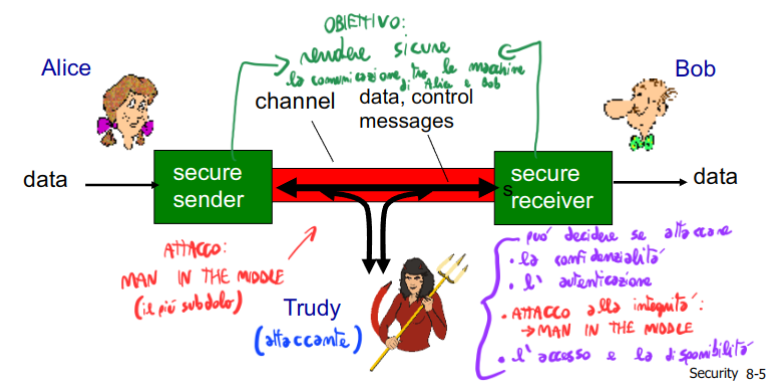
\includegraphics[width=10cm]{img/trudy_bob_alice.png}
\end{center}

Vabbuò passiamo alla sezione sucessiva:
\section{Principi di crittografa}
Partiamo dalla defnizione

\dfn{crittografa}{
    si \textbf{crittografa} la disciplina che studia le tecniche per proteggere le informazioni trasformandole in un formato illeggibile per chi non è autorizzato, consentendo solo ai destinatari legittimi di decifrarle.
}

Nelle reti di comunicazione, i dati trasmessi possono essere intercettati da chiunque abbia accesso al canale di comunicazione, rendendo le informazioni vulnerabili a lettura, modifica o attacchi malevoli. Per proteggere la riservatezza e l’integrità dei dati, si utilizza, quindi, la crittografia, una tecnica che consente di trasformare il testo in chiaro, detto \textit{plaintext}, in un formato incomprensibile chiamato testo cifrato o \textit{ciphertext}, attraverso l’applicazione di un algoritmo di cifratura.

L’obiettivo della crittografia è garantire che, anche se un malintenzionato intercettasse il messaggio durante la trasmissione, non sarebbe in grado di comprenderne il contenuto senza la conoscenza della chiave segreta. Solo il destinatario legittimo, in possesso della chiave corretta, può applicare un algoritmo di decifratura per convertire il testo cifrato nuovamente in testo leggibile.

Va sottolineato che gli algoritmi di cifratura e decifratura sono generalmente pubblici e noti a tutti. Tuttavia, la sicurezza della crittografia si basa sulla segretezza della cosiddetta \textit{chiave crittografica}, ovvero una sequenza di bit utilizzata all'interno di un algoritmo di cifratura per trasformare un messaggio in un formato sicuro e, successivamente, per riconvertirlo nel suo stato originale. Questa chiave viene generata all'inizio della comunicazione tra mittente e destinatario e loro e solo loro ne sono a conoscenza.

Adesso un'introduzione all'algebra della crittografia

Si ha:
\begin{itemize}
    \item $m$: plaintext
    \item $K_A(m)$: ciphertext, encrypted with key $K_A$
    \item $m = K_B(K_A(m))$: plaintext ripristinato grazie alla chiave $K_B$
\end{itemize}

Si noti la seguente immagine (con appunti bonziani):
\begin{center}
    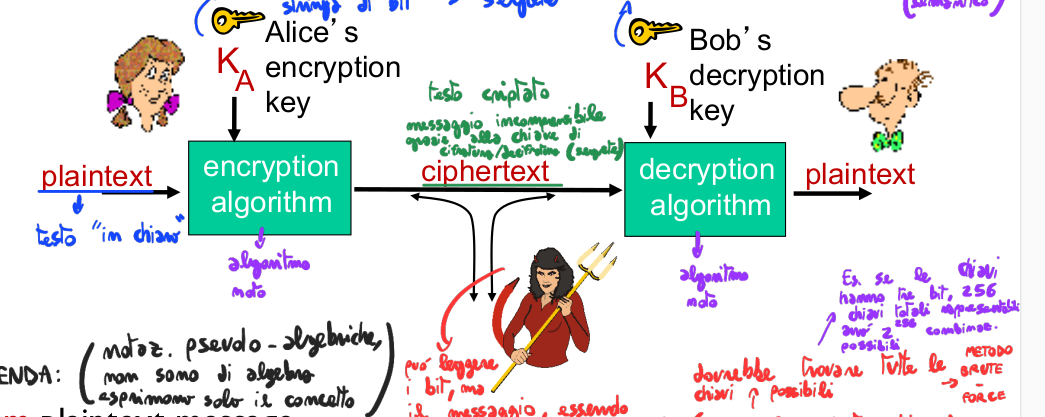
\includegraphics[width=10cm]{img/crittografia.png}
\end{center}

\subsection{Attaccare uno schema di crittografia}

Gli attacchi crittografici mirano a violare la sicurezza di un sistema di cifratura. Ne esistono diversi tipi:
\begin{enumerate}
    \item \textbf{Cipher-text only attack}, l'attaccante possiede solo il testo cifrato a disposizione e per decifrare il messaggio ha due approcci possibile:
    \begin{itemize}
        \item \textbf{Forza bruta}: prova tutte le chiavi possibili
        \item \textbf{Analisi statistica}: cerca pattern ripetuti nei dati cifrati
    \end{itemize}
    \item \textbf{known-plaintext attack}: Trudy possiede sia il testo cifrato che il corrispondente testo in chiaro. Con queste informazioni, cerca di scoprire la chiave di cifratura o il meccanismo utilizzato, così da poter decifrare altri messaggi cifrati dallo stesso sistema.
    
    \ex{}{
    Se Trudy sa che nel testo in chiaro compare la parola "hello" e trova nel messaggio cifrato la sequenza "JGRRG", può iniziare a costruire un dizionario di corrispondenze tra lettere:

    \begin{itemize}
        \item $h \to J$
        \item $e \to G$
        \item $l \to R$
        \item $o \to G$
    \end{itemize}
    }
    
\end{enumerate}

\nt{un buon metodo per evitare questi attacchi è rendere lo spazio delle chiavi il più vasto possibile e utilizzare algoritmi sicuri che resistano alle analisi statistiche}
\subsection{Crittografia a chiave simmetrica}
Adesso entriamo nel vivo della difesa cazzo
\dfn{Crittografia a chiave simmetrica}{
    mittente e destinatario condividono la stessa chiave segreta $K_S$ per cifrare e decifrare i messaggi
}

I pratica il mittente (Alice) cirfra il plaintext con l'algoritmo di cifratura usando la chiave $K_S$ottenendo il ciphertext, Bob riceve il ciphertext e lo decifra usando lo stesso algoritmo e la chiave $K_S$, recuperando il messaggio originale
\begin{center}
    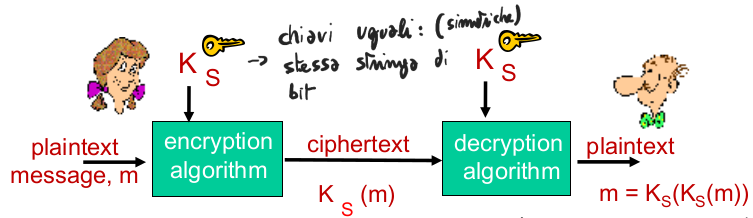
\includegraphics[width=10cm]{img/CHIAVE_SIMMETRICA.png}
\end{center}

Per implementare la chiave simmetrica esistono diverse tecniche

\subsubsection{Cifrario a sostituzione}

\dfn{Cirfrario a sostituizione}{
    Un \textbf{cifrario a sostituzione} è una tecnica di cifratura in cui ogni lettera del testo in chiaro viene sostituita con un'altra lettera secondo un mapping predefinito
}

\paragraph{Cifrario monolitico} Tra i vari tipi di cifrario a sostruzioni vi è il cifrario monolitico dove ogni lettera dell'alfabeto viene sostituita da un'altra lettera fissa

\ex{Cifrario monolitico}{
    \begin{itemize}
        \item Alfabeto in chiaro: abcdefghijklmnopqrstuvwxyz

        \item Alfabeto cifrato: mnbvcxzasdfghjklpoiuytrewq
        \item Messaggio originale: bob. i love you. alice
        \item Messaggio cifrato: nkn. s gktc wky. mgsbc
    \end{itemize}
}

Tuttavia è poco sicuro perché mantiene la frequenza delle lettere originali e lo rende particolarmente vulnerabile alle analisi delle frequenze


\section{Firewall e IDS}

Innanzi definiamo che cos'è un \textit{Firewall}

\dfn{Firewall}{
        Si definisce \textbf{Firewall} un sistema di sicurezza che isola una rete interna di un'organizzazione da internet, controllando e filtrando il traffico di rete in entrata e uscita in base a regole di sicurezza definite dette di \texttt{ACCESS} o \texttt{DENIED}
}

L'idea del Firewall è che l'esterno di una rete è composta dai cosiddetti "cattivi ragazzi" che la mamma non vi raccomanderebbe come compagni d'uscita, mentre l'interno della rete è composta da "bravi ragazzi" di cui fidarsi, lo scopo del sistema è, quindi, separare i buoni dai cattivi

\begin{center}
    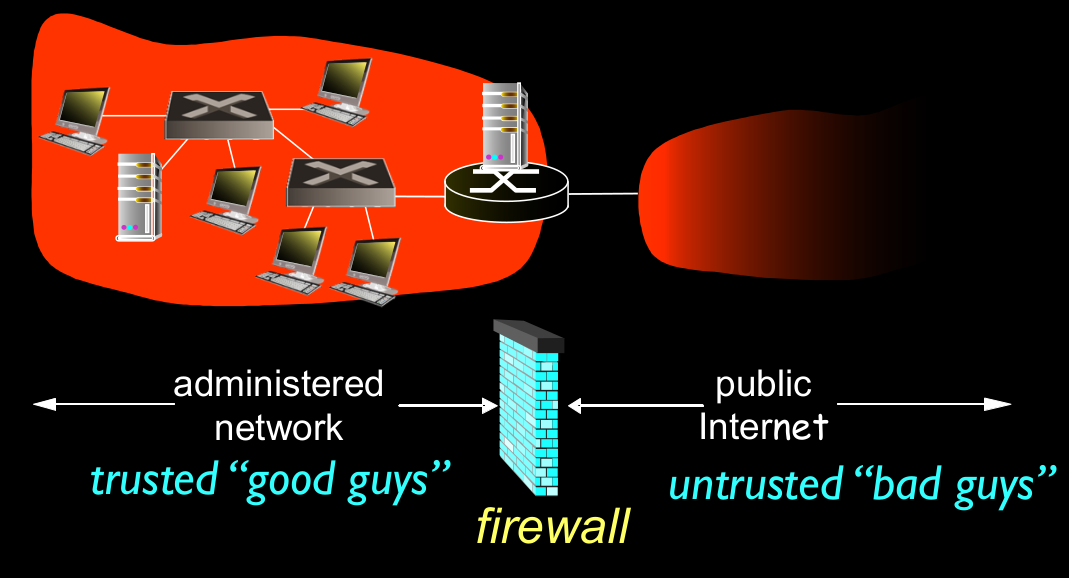
\includegraphics[width=10cm]{img/buoni_cattivi_e_firewall.png}
\end{center}

Il Firewall si rivela utile per principalmente tre motivi:
\begin{itemize}
    \item \textbf{Prevenzione degli attacchi Denial of Service (Dos)}: tipologia di attacco informatico che mira a rendere inaccessibili o indisponibili i servizi di una rete ad utenti legittimi
    
    Un esempio è il \textbf{SYN flooding} in cui un attaccante invia molte richieste di connessione false, esaurendo le risorse del server sovraccaricandolo e impedendo connessioni legittime

    \item \textbf{Protezione dei dati interni da accessi non autorizzati}: ovvero impedisce che gli attaccanti possona \textit{modificare o rubare dati sensibili}
    
    Un esempio classico è un attaccante che sostituisce il sito web di un'organizzazione con un contenuto malevolo.

    \item \textbf{Accesso selettivo e autorizzato alla rete interna}: Permette l’accesso solo a utenti o dispositivi autenticati, migliorando la sicurezza
\end{itemize}

Esistono tre tipi di tipoligie di Firewall che approfonoidremo nel dettaglio:
\begin{itemize}
    \item \textbf{Stateless Packet Filter}: Controlla ogni pacchetto singolarmente, senza tenere traccia delle connessioni
    \item \textbf{Statefull Packet Filter}: Tiene traccia dello stato delle connessioni (es. richieste e risposte)  
    \item \textbf{Application Gateway} (proxy Firewall): controlla il traffico a livello applicativo (es. HTTP, FTP, e.mail), filtrando così le informazioni che all'interno dei protocolli del livello (ad esempio il contenuto di una mail)
\end{itemize}

Si notino nel dettaglio
\subsection{Stateless Packet Filtering}

\dfn{Stateless Packet Filtering}{
    Lo \textbf{Stateless Packet Filtering} è una tecnica di sicurezza di rete in cui un firewall esamina ogni pacchetto individualmente, senza tener conto delle connessioni stabilite in precedenza. Questo significa che ogni pacchetto è valutato isolatamente sulla base di un insieme di regole predefinite
}
Di solito un firewall con filtraggio stateless è implementato su un router che collega una rete interna a internet. Il router analizza ogni pacchetto in ingresso e in uscita e decide se bloccarlo o lasciarlo in base a regole definite nelle cosiddette "\textbf{white list}" (pacchetti che possono passare) e o "\textbf{black list}" (lista di pacchetti da bloccare)

Il firewall prende decisioni basandosi su parametri del pacchetto, tra cui:
\begin{itemize}
    \item \textbf{IP} del mittente e destinatario
    \item \textbf{Numero di porta TCP/UDP} del mittente e destinatario
    \item \textbf{Tipo di messaggio ICMP} bloccando, ad esempio, attacchi di scansione provenienti dall'esterno
    \item \textbf{bit SYN e ACK nei pacchetti TCP}: Il firewall può, ad esempio, bloccare pacchetti con SYN in entrata per impedire connessioni indesiderate dall'esterno
\end{itemize}

Qui degli esempietti:
\ex{Bloccare tutti i pacchetti con protocollo UDP o Telnet}{
    \begin{itemize}
        \item \textbf{Regola}: blocca i pacchetti in entrata e in uscita se il protocollo IP è 17 (UDP) e se con la porta di origine o desitinazione è 23
        \item \textbf{Risultato}: Tutto il traffico UDP  e telnet vengono bloccati
    \end{itemize}
}

\ex{Bloccare pacchetti TCP in ingresso con ACK=0}{
    \begin{itemize}
        \item \textbf{Regola}: blocca tutti i pacchetti TCP in ingresso se il bit ACK = 0
        \item \textbf{Risultato}:Le connessioni in entrata non possono essere iniziate da un host esterno verso la rete interna e le connessioni in uscita funzionano normalmente, perché il traffico di ritorno (che ha ACK=1) è consentito.
    \end{itemize}
}

Riporto qui una tabella con altri esempi:
\begin{center}
    \begin{tabularx}{\textwidth}{|X|X|}
        \hline
        \textbf{Politica} & \textbf{Impostazione Firewall} \\
        \hline
        Nessun accesso Web esterno. & Elimina tutti i pacchetti in uscita verso qualsiasi indirizzo IP, porta 80 \\
        \hline
        Nessuna connessione TCP in entrata, tranne quelle per il server Web pubblico dell'istituzione. & Elimina tutti i pacchetti TCP SYN in entrata verso qualsiasi IP tranne 130.207.244.203, porta 80 \\
        \hline
        Impedisci alle Web-radio di consumare la larghezza di banda disponibile. & Elimina tutti i pacchetti UDP in entrata - tranne DNS e broadcast del router. \\
        \hline
        Impedisci alla tua rete di essere utilizzata per un attacco DoS smurf. & Elimina tutti i pacchetti ICMP diretti a un indirizzo di “broadcast” (ad esempio, 130.207.255.255). \\
        \hline
        Impedisci alla tua rete di essere tracciata & Elimina tutto il traffico ICMP TTL scaduto in uscita \\
        \hline
        \end{tabularx}
\end{center}

\subsubsection{Access control list}
\dfn{Liste di controllo d'accesso}{
    Le \textbf{ACL} sono tabelle di regole applicate, \textit{con priorità dall'alto verso il basso}, ai pacchetti in arrivo per decidere se consentire (allow) o bloccare (deny) il traffico di rete
}

Queste tabelle sono il vero e proprio cuore pulsante del Firewall e indicano quale pacchetto può passare e chi no
\ex{ACL}{
    \begin{center}
        \begin{tabularx}{0.5\textwidth}{|l|l|l|l|l|l|l|}
            \hline
            \textbf{azione} & \textbf{indirizzo sorgente} & \textbf{indirizzo destinazione} & \textbf{protocollo} & \textbf{porta sorgente} & \textbf{porta destinazione} & \textbf{flag bit} \\
            \hline
            allow & 222.22/16 & outside of 222.22/16 & TCP & $>$ 1023 & 80 & any \\
            \hline
            allow & outside of 222.22/16 & 222.22/16 & TCP & 80 & $>$ 1023 & ACK \\
            \hline
            allow & 222.22/16 & outside of 222.22/16 & UDP & $>$ 1023 & 53 & --- \\
            \hline
            allow & outside of 222.22/16 & 222.22/16 & UDP & 53 & $>$ 1023 & --- \\
            \hline
            deny & all & all & all & all & all & all \\
            \hline
        \end{tabularx}
            
    \end{center}
}
\subsubsection{Criticità}
Un serio problema dei Firewall Stateless che potrebbero lasciare passare pacchetti che non hanno senso nel contesto di una connessione.
Esempio:
\begin{itemize}
    \item Un pacchetto con destinazione porta 80 (HTTP) e ACK=1 arriva dall'esterno
    \item Il firewall stateless lo accetta, anche se nessuna connessione HTTP è stata avviata da un client interno.
    \item Un attaccante potrebbe sfruttare questa debolezza per inviare pacchetti falsi alla rete interna
\end{itemize}

Per porre rimedio a questi tipi di problemi si veda la tipoligia di firewall sucessiva

\subsection{Stateful packet filtering}
\dfn{Stateful packet filtering}{
    Lo \textbf{Stateful packet filtering} è una tecnica di filtraggio di pacchetti tenendo traccia delle connessioni attive e delle loro fasi
}
Un firewall stateful tiene traccia di ogni connessione TCP attiva e controlla le tre fasi fondamentali della connessione TCP (assicurandosi che ogni pacchetto in entrata o uscita abbia senso):
\begin{itemize}
    \item \textbf{Setup}: Il firewall rileva il pacchetto SYN iniziale, segnalando l'inizio di una connessione
    \item \textbf{Trasferimento dati}: I pacchetti con ACK vengono accettati solo se appartengono a una connessione già avviata
    \item \textbf{Chiusura}: Quando un pacchetto FIN o un timeout segna la fine di una connessione, il firewall non accetta più pacchetti fino a che non se apre un altro
\end{itemize}



\chapter{Il Livello Rete: Il Piano di Controllo (Control Plane)}
Dopo aver analizzato il \textit{data plane}, ovvero come un router inoltra i pacchetti basandosi su una tabella di forwarding, esploriamo ora il \textit{control plane}. Il suo compito è determinare come vengono costruite e aggiornate queste tabelle. È qui che risiede l'intelligenza della rete, incarnata dagli algoritmi di routing.

\section{Introduzione al Piano di Controllo}
Il piano di controllo ha il compito di calcolare i percorsi che i pacchetti devono seguire. Questo processo, chiamato \textbf{routing}, si contrappone al \textbf{forwarding} (l'azione meccanica di inoltro dei pacchetti). L'obiettivo di un algoritmo di routing è popolare le tabelle di forwarding dei router con percorsi "buoni", ovvero a costo minimo.

Come visto in precedenza, il control plane può essere implementato in due modi:
\begin{itemize}
    \item \textbf{Per-Router Control Plane (Tradizionale)}: Ogni router esegue un algoritmo di routing e comunica con gli altri router per calcolare in modo distribuito la propria tabella di forwarding.
    \item \textbf{Logically Centralized Control Plane (SDN)}: Un controller centrale calcola tutte le tabelle e le distribuisce ai router, che agiscono come semplici esecutori.
\end{itemize}

In questa sezione ci concentreremo sul primo approccio, quello tradizionale, che è alla base dei protocolli storici di Internet.

\section{Algoritmi di Routing}
Per un algoritmo di routing, la rete è un \textbf{grafo}, dove i nodi sono i router e gli archi sono i link fisici tra di essi. A ogni arco è associato un \textbf{costo}, che può rappresentare la distanza, il ritardo, o essere inversamente proporzionale alla banda. L'obiettivo dell'algoritmo è trovare il percorso a costo minimo tra una sorgente e una destinazione.

\subsection{Classificazione degli Algoritmi di Routing}
Gli algoritmi di routing si classificano principalmente secondo due criteri:
\begin{enumerate}
    \item \textbf{Globali vs. Decentralizzati}:
    \begin{itemize}
        \item \textbf{Algoritmi Link-State (Globali)}: Ogni router possiede una conoscenza completa della topologia della rete e dei costi di tutti i link. Con questa mappa globale, ogni router può calcolare il percorso migliore in autonomia.
        \item \textbf{Algoritmi Distance-Vector (Decentralizzati)}: Ogni router conosce solo i propri vicini diretti e i costi per raggiungerli. I percorsi vengono calcolati in modo iterativo, attraverso lo scambio di informazioni solo con i router adiacenti. Nessun router ha una visione completa della rete.
    \end{itemize}
    \item \textbf{Statici vs. Dinamici}:
    \begin{itemize}
        \item \textbf{Routing Statico}: I percorsi vengono configurati manualmente e cambiano raramente. Adatto a reti piccole e stabili.
        \item \textbf{Routing Dinamico}: I percorsi vengono aggiornati automaticamente in risposta a cambiamenti nella topologia o nei costi dei link. È l'approccio utilizzato nella maggior parte delle reti moderne.
    \end{itemize}
\end{enumerate}

\subsection{Algoritmi Link-State (LS)}
L'approccio Link-State si basa su un principio semplice: "informa tutti di tutto".
\begin{enumerate}
    \item Ogni router scopre i propri vicini e il costo dei link per raggiungerli.
    \item Queste informazioni (il suo "link state") vengono impacchettate e diffuse a \textbf{tutti gli altri router} della rete tramite un processo chiamato \textit{flooding}.
    \item Al termine di questo processo, ogni router possiede una mappa completa e identica dell'intera rete.
    \item Su questa mappa, ogni router esegue in locale un algoritmo per trovare il percorso a costo minimo verso tutte le destinazioni. L'algoritmo standard per questo compito è l'\textbf{algoritmo di Dijkstra}.
\end{enumerate}

\paragraph{L'Algoritmo di Dijkstra}
L'algoritmo di Dijkstra calcola, da un nodo sorgente `u`, l'albero dei cammini minimi verso tutti gli altri nodi del grafo. Procede in modo iterativo: a ogni passo, aggiunge all'insieme dei nodi `N'` di cui si conosce il percorso definitivo, il nodo `w` non ancora in `N'` che ha il costo minimo attuale. Successivamente, aggiorna i costi di tutti i vicini di `w`.

\ex{Esempio di Dijkstra}{
    Dato il grafo seguente, calcoliamo i percorsi a costo minimo a partire dal nodo `u`.

    % \begin{center}
    %     \includegraphics[width=9cm]{img/Dijkstra's algorithm example graph}
    % \end{center}

    L'algoritmo procede per passi, aggiornando la tabella dei costi. Alla fine, il risultato per il nodo `u` sarà la seguente tabella di forwarding:

    \begin{center}
        \begin{tabular}{|c|c|}
            \hline
            \textbf{destination} & \textbf{link} \\ \hline
            v & (u,v) \\ \hline
            x & (u,x) \\ \hline
            y & (u,x) \\ \hline
            w & (u,x) \\ \hline
            z & (u,x) \\ \hline
        \end{tabular}
    \end{center}

    Questo significa che per raggiungere `y`, `w` o `z`, `u` deve prima inviare il pacchetto al suo vicino `x`.
}

\subsection{Algoritmi Distance-Vector (DV)}
L'approccio Distance-Vector è decentralizzato e si basa sul principio "informa solo i tuoi vicini". Ogni router conosce molto poco della rete, ma collabora con i vicini per costruire una visione globale.

L'algoritmo si basa sull'equazione di \textbf{Bellman-Ford}:
$$ d_x(y) = \min_{v} \{ c(x,v) + d_v(y) \} $$

In parole: il costo minimo per andare da `x` a `y` è il minimo, calcolato su tutti i vicini `v` di `x`, della somma tra il costo per raggiungere il vicino `v` ($c(x,v)$) e il costo che `v` dichiara di avere per raggiungere `y` ($d_v(y)$).

Il processo è iterativo:
\begin{enumerate}
    \item Ogni router mantiene un proprio \textbf{distance vector}, ovvero una stima del costo per raggiungere ogni destinazione.
    \item Periodicamente, ogni router invia il proprio distance vector ai suoi vicini.
    \item Quando un router riceve un nuovo distance vector da un vicino, ricalcola le proprie stime usando l'equazione di Bellman-Ford.
    \item Se i propri costi cambiano, informa a sua volta i suoi vicini.
\end{enumerate}

Questo processo continua finché le stime non convergono ai valori reali.

\paragraph{Problemi del DV: Count-to-Infinity}
Un grosso svantaggio degli algoritmi DV è il problema del "count-to-infinity". Mentre le "buone notizie" (la scoperta di un percorso migliore con costo inferiore) si propagano velocemente, le "cattive notizie" (un aumento del costo di un link o un guasto) si propagano molto lentamente. In caso di guasto, i router possono entrare in un loop in cui si scambiano informazioni di routing errate, facendo crescere il costo di un percorso verso l'infinito prima di rendersi conto che la destinazione non è più raggiungibile.

\subsection{Confronto tra LS e DV}
\begin{itemize}
    \item \textbf{Complessità dei messaggi}: LS richiede la diffusione di informazioni a tutti i nodi ($O(nE)$ messaggi), mentre DV scambia informazioni solo tra vicini.
    \item \textbf{Velocità di convergenza}: LS è più veloce e robusto. DV può essere lento a convergere e soffre del problema del count-to-infinity.
    \item \textbf{Robustezza}: In LS, un router malfunzionante può inviare informazioni errate sul costo dei propri link, ma ogni altro router calcola la propria tabella in autonomia. In DV, l'errore di un router può propagarsi e influenzare le tabelle di molti altri router nella rete.
\end{itemize}

\section{Routing su Internet: Intra-AS e Inter-AS}
Internet è troppo grande per essere gestita da un unico algoritmo di routing. Per garantire la scalabilità, è organizzata gerarchicamente in \textbf{Sistemi Autonomi (AS)}.

\dfn{Sistema Autonomo (AS)}{
    Un insieme di router e reti sotto un'unica amministrazione tecnica, che presenta una politica di routing comune verso il resto di Internet. Esempi sono la rete di un provider (come TIM), di una grande università o di un'azienda come Google.
}

Questa struttura divide il problema del routing in due:
\begin{enumerate}
    \item \textbf{Routing Intra-AS (Interior Gateway Protocol - IGP)}: L'algoritmo di routing utilizzato \textit{all'interno} di un singolo AS. Tutti i router dell'AS eseguono lo stesso protocollo. L'obiettivo principale qui è l'ottimizzazione delle prestazioni (trovare il percorso migliore).
    \item \textbf{Routing Inter-AS (Exterior Gateway Protocol - EGP)}: L'algoritmo utilizzato per scambiare informazioni di raggiungibilità \textit{tra} AS diversi. L'obiettivo qui non è tanto trovare il percorso più performante, quanto implementare le \textbf{politiche} commerciali e di interconnessione tra i provider.
\end{enumerate}

I router al confine di un AS, che si connettono ad altri AS, sono chiamati \textbf{gateway router}.

\subsection{OSPF: Un Protocollo di Routing Intra-AS}
\textbf{OSPF (Open Shortest Path First)} è uno dei protocolli IGP più diffusi su Internet.
\begin{itemize}
    \item È un protocollo di tipo \textbf{Link-State}.
    \item Ogni router in un AS che usa OSPF ottiene una mappa completa dell'AS.
    \item Su questa mappa, ogni router esegue l'\textbf{algoritmo di Dijkstra} per calcolare i percorsi a costo minimo.
    \item "Open" significa che le sue specifiche sono pubbliche (non è proprietario).
    \item Offre funzionalità avanzate come l'autenticazione dei messaggi di routing per la sicurezza e la possibilità di definire percorsi multipli a parità di costo.
\end{itemize}

Per migliorare ulteriormente la scalabilità all'interno di AS molto grandi, OSPF può essere strutturato gerarchicamente, suddividendo l'AS in \textbf{aree}. I router all'interno di un'area conoscono solo la topologia della propria area, riducendo così il sovraccarico di comunicazione e di calcolo.

% \begin{center}
%     \includegraphics[width=10cm]{img/Hierarchical OSPF diagram}
% \end{center}

\section{Routing Inter-AS: il Protocollo BGP}
Mentre protocolli come OSPF gestiscono in modo efficiente il routing \textit{all'interno} di un singolo Sistema Autonomo (AS), è necessario un protocollo diverso per gestire il routing \textit{tra} AS differenti. Questo compito è affidato al BGP.

\dfn{BGP (Border Gateway Protocol)}{
    È il protocollo di routing Inter-AS (o EGP) standard de facto su Internet. È la "colla" che tiene insieme le migliaia di reti dei provider (ISP), permettendo loro di scambiarsi informazioni su quali destinazioni sono raggiungibili attraverso le rispettive reti.
}

BGP permette a ogni AS di:
\begin{itemize}
    \item \textbf{Ottenere informazioni di raggiungibilità} dai propri AS vicini. Questo avviene tramite una sessione \textbf{eBGP} (external BGP) tra i gateway router di confine.
    \item \textbf{Propagare queste informazioni} a tutti i router interni al proprio AS. Questo avviene tramite sessioni \textbf{iBGP} (internal BGP).
    \item \textbf{Determinare le rotte "migliori"} verso le reti esterne, basandosi non solo sulla performance, ma soprattutto su \textbf{politiche} economiche e di interconnessione.
\end{itemize}

\subsection{Path Vector e Politiche di Routing}
A differenza di OSPF, BGP non si basa sul costo dei link, ma è un protocollo \textbf{Path Vector}.
\begin{itemize}
    \item Quando un AS pubblicizza una rotta verso una destinazione, non comunica un semplice costo, ma l'intero percorso di Sistemi Autonomi da attraversare. Questo percorso è contenuto in un attributo chiamato \textbf{AS-PATH}.
    \item L'attributo AS-PATH è fondamentale per prevenire i loop: un router scarta ogni rotta pubblicizzata in cui compare già il numero del proprio AS.
\end{itemize}

La caratteristica più importante di BGP è che la selezione delle rotte è guidata dalla \textbf{policy}. Un provider può decidere, ad esempio, di non far transitare traffico tra due altri provider attraverso la propria rete (perché non ne trarrebbe alcun guadagno). Questa policy viene implementata semplicemente scegliendo di non ri-pubblicizzare certe rotte ai propri vicini.

\ex{Hot Potato Routing}{
    Una comune politica di routing in BGP è l'hot potato routing. Se un router all'interno di un AS ha più possibili uscite per raggiungere una destinazione esterna, sceglierà l'uscita che ha il costo \textit{interno} (calcolato con OSPF) più basso. In pratica, cerca di "liberarsi" del pacchetto il più velocemente possibile, passandolo a un altro AS, anche se questo potrebbe non corrispondere al percorso globale più breve per il pacchetto stesso.
}

\section{Approfondimento sul Control Plane SDN}
Come anticipato, l'approccio \textbf{Software-Defined Networking (SDN)} rappresenta un cambio di paradigma rispetto al routing tradizionale, separando il "cervello" della rete (il control plane) dal "corpo" (il data plane).

\subsection{L'Architettura di un Controller SDN}
Un controller SDN è un sistema software complesso, un vero e proprio "sistema operativo di rete", che può essere scomposto in tre livelli funzionali:
\begin{enumerate}
    \item \textbf{Livello di Comunicazione (Southbound API)}: È l'interfaccia verso il basso, con cui il controller comunica con i dispositivi di rete (gli switch). Il protocollo più comune per questa interfaccia è \textbf{OpenFlow}. Tramite questa API, il controller può installare/modificare le tabelle di flusso e ricevere notifiche dagli switch (es. un link è caduto).
    \item \textbf{Livello di Gestione dello Stato della Rete}: È il cuore del controller. Mantiene una visione centralizzata e costantemente aggiornata dell'intera rete: la topologia (switch e link), le statistiche di traffico, le informazioni sugli host, ecc.
    \item \textbf{Interfaccia per le Applicazioni (Northbound API)}: È l'interfaccia verso l'alto, con cui le \textbf{applicazioni di controllo di rete} interagiscono con il controller per implementare la logica di rete. Queste applicazioni (per il routing, il bilanciamento del carico, il controllo degli accessi) possono leggere lo stato della rete dal controller e usare l'API per programmare il comportamento desiderato, che il controller tradurrà in regole di flusso per gli switch.
\end{enumerate}

% \begin{center}
%     \includegraphics[width=12cm]{img/SDN controller components}
% \end{center}

\ex{Gestione di un guasto in una rete SDN}{
    \begin{enumerate}
        \item Lo switch S1 rileva che un suo link è caduto.
        \item S1 invia un messaggio OpenFlow `Port Status` al controller.
        \item Il controller aggiorna il suo stato interno della rete per riflettere il guasto.
        \item Un'applicazione di routing, che si era registrata per ricevere notifiche sui cambiamenti di topologia, viene attivata.
        \item L'applicazione di routing ricalcola i nuovi percorsi a costo minimo (es. con Dijkstra) basandosi sulla nuova topologia.
        \item L'applicazione istruisce il controller di installare le nuove tabelle di flusso negli switch interessati dal cambiamento.
        \item Il controller traduce queste istruzioni in messaggi OpenFlow `Modify-State` e li invia agli switch, riprogrammando così il forwarding della rete in tempo reale.
    \end{enumerate}
}

\section{ICMP: il Protocollo di Controllo di Internet}

\dfn{ICMP (Internet Control Message Protocol)}{
    Un protocollo di supporto del livello rete, utilizzato da host e router per comunicare informazioni di controllo e, soprattutto, per segnalare errori. I messaggi ICMP non sono pacchetti ordinari, ma sono incapsulati direttamente all'interno di datagrammi IP.
}

Un messaggio ICMP è definito da un campo `Type` e un campo `Code` che ne specificano il significato. I messaggi più comuni includono:
\begin{itemize}
    \item \textbf{Echo Request/Reply (Type 8/0)}: Usati dal comando \textbf{ping} per verificare la raggiungibilità di un host.
    \item \textbf{Destination Unreachable (Type 3)}: Inviato da un router quando non può inoltrare un pacchetto (es. host irraggiungibile, porta non disponibile).
    \item \textbf{Time Exceeded (Type 11)}: Inviato da un router quando scarta un pacchetto perché il suo campo TTL ha raggiunto zero. È il meccanismo alla base di \textbf{traceroute}.
\end{itemize}

\ex{Funzionamento di Traceroute}{
    Traceroute scopre i router su un percorso inviando una serie di pacchetti (tipicamente UDP) verso la destinazione:
    \begin{enumerate}
        \item Il primo pacchetto viene inviato con un TTL=1. Il primo router lungo il percorso lo scarta e invia indietro un ICMP `Time Exceeded`.
        \item Il secondo pacchetto viene inviato con TTL=2. Il secondo router lo scarta e invia indietro un ICMP.
        \item Il processo continua, aumentando il TTL di uno a ogni passo, fino a quando i pacchetti non raggiungono la destinazione finale.
        \item L'host di destinazione, ricevendo un pacchetto UDP destinato a una porta non in uso, risponde con un ICMP `Destination Port Unreachable`, segnalando la fine del tracciamento.
    \end{enumerate}
}

\section{Reti Wireless e il Livello Fisico}
Le reti wireless hanno rivoluzionato il modo in cui ci connettiamo, ma la loro apparente semplicità nasconde una notevole complessità a livello fisico. La trasmissione di dati attraverso l'etere, senza un mezzo guidato come un cavo, è soggetta a una moltitudine di fenomeni fisici che ne influenzano le prestazioni e l'affidabilità. Questo capitolo esplora i fondamenti delle onde radio, la loro propagazione e i parametri chiave per la progettazione di un sistema wireless.

\section{Fondamenti delle Onde Radio (RF)}

\dfn{Onda a Radiofrequenza (RF)}{
    Un'onda elettromagnetica generata da una corrente alternata ad alta frequenza che scorre in un'antenna. L'antenna agisce come un trasduttore, convertendo la corrente elettrica in onde elettromagnetiche durante la trasmissione e viceversa durante la ricezione.
}

Un'onda elettromagnetica è composta da un campo elettrico e un campo magnetico che oscillano in modo perpendicolare tra loro e alla direzione di propagazione. Questa onda può viaggiare anche nel vuoto, a differenza della corrente elettrica che necessita di un conduttore.

\subsection{Parametri di un'Onda RF}
Un'onda RF sinusoidale è caratterizzata da tre parametri fondamentali, che possono essere modulati per codificare le informazioni (i bit):
\begin{itemize}
    \item \textbf{Ampiezza (Amplitude)}: Rappresenta l'intensità o la potenza del segnale, misurata in Watt (W) o milliwatt (mW). A parità di altre condizioni, un segnale con ampiezza maggiore può percorrere una distanza maggiore prima di diventare troppo debole per essere ricevuto. La potenza necessaria per coprire una certa distanza cresce in modo quadratico (o peggio) con la distanza stessa: per raddoppiare la portata, è necessario quadruplicare la potenza.
    \item \textbf{Frequenza (Frequency)}: Misurata in Hertz (Hz), indica il numero di oscillazioni complete che l'onda compie in un secondo. Le diverse tecnologie wireless operano su bande di frequenza specifiche, assegnate da enti regolatori per evitare interferenze.
    \item \textbf{Lunghezza d'onda (Wavelength, $\lambda$)}: È la distanza fisica tra due picchi consecutivi dell'onda. È inversamente proporzionale alla frequenza, secondo la relazione $\lambda = c/f$, dove $c$ è la velocità della luce. La lunghezza d'onda è un parametro critico per la progettazione delle antenne, la cui dimensione fisica ottimale è tipicamente una frazione ($\frac{1}{2}$ o $\frac{1}{4}$) della lunghezza d'onda del segnale.
\end{itemize}

\ex{Dimensione di un'antenna Wi-Fi}{
    Una rete Wi-Fi opera nella banda a 2.4 GHz ($2.4 \times 10^9$ Hz). La sua lunghezza d'onda è:
    $$ \lambda = \frac{3 \times 10^8 \text{ m/s}}{2.4 \times 10^9 \text{ Hz}} = 0.125 \text{ m} = 12.5 \text{ cm} $$
    Per questo motivo, le antenne dei router Wi-Fi hanno dimensioni dell'ordine di pochi centimetri. Al contrario, una radio FM che trasmette a 100 MHz ha una lunghezza d'onda di 3 metri, richiedendo antenne molto più grandi.
}

\section{Propagazione dei Segnali Wireless}
Nel mondo reale, la propagazione di un'onda RF è tutt'altro che lineare. È influenzata dall'ambiente in modi complessi.

\subsection{Attenuazione e Aree di Copertura}
L'energia di un segnale si disperde man mano che si allontana dalla fonte, un fenomeno noto come \textbf{attenuazione}. Questo definisce tre aree di copertura concentriche attorno a un trasmettitore:
\begin{enumerate}
    \item \textbf{Transmission Range}: L'area in cui il segnale è sufficientemente forte per permettere una comunicazione affidabile e a basso tasso di errore.
    \item \textbf{Detection Range}: L'area in cui il segnale può ancora essere rilevato, ma è troppo debole per estrarre le informazioni in modo corretto.
    \item \textbf{Interference Range}: L'area più esterna, in cui il segnale non è più rilevabile singolarmente ma contribuisce comunque al rumore di fondo, potenzialmente interferendo con altre comunicazioni.
\end{enumerate}

% \begin{center}
%     \includegraphics[width=8cm]{img/Wireless signal propagation ranges}
% \end{center}

\subsection{Effetti Ambientali sulla Propagazione}
Un segnale RF che viaggia attraverso l'ambiente interagisce con gli oggetti che incontra, dando luogo a diversi fenomeni:
\begin{itemize}
    \item \textbf{Shadowing (Assorbimento)}: Ostacoli come muri, edifici o vegetazione assorbono parte dell'energia del segnale, creando "zone d'ombra" con una copertura molto debole. Le frequenze più basse tendono a penetrare gli ostacoli meglio di quelle più alte.
    \item \textbf{Riflessione, Diffrazione e Scattering}: Il segnale viene riflesso da superfici grandi (come un palazzo), diffratto attorno agli spigoli e disperso (scattering) da oggetti piccoli.
\end{itemize}

\subsection{Multipath Propagation e Fase}
A causa di questi fenomeni, il segnale raggiunge il ricevitore attraverso percorsi multipli. Il ricevitore riceve quindi non una singola onda, ma la sovrapposizione del segnale diretto (se presente) e di molteplici "echi" riflessi che arrivano in momenti diversi e con fasi diverse.

\dfn{Multipath Propagation (Propagazione Multipath)}{
    La ricezione di un segnale radio come somma di più repliche dello stesso, che hanno percorso cammini diversi e sono quindi sfasate nel tempo e nella fase.
}

La \textbf{fase} di un'onda descrive la sua posizione nel ciclo di oscillazione. L'effetto del multipath dipende criticamente dalla fase con cui gli echi si sovrappongono:
\begin{itemize}
    \item \textbf{Interferenza Costruttiva}: Se due onde arrivano "in fase", le loro ampiezze si sommano, rafforzando il segnale ricevuto.
    \item \textbf{Interferenza Distruttiva}: Se due onde arrivano "in opposizione di fase" (sfasate di 180°), le loro ampiezze si sottraggono, indebolendo o addirittura annullando completamente il segnale.
\end{itemize}

Questo è il motivo per cui, spostandosi anche solo di pochi centimetri in un ambiente interno, la qualità del segnale Wi-Fi può cambiare drasticamente.

\subsection{Mobilità e Fading}
Quando un dispositivo wireless è in movimento, il suo ambiente multipath cambia continuamente, causando rapide e profonde fluttuazioni della potenza del segnale ricevuto.

\dfn{Fading}{
    La variazione della potenza del segnale ricevuto dovuta agli effetti del multipath. Può essere \textit{short-term} (variazioni veloci dovute all'interferenza) o \textit{long-term} (variazioni lente dovute allo shadowing).
}

\subsection{Polarizzazione}
La polarizzazione descrive l'orientamento del campo elettrico dell'onda radio ed è determinata dall'orientamento fisico dell'antenna. Per un trasferimento di potenza ottimale, l'antenna trasmittente e quella ricevente devono avere la stessa polarizzazione (es. entrambe verticali). Una polarizzazione disallineata (es. una verticale e una orizzontale) introduce una significativa perdita di segnale.

\section{Progettazione e Misura della Potenza nei Sistemi Wireless}
La progettazione di un sistema wireless affidabile richiede un'attenta analisi di tutti i guadagni e le perdite di potenza lungo il percorso, un processo noto come \textit{link budget}.

\subsection{Unità di Misura della Potenza: dB, dBm, dBi}
Poiché la potenza dei segnali RF varia su molti ordini di grandezza, si utilizzano unità logaritmiche per semplificare i calcoli.
\begin{itemize}
    \item \textbf{Decibel (dB)}: È un'unità \textbf{relativa} che esprime il rapporto tra due valori di potenza. Trasforma moltiplicazioni e divisioni in addizioni e sottrazioni.
    \begin{itemize}
        \item $+3 \text{ dB} \approx \times 2$ la potenza
        \item $-3 \text{ dB} \approx / 2$ la potenza
        \item $+10 \text{ dB} = \times 10$ la potenza
        \item $-10 \text{ dB} = / 10$ la potenza
    \end{itemize}
    \item \textbf{dBm}: È un'unità \textbf{assoluta} di potenza. Il valore è espresso in decibel rispetto a un riferimento fisso di 1 milliwatt (mW). Quindi, $0 \text{ dBm} = 1 \text{ mW}$, $20 \text{ dBm} = 100 \text{ mW}$. È l'unità standard per misurare la potenza di trasmettitori e la sensibilità dei ricevitori.
    \item \textbf{dBi}: È un'unità che misura il \textbf{guadagno passivo} di un'antenna. Le antenne reali non irradiano energia uniformemente in tutte le direzioni come una teorica \textbf{antenna isotropica}, ma la concentrano in una direzione preferenziale. Il guadagno in dBi indica di quanti decibel il segnale in quella direzione è più forte rispetto a quello che avrebbe prodotto un'antenna isotropica.
\end{itemize}

\subsection{Potenza Irradiata e Normative}
Le agenzie governative impongono limiti sulla massima potenza che un dispositivo può irradiare per evitare interferenze.

\dfn{EIRP (Equivalent Isotropically Radiated Power)}{
    La potenza totale effettivamente irradiata da un'antenna nella sua direzione di massimo guadagno. Si calcola sommando la potenza in uscita dal trasmettitore (in dBm) e il guadagno dell'antenna (in dBi).
}

Un progettista deve quindi regolare la potenza del trasmettitore in modo che, una volta aggiunto il guadagno dell'antenna, l'EIRP totale non superi i limiti di legge.

\subsection{Il Calcolo del Link Budget}
Il link budget è un bilancio energetico che verifica se una connessione wireless è fattibile.

\dfn{Link Budget}{
    Un calcolo che somma tutti i guadagni (potenza del trasmettitore, guadagno delle antenne) e sottrae tutte le perdite (perdite dei cavi, attenuazione nello spazio libero, ostacoli) per determinare la potenza del segnale che arriva al ricevitore.
}

Questo valore deve essere confrontato con la \textbf{Sensibilità del Ricevitore (Receiver Sensitivity, RS)}, che è la minima potenza (in dBm) necessaria al ricevitore per decodificare correttamente il segnale a una data velocità. Un buon progetto richiede che la potenza ricevuta sia significativamente superiore alla sensibilità, lasciando un \textbf{Fade Margin} (es. 10-20 dB) per far fronte a imprevisti come il fading o le cattive condizioni atmosferiche.
\subsection{Dettagli sulle Unità di Misura della Potenza}
Per progettare e analizzare un sistema wireless, è fondamentale padroneggiare le unità di misura logaritmiche, che semplificano notevolmente i calcoli di guadagni e perdite.

\paragraph{Il Decibel (dB)}
Il Decibel è un'unità \textbf{relativa} utilizzata per esprimere il rapporto tra due livelli di potenza, $P_1$ e $P_2$. La sua definizione è:
$$ \text{dB} = 10 \cdot \log_{10}\left(\frac{P_1}{P_2}\right) $$

Il suo grande vantaggio è che trasforma le moltiplicazioni e divisioni in addizioni e sottrazioni, rendendo i calcoli più intuitivi. Si usano spesso le seguenti regole pratiche:
\begin{itemize}
    \item \textbf{+3 dB}: Raddoppia la potenza (x2).
    \item \textbf{-3 dB}: Dimezza la potenza (/2).
    \item \textbf{+10 dB}: Moltiplica la potenza per 10 (x10).
    \item \textbf{-10 dB}: Divide la potenza per 10 (/10).
\end{itemize}

\ex{Calcolo con i dB}{
    Se un segnale di 100 mW subisce una perdita di 7 dB, la potenza finale è:
    $$-7 \text{ dB} = -10 \text{ dB} + 3 \text{ dB}$$
    Quindi la potenza finale sarà: $(100 \text{ mW} / 10) \times 2 = 20 \text{ mW}$. L'uso dei dB ha trasformato un calcolo complesso in semplici somme.
}

\paragraph{Il dBm e il dBi}
Poiché il dB è relativo, sono state introdotte unità assolute con un punto di riferimento fisso.
\begin{itemize}
    \item \textbf{dBm}: È un'unità di potenza \textbf{assoluta}, dove il riferimento è 1 milliwatt (mW). Pertanto, per definizione:
    $$ 0 \text{ dBm} = 1 \text{ mW} $$
    È l'unità standard per indicare la potenza di un trasmettitore o la sensibilità di un ricevitore. Ad esempio, $20 \text{ dBm} = 100 \text{ mW}$.
    \item \textbf{dBi}: È un'unità che misura il \textbf{guadagno} di un'antenna. Indica di quanti decibel la potenza irradiata dall'antenna in una specifica direzione è maggiore rispetto a quella che sarebbe irradiata da un'antenna isotropica teorica.
\end{itemize}

\section{Le Antenne Wireless}

\dfn{Antenna}{
    Un dispositivo passivo che funge da trasduttore: converte l'energia elettrica guidata da un cavo in onde elettromagnetiche che si propagano nello spazio (in trasmissione) e viceversa (in ricezione).
}

La forma e la dimensione di un'antenna determinano il suo \textbf{diagramma di radiazione} (\textit{radiation pattern}), ovvero come l'energia viene distribuita nello spazio.

\subsection{Tipi di Antenne}
\begin{itemize}
    \item \textbf{Antenna Isotropica}: Un'antenna teorica e ideale che irradia potenza in modo perfettamente uniforme in tutte le direzioni, formando una sfera. È il punto di riferimento (0 dBi) per misurare il guadagno di tutte le antenne reali.
    \item \textbf{Antenne Omnidirezionali}: Irradiano potenza uniformemente sul piano orizzontale, creando un diagramma di radiazione a forma di "ciambella" (toroide). Sono ideali per coprire un'area a 360° attorno a un punto centrale. L'esempio più comune è l'\textbf{antenna a dipolo} dei router Wi-Fi domestici. Un dipolo ad alto guadagno produce una ciambella più piatta e larga, coprendo una maggiore distanza orizzontale a scapito della copertura verticale.
    \item \textbf{Antenne Direzionali}: Concentrano la maggior parte dell'energia in una direzione specifica, formando un "lobo" di radiazione principale. Questo permette di coprire distanze maggiori con meno potenza o di creare collegamenti punto-punto sicuri. Il grado di direzionalità è misurato dal \textbf{beamwidth}, l'ampiezza angolare del lobo principale. Esempi includono le antenne \textbf{Yagi}, \textbf{Patch/Panel} e le \textbf{paraboliche}.
\end{itemize}

% \begin{center}
%     \includegraphics[width=12cm]{img/Diagrams of different antenna radiation patterns}
% \end{center}

\subsection{Utilizzo delle Antenne Direzionali}
Le antenne direzionali sono cruciali per i collegamenti wireless a lunga distanza. Il loro uso richiede però la comprensione di due concetti chiave:
\begin{itemize}
    \item \textbf{Line of Sight (LOS)}: Deve esistere una linea di vista ottica libera da ostacoli tra l'antenna trasmittente e quella ricevente.
    \item \textbf{Zona di Fresnel (Fresnel Zone)}: L'energia RF non viaggia come un raggio laser, ma occupa un volume a forma di ellissoide attorno alla linea di vista. Questa zona deve essere per la maggior parte libera da ostacoli (alberi, edifici). Un'ostruzione significativa della zona di Fresnel può interrompere il collegamento anche se la linea di vista ottica è libera. La dimensione della zona di Fresnel dipende dalla frequenza e dalla distanza del link.
\end{itemize}

\subsection{Concetti Avanzati sulle Antenne}
\begin{itemize}
    \item \textbf{Antenne Settorizzate}: Tipiche delle torri per la telefonia mobile, sono composte da un array di più antenne direzionali, ognuna delle quali copre un "settore" (es. 120°). Questo permette di riutilizzare le stesse frequenze in settori non adiacenti, aumentando la capacità totale della cella.
    \item \textbf{Antenna Diversity}: Una tecnica fondamentale per combattere il fading causato dal multipath. Si utilizzano due o più antenne distanziate di una piccola frazione di lunghezza d'onda. La probabilità che tutte le antenne si trovino contemporaneamente in un punto di interferenza distruttiva è molto bassa. Il ricevitore può quindi scegliere dinamicamente il segnale proveniente dall'antenna con la qualità migliore in un dato istante. È il motivo per cui i moderni router Wi-Fi hanno più antenne.
\end{itemize}

\section{Calcolo del Link Budget: Esempio Pratico}
Il \textbf{link budget} è il calcolo fondamentale nella progettazione di un collegamento wireless, specialmente outdoor. Esso fa un bilancio di tutti i guadagni e le perdite per assicurarsi che il segnale arrivi a destinazione con una potenza sufficiente.

\dfn{Link Budget}{
    La differenza, misurata in dB, tra la potenza del segnale ricevuto e la sensibilità minima del ricevitore. Un link budget positivo indica che il collegamento è fattibile.
}

La formula generale è:
$$ \text{Potenza Ricevuta (dBm)} = P_{TX} + G_{TX} - L_{TX} - L_{FS} - L_{M} + G_{RX} - L_{RX} $$
dove:
\begin{itemize}
    \item $P_{TX}$: Potenza del trasmettitore (dBm)
    \item $G_{TX}, G_{RX}$: Guadagno delle antenne trasmittente e ricevente (dBi)
    \item $L_{TX}, L_{RX}$: Perdite nei cavi e connettori (dB)
    \item $L_{FS}$: Perdita di propagazione nello spazio libero (\textit{Free Space Path Loss}), che dipende da distanza e frequenza (dB).
    \item $L_{M}$: Margine per perdite varie (es. pioggia, fogliame) (dB)
\end{itemize}

Il risultato, `Potenza Ricevuta`, deve essere maggiore della `Sensibilità del Ricevitore` di un valore detto \textbf{Fade Margin}, che garantisce la stabilità del link.

\ex{Calcolo di un Link Budget}{
    Consideriamo un link di 10 km a 2.4 GHz.
    \begin{itemize}
        \item Potenza del Trasmettitore: +15 dBm
        \item Guadagno Antenna TX: +24 dBi
        \item Perdite cavi/connettori TX: -5.4 dB
        \item Path Loss per 10 km a 2.4 GHz: -120 dB
        \item Guadagno Antenna RX: +24 dBi
        \item Perdite cavi/connettori RX: -5.4 dB
        \item \textbf{Guadagno Totale}: $15 + 24 + 24 = +63 \text{ dB}$
        \item \textbf{Perdita Totale}: $-5.4 - 120 - 5.4 = -130.8 \text{ dB}$
        \item \textbf{Potenza Ricevuta}: $+63 - 130.8 = -67.8 \text{ dBm}$
    \end{itemize}
    Se la sensibilità del ricevitore per la velocità desiderata è di -82 dBm:
    $$ \text{Link Budget} = -67.8 \text{ dBm} - (-82 \text{ dBm}) = +14.2 \text{ dB} $$
    Il budget è positivo di 14.2 dB. Se questo valore è considerato un Fade Margin sufficiente, il collegamento è affidabile e non necessita di amplificatori o antenne a più alto guadagno.
}

\chapter{Il Controllo di Accesso al Mezzo (MAC) nelle Reti Wireless}
Nei capitoli precedenti abbiamo esplorato i fondamenti fisici della trasmissione wireless. Ora ci addentriamo nel livello immediatamente superiore, il \textbf{MAC (Medium Access Control)}, per capire come i dispositivi wireless coordinano l'accesso al canale di comunicazione condiviso, un problema molto più complesso rispetto al mondo cablato.

\section{La Sfida del MAC Wireless}
In una rete wireless, tutti i dispositivi comunicano sullo stesso canale broadcast. Se più dispositivi trasmettono contemporaneamente, i loro segnali si sovrappongono e si distruggono a vicenda, generando una \textbf{collisione}. Il compito del protocollo MAC è orchestrare le trasmissioni per minimizzare le collisioni e utilizzare in modo efficiente le scarse risorse a disposizione: la capacità del canale e l'energia delle batterie.

\subsection{L'Inadeguatezza di Ethernet nel Wireless}
Il protocollo MAC per eccellenza delle reti cablate, Ethernet, si basa su un meccanismo chiamato \textbf{CSMA/CD (Carrier Sense Multiple Access with Collision Detection)}.
\begin{itemize}
    \item \textbf{Carrier Sense}: Un dispositivo "ascolta" il canale e trasmette solo se lo percepisce come libero.
    \item \textbf{Collision Detection}: Un dispositivo, mentre trasmette, continua ad ascoltare. Se rileva una collisione, interrompe immediatamente la trasmissione, attende per un tempo casuale e riprova.
\end{itemize}

Questo approccio \textbf{non è praticabile} in un ambiente wireless per due ragioni fondamentali:
\begin{enumerate}
    \item \textbf{Impossibilità della Collision Detection}: Un'antenna radio non può trasmettere e ricevere contemporaneamente sulla stessa frequenza. La potenza del segnale trasmesso è immensamente superiore a quella di qualsiasi segnale in ricezione, rendendo impossibile per il trasmettitore "accorgersi" di una collisione mentre sta avvenendo. La collisione si manifesta solo presso il \textbf{ricevitore}.
    \item \textbf{Problemi del Carrier Sensing (Terminali Nascosti/Esposti)}: Il concetto di canale "libero" o "occupato" è relativo alla posizione. Un dispositivo potrebbe non sentire una trasmissione in corso perché troppo distante dal trasmettitore (problema del \textbf{terminale nascosto}), e iniziare a sua volta una trasmissione che causerà una collisione presso un ricevitore comune.
\end{enumerate}

Di conseguenza, il MAC wireless deve abbandonare la \textit{rilevazione} delle collisioni in favore della loro \textit{prevenzione} (\textbf{Collision Avoidance}).

\section{Classificazione dei Protocolli MAC Wireless}
I protocolli MAC si possono classificare in base a come gestiscono la contesa (\textit{contention}) per il canale.

% \begin{center}
%     \includegraphics[width=13cm]{img/Classification of MAC protocols}
% \end{center}

La distinzione principale è tra:
\begin{itemize}
    \item \textbf{Contention-Free}: L'accesso al canale è regolato in modo da eliminare a priori le collisioni. Questo si ottiene tipicamente tramite un \textbf{coordinatore centralizzato} che assegna a ogni dispositivo il proprio turno per trasmettere (es. tramite \textit{polling} o assegnando slot di tempo fissi - \textit{TDMA}). Garantisce prestazioni prevedibili ma può essere inefficiente.
    \item \textbf{Contention-Based}: Non c'è un coordinatore centrale (o il suo ruolo è limitato). I dispositivi competono per l'accesso al canale, e il protocollo si occupa di risolvere le collisioni quando avvengono. Sono protocolli più flessibili e adatti a traffico "a raffica" (\textit{bursty}). Questi si dividono a loro volta in \textbf{deterministici} e \textbf{probabilistici} (o ad accesso casuale).
\end{itemize}

\subsection{Protocolli ad Accesso Casuale (Random Access)}
Questi protocolli sono il fondamento dei sistemi Wi-Fi moderni e si sono evoluti nel tempo per migliorare l'efficienza.

\paragraph{ALOHA}
È il protocollo più semplice: quando un nodo ha un pacchetto da inviare, lo trasmette immediatamente. Se il pacchetto collide con un altro, il mittente non riceve la conferma (ACK) dal destinatario, attende un tempo casuale e ritrasmette.
\begin{itemize}
    \item \textbf{Vulnerabilità}: Una trasmissione è vulnerabile per un tempo pari al doppio della durata del frame, perché una collisione si verifica se un altro nodo inizia a trasmettere in qualsiasi momento durante questo intervallo.
    \item \textbf{Efficienza}: Molto bassa, con un throughput massimo teorico di circa il 18\%.
\end{itemize}

\paragraph{Slotted ALOHA}
Un miglioramento di ALOHA in cui il tempo è suddiviso in slot discreti di durata pari a un frame. Le stazioni possono iniziare a trasmettere solo all'inizio di uno slot.
\begin{itemize}
    \item \textbf{Vulnerabilità}: La finestra di vulnerabilità si dimezza, poiché le collisioni possono avvenire solo se due stazioni scelgono lo stesso slot.
    \item \textbf{Efficienza}: Il throughput massimo raddoppia, raggiungendo circa il 37\%.
\end{itemize}

\paragraph{CSMA (Carrier Sense Multiple Access)}
Aggiunge il principio "ascolta prima di parlare". Una stazione trasmette solo se sente il canale libero. Questo riduce drasticamente il numero di collisioni, ma non le elimina a causa del ritardo di propagazione.
\begin{itemize}
    \item \textbf{Vulnerabilità}: La finestra di vulnerabilità è legata al tempo di propagazione del segnale.
    \item \textbf{Efficienza}: Molto più alta di ALOHA a bassi carichi, ma le prestazioni crollano a carichi elevati, quando il canale è quasi sempre occupato e le collisioni tra stazioni in attesa diventano frequenti.
\end{itemize}

% \begin{center}
%     \includegraphics[width=10cm]{img/Throughput comparison of random access protocols}
% \end{center}

\section{La Dimensione Spaziale: Terminali Nascosti ed Esposti}
Gli algoritmi visti finora si concentrano sul dominio del tempo, ma nel wireless è fondamentale gestire anche il dominio dello spazio.

\dfn{Problema del Terminale Nascosto (Hidden Terminal)}{
    Si verifica quando un nodo A è visibile a un ricevitore C, ma non a un altro nodo B, che è anch'esso visibile a C. Se A sta trasmettendo a C, B non lo sente, percepisce il canale come libero e potrebbe iniziare una sua trasmissione verso C, causando una collisione che corrompe entrambi i messaggi.
}

% \begin{center}
%     \includegraphics[width=9cm]{img/Hidden terminal problem diagram}
% \end{center}

\dfn{Problema del Terminale Esposto (Exposed Terminal)}{
    È la situazione opposta. Il nodo B sta trasmettendo al nodo A. Il nodo C, vicino a B ma lontano da A, vorrebbe trasmettere a D. C sente la trasmissione di B, percepisce il canale come occupato e si astiene dal trasmettere, anche se la sua trasmissione non avrebbe interferito con la ricezione di A. È uno spreco di capacità del canale.
}

\subsection{La Soluzione: l'Handshake RTS/CTS}
Per risolvere in particolare il problema del terminale nascosto, sono stati introdotti meccanismi di \textbf{Collision Avoidance} basati su un handshake a quattro vie.

\dfn{Handshake RTS/CTS (Request to Send / Clear to Send)}{
    Un meccanismo in cui un trasmettitore, prima di inviare un lungo pacchetto di dati, "prenota" il canale inviando un breve pacchetto di controllo \textbf{RTS} (Richiesta di Invio). Il ricevitore, se è pronto, risponde con un pacchetto \textbf{CTS} (Pronto a Ricevere).
}

Questo semplice scambio risolve il problema:
\begin{itemize}
    \item Il pacchetto CTS viene sentito da tutti i nodi vicini al \textbf{ricevitore} (incluso il terminale nascosto B).
    \item Il messaggio CTS contiene la durata della trasmissione che sta per avvenire.
    \item Qualsiasi nodo che sente il CTS sa che deve rimanere in silenzio per quella durata, anche se non sente l'RTS o il trasmettitore stesso.
\end{itemize}

In questo modo, lo spazio attorno al ricevitore viene "silenziato" per la durata della trasmissione, evitando collisioni da parte di terminali nascosti. L'uso di RTS/CTS introduce un overhead, e per questo motivo viene tipicamente attivato solo per pacchetti di dati che superano una certa soglia di dimensione.
\subsection{Limiti di RTS/CTS e Variazioni sul Tema}
L'handshake RTS/CTS, sebbene efficace contro il problema del terminale nascosto, non è una panacea e introduce le sue complessità.

\paragraph{Vulnerabilità e Overhead}
L'uso di RTS/CTS aggiunge un sovraccarico significativo: prima di ogni pacchetto di dati, è necessario scambiare due pacchetti di controllo, consumando tempo e capacità del canale. Per questo motivo, il suo utilizzo è tipicamente limitato ai pacchetti di grandi dimensioni. Inoltre, non è immune da attacchi: un malintenzionato potrebbe inondare la rete di pacchetti CTS falsi (\textit{CTS flooding}), silenziando di fatto tutti i nodi nell'area e causando un attacco Denial of Service.

\paragraph{Evoluzioni del Protocollo: MACA, MACAW, FAMA}
L'idea di base del Collision Avoidance si è evoluta attraverso una serie di protocolli di ricerca:
\begin{itemize}
    \item \textbf{MACA (Multiple Access with Collision Avoidance)}: Formalizza l'uso di RTS/CTS, eliminando del tutto il carrier sensing e affidandosi unicamente all'handshake per gestire la contesa, che di fatto avviene attorno al ricevitore.
    \item \textbf{MACAW}: Migliora MACA introducendo un pacchetto \textbf{ACK} dopo la ricezione dei dati. Questo crea un handshake a 4 vie (\textbf{RTS-CTS-DATA-ACK}) che non solo previene le collisioni, ma fornisce anche un meccanismo di riscontro per la trasmissione affidabile a livello MAC.
    \item \textbf{FAMA}: Reintroduce il \textbf{carrier sensing} prima dell'invio dell'RTS. Combina così i vantaggi di entrambi gli approcci: si "ascolta" il canale per evitare collisioni ovvie e si usa l'handshake per risolvere i problemi spaziali più complessi come i terminali nascosti.
\end{itemize}

\section{Il MAC dello Standard IEEE 802.11 (Wi-Fi)}
Lo standard IEEE 802.11, su cui si basano tutte le reti Wi-Fi, definisce un'architettura MAC ibrida e sofisticata, progettata per operare in due modalità diverse.

\subsection{Le Due Funzioni di Coordinamento: DCF e PCF}
Il MAC 802.11 è composto da due meccanismi che possono coesistere, alternandosi nel tempo all'interno di una \textbf{super-frame}:
\begin{enumerate}
    \item \textbf{DCF (Distributed Coordination Function)}: È la modalità fondamentale, obbligatoria e più comune. È un meccanismo \textbf{distribuito e basato sulla contesa} (\textit{contention-based}). Utilizza l'algoritmo \textbf{CSMA/CA} (Carrier Sense Multiple Access with Collision Avoidance) per gestire l'accesso. Offre un servizio \textit{best-effort} senza garanzie sulla qualità del servizio (QoS). È la modalità usata nelle reti domestiche e nelle configurazioni \textit{ad-hoc}.
    \item \textbf{PCF (Point Coordination Function)}: È una modalità opzionale e \textbf{centralizzata, priva di contesa} (\textit{contention-free}). Richiede un coordinatore centrale, l'\textbf{Access Point (AP)}, che gestisce l'accesso al canale tramite \textit{polling}: interroga a turno le stazioni, dando loro il permesso di trasmettere. Questo elimina le collisioni e permette di offrire garanzie di base sulla banda e sul ritardo (soft QoS).
\end{enumerate}

\subsection{Gli Interframe Spaces (IFS): la Base della Priorità}
Per orchestrare l'alternanza tra DCF, PCF e le risposte immediate (come gli ACK), lo standard 802.11 definisce degli intervalli di tempo di attesa obbligatori, chiamati \textbf{Interframe Spaces}, di diversa durata. La regola è semplice: chi deve attendere per meno tempo ha una priorità più alta.
\begin{itemize}
    \item \textbf{SIFS (Short IFS)}: L'intervallo più breve. Ha la priorità più alta ed è usato per operazioni che devono avvenire immediatamente dopo una trasmissione, come l'invio di un CTS in risposta a un RTS, o di un ACK in risposta a un pacchetto di dati.
    \item \textbf{PIFS (PCF IFS)}: Intervallo di media durata. Viene usato dall'Access Point. Se il canale è libero per un tempo pari a un PIFS, l'AP ha il diritto di prenderne il controllo per avviare una fase PCF (contention-free).
    \item \textbf{DIFS (DCF IFS)}: L'intervallo più lungo. Una stazione che deve inviare un nuovo pacchetto di dati in modalità DCF deve attendere che il canale sia libero per almeno un tempo pari a un DIFS.
\end{itemize}

Questa gerarchia ($SIFS < PIFS < DIFS$) garantisce che un ACK abbia sempre la precedenza su un poll del PCF, che a sua volta ha la precedenza su una nuova trasmissione dati in DCF.

% \begin{center}
%     \includegraphics[width=12cm]{img/IEEE 802.11 Interframe Spaces (IFS)}
% \end{center}

\subsection{La Distributed Coordination Function (DCF) in Dettaglio}
La DCF è il cuore del Wi-Fi e si basa sul CSMA/CA con un meccanismo di backoff per evitare le collisioni.

\paragraph{La Procedura di Backoff}
Quando una stazione vuole trasmettere e rileva che il canale è libero da almeno un DIFS, non trasmette immediatamente. Per evitare che più stazioni in attesa trasmettano contemporaneamente, avvia una procedura di attesa casuale:
\begin{enumerate}
    \item \textbf{Scelta del contatore}: La stazione sceglie un numero intero casuale, il \textit{backoff counter}, in un intervallo $[0, CW]$, dove $CW$ è la \textbf{Contention Window} (finestra di contesa).
    \item \textbf{Conto alla rovescia}: La stazione continua a monitorare il canale. Per ogni \textit{slot time} in cui il canale rimane libero, decrementa il suo contatore. Se il canale diventa occupato, il contatore viene "congelato" e riprenderà il conto alla rovescia non appena il canale sarà di nuovo libero per un DIFS.
    \item \textbf{Trasmissione}: La stazione trasmette il suo frame solo quando il suo contatore di backoff ha raggiunto lo zero.
\end{enumerate}

\paragraph{Binary Exponential Backoff (BEB)}
Per adattarsi al livello di congestione della rete, la dimensione della Contention Window non è fissa.
\begin{itemize}
    \item All'inizio (o dopo una trasmissione riuscita), la $CW$ è impostata al suo valore minimo ($CW_{min}$).
    \item A ogni collisione (rilevata dalla mancata ricezione di un ACK), la stazione \textbf{raddoppia} la dimensione della $CW$, fino a un valore massimo ($CW_{max}$).
\end{itemize}

Questo meccanismo, noto come \textbf{Binary Exponential Backoff}, aumenta esponenzialmente l'intervallo da cui viene estratto il contatore casuale, "sparpagliando" maggiormente nel tempo i tentativi di ritrasmissione e riducendo la probabilità di ulteriori collisioni.


\end{document}

